\documentclass[openany,twoside,svgnames,x11names]{book}

%%%% paquetes de geom
\usepackage{calc}
\usepackage{pifont}
\usepackage{tikz}
\usepackage{fancyhdr}
\usetikzlibrary{shapes,snakes,positioning}
%\usepackage{bodegraph}
%\usetikzlibrary{intersections}
%\usetikzlibrary{calc}
%\usetikzlibrary{positioning}
%\usetikzlibrary{backgrounds,fit}
%\pgfdeclarelayer{myback}
%\pgfsetlayers{myback,main}
\pgfdeclarelayer{background}
\pgfdeclarelayer{foreground}
\pgfsetlayers{background,main,foreground}
\usepackage{wallpaper}
\usepackage{pgf}
\usetikzlibrary{calc}
\usetikzlibrary{arrows}
\usepackage{epstopdf}
\usepackage{floatflt}
\usepackage{pgfplots}
\usepackage{setspace}
\usepackage{amsmath,amssymb}
%\usepackage{booktabs}
\usepackage{courier}
\usepackage{units}
\usepackage{url}
\usepackage{float}
\usepackage{mathpazo}
\usepackage{amsfonts}
\usepackage{fancyvrb}
\usepackage{multicol}
\usepackage{multirow}
\usepackage[utf8x]{inputenc}
\usepackage[calcwidth]{titlesec}
\usepackage{titletoc}
\usepackage{enumerate}
\usepackage{comment}
\usepackage{ifthen}
\usepackage{cancel}
\usepackage{layout}
\usepackage{footnote}
\usepackage{etex}%si pgfplot tiene problemas con new dim
%%%%%%%%%%%%%%%%%%%%%
%\usepackage{minitoc}
%\setcounter{minitocdepth}{2}
%\setlength{\mtcindent}{24pt}
%\renewcommand{\mtcfont}{\tiny\rm}
%\renewcommand{\mtcSfont}{\tiny\bf}
%\setlength\textwidth{16.6cm}
%\setlength\textheight{22.9cm}
%\topmargin -1.0cm
%\setlength\oddsidemargin{(\paperwidth-\textwidth)/2 - 1in}
%\setlength\topmargin{(\paperheight-\textheight
%-\headheight-\headsep-\footskip)/2 - 1in}
\usepackage[paperheight=27.9cm,%
paperwidth=21.6cm,%
%centering,%
%textheight=22.9cm,
left=2cm,%
right=3cm,%
top=2cm,%
bottom=2cm,%
headheight=0.5cm,%
headsep=20pt,%
footskip=1cm,%
marginparsep=20pt,
pdftex=false,
letterpaper
]{geometry}
%\setlength\textwidth{16.6cm}
%\setlength\textheight{22.9cm}
%\setlength\oddsidemargin{(\paperwidth-\textwidth)/2 - 1in}
%\setlength\topmargin{(\paperheight-\textheight
%-\headheight-\headsep-\footskip)/2 - 1in}
%\usepackage[paperheight=27.9cm,%
%paperwidth=21.6cm,%
%%centering,%
%left=1.5cm,%
%right=1.5cm,%
%margin=2.5cm,
%top=2.3cm,%
%bottom=2.3cm,%
%headheight=0.5cm,%
%headsep=10pt,%
%footskip=1cm,%
%marginparsep=20pt,
%pdftex=false
%%letterpaper
%]{geometry}
\usepackage[frame,letter,cam]{crop}
\usepackage{microtype,soul,filecontents}
\usepackage{pgf}
\usepackage{bbding}
\usepackage{lettrine,caption,multicol}
\usepackage{xcolor}
\usepackage{lipsum,soul}
\usepackage{palatino}
\usepackage{calligra}
\usepackage[T1]{fontenc}
\usepackage[listings,theorems]{tcolorbox}
%\usepackage[charter]{mathdesign}
% \def\rmdefault{bch} % not scaled
% \def\ttdefault{blg}
\usepackage{xcolor,filecontents,ragged2e}
\usepackage{floatflt}
\makeatletter

%%%%%%%%Colores que usaremos

\definecolor{theblue}{rgb}{0.02,0.04,0.48}
\definecolor{thered}{rgb}{0.65,0.04,0.07}
\definecolor{thegreen}{rgb}{0.06,0.44,0.08}
\definecolor{thegrey}{gray}{0.5}
\definecolor{theshade}{gray}{0.94}
\definecolor{theframe}{gray}{0.75}
\definecolor{burl}{rgb}{0.27,0.22,0.20}
\definecolor{caper}{rgb}{0.36,0.46,0.23}
\definecolor{rhodo}{rgb}{0.58,0.63,0.45}
\definecolor{wood}{rgb}{0.61,0.51,0.43}
\definecolor{mesh}{rgb}{0.97,0.93,0.81}

\lstloadlanguages{[LaTeX]TeX, [primitive]TeX}

% Emphasis
\newcommand\emphasis[2][thered]{\lstset{emph={newcommand,def,gdef,#2},
   emphstyle={\ttfamily\textcolor{#1}}}}%

\lstset{language={[LaTeX]TeX},
      escapeinside={{(*@}{@*)}}, 
       numbers=left, gobble=0,
       stepnumber=1,numbersep=5pt, 
       numberstyle={\footnotesize\color{gray}},firstnumber=last,
       breaklines=true,
       framesep=5pt,
       basicstyle=\small\ttfamily,
       showstringspaces=false,
     % keywordstyle=\ttfamily\textcolor{thegreen},
      stringstyle=\color{orange},
      commentstyle=\color{black},
      rulecolor=\color{theshade},
      breakatwhitespace=true,
     showspaces=false,  % shows spacing symbol
      xleftmargin=0pt,
      xrightmargin=5pt,
      aboveskip=3pt plus1pt minus1pt, % compact the code looks ugly in type
      belowskip=7pt plus1pt minus1pt,  % user responsible to insert any skips
      backgroundcolor=\color{theshade}
}

\begin{filecontents*}{chapterx.sty}
\ProvidesPackage{chapters}[2012/04/07 v0.1 Typesetting chapters]
\newcommand\HUGE{\@setfontsize\Huge{38}{47}}
\newcommand\HHUGE{\@setfontsize\HHUGE{58}{67}}
\newcommand\peque{\@setfontsize\peque{9}{10}}

\newenvironment{summary}
               {\list{}{\listparindent0pt %
                        \itemindent\listparindent
                        \leftmargin0pt
                        \rightmargin\leftmargin
                        \parsep\z@ \@plus\p@}%
                \item\relax\itshape}
               {\endlist}

% helper macros
\gdef\thinrule{\rule{\textwidth}{0.4pt}}
\gdef\mediumrule{\rule{\textwidth}{0.8pt}}
%% broad positions
\newif\if@left
\newif\if@right
\newif\if@center
\@leftfalse
\@rightfalse
\@centerfalse
% newifs for number position
\newif\if@lefttitle
\newif\if@righttitle
\newif\if@leftname
\newif\if@rightname
\newif\if@chapterspaceout\@chapterspaceoutfalse
\newif\if@titlespaceout\@chapterspaceoutfalse

%\section{Libraries} 

\def\cx@optionlist{}


\def\cx@optionlist{}

\def\cxuselibrary#1{\cxset{library/.cd,#1}}
%
% The library is added by inputting the file and setting the path accordingly.
\def\cx@add@library#1#2{%
  \cxset{library/#1/.code={\@ifundefined{cxlibrary@#1@loaded}{\input #2}{}}}%
  \DeclareOption{#1}{\edef\cx@optionlist{\cx@optionlist,#1}}%
}

\def\thickrule{\leavevmode \leaders \hrule height 3pt \hfill \kern \z@}


% Define a family for chapter styling keys
\pgfkeys{/chapter/.is family}



\def\cxset{\pgfqkeys{/chapter}} %Notice this is pgf q keys
% spent half the evening to debug it;)Aarg!!!
% We define keys for all major components
\cxset{%
  name/.code={\gdef\chaptername{#1}},
  color/.store in=\color@cx,
  color/.default=black,
  chapter font-family/.store in=\chapterfontfamily@cx,
  chapter font-weight/.store in=\chapterfontweight@cx,
  chapter font-size/.store in=\chapterfontsize@cx,
  chapter color/.store in=\chaptercolor@cx,
  chapter before/.store in=\chapterbefore@cx,
  chapter after/.store in=\chapterafter@cx,
  chapter spaceout/.is choice,
  chapter spaceout/soul/.code={\@chapterspaceouttrue},
  chapter spaceout/none/.code={\@chapterspaceoutfalse},
  % title keys
  title font-family/.store in=\titlefontfamily@cx,
  title font-family/.default=\rmfamily,
  title font-weight/.store in=\titlefontweight@cx,
  title font-size/.store in=\titlefontsize@cx,
  title font-color/.store in=\titlefontcolor@cx,
  title spaceout/.is choice,
  title spaceout/soul/.code={\@titlespaceouttrue},
  title spaceout/none/.code={\@titlespaceoutfalse},
  title font/.style={title font-family=#1},
  title before/.store in=\titlebefore@cx,
  title after/.store in=\titleafter@cx,
  title beforeskip/.store in=\titlebeforeskip@cx,
  title afterskip/.store in=\titleafterskip@cx,
  position/.is choice,
  position/left/.code={\@lefttrue},
  position/right/.code={\@righttrue},
  position/center/.code={\@centertrue},
% numbering options that are required
  numbering/.is choice,
% better to rename thechapter?
  numbering/roman/.code={\gdef\thechapter{\@roman\c@chapter}},
  numbering/Roman/.code={\gdef\thechapter{\@Roman\c@chapter}},
  numbering/arabic/.code={\gdef\thechapter{\@arabic\c@chapter}},
  numbering/none/.code={\gdef\thechapter{}},
  number dot/.store in=\numberpunctuation@cx,
  number position/.is choice,
  number position/leftname/.code={\@leftnametrue\@rightnamefalse},
  number position/rightname/.code={\@rightnametrue\@leftnamefalse},
  number position/absolute/.code={},
  number position/righttitle/.code={\@righttitletrue},
  number position/lefttitle/.code={\@lefttitletrue},
  number after/.store in=\numberafter@cx,
  number before/.store in=\numberbefore@cx,
  number color/.store in=\numbercolor@cx,
  number font-size/.store in=\numberfontsize@cx,
  number font-family/.store in=\numberfontfamily@cx,
  number font-weight/.store in=\numberfontweight@cx,
% headers and footers
  header style/.store in=\headerstyle@cx,
% general draft rules
  rule /.is choice,
  rule on/.code={\gdef\rulewidth@cx{0.4pt}},
  rule off/.code={\gdef\rulewidth@cx{0pt}},
  %imagenes
  image/.store in=\image@cx,
       image caption/.store in=\caption@cx,
}

\cxset{%
  color=blue,
  position=center,
  name=chapteris,
  title font-family=\rmfamily,
  title font-weight=\bfseries,
  title font-size=\Huge,
  title font-color=\color{olive},
  numbering=arabic,
  number dot=,
  chapter font-family=\sffamily,
  chapter font-weight=\bfseries,
  chapter font-size=\Large,
  chapter color=gray,
  chapter before={\leavevmode\par\hfill},%need to correct for 0pt
  chapter after=\hfill\hfill,
  number position=rightname,
  number color=\color{gray},
  number after=\hspace{20pt},
  number before=\hspace*{20pt},
  number font-size=\huge,
  number font-family=\sffamily,
  number font-weight=\bfseries,
  number before=,
  number after=,
  title before=,
  title after=,
  title afterskip={\vskip50pt},
  title beforeskip={\vskip10pt},
  header style=plain,
}

\gdef\setdefaults{%
\cxset{%
name=CHAPTER,
title font-family=\rmfamily,
title font-weight=\bfseries,
title font-size=\Huge,
title font-color=\color{purple},
numbering=arabic,
number dot=,
number before=,
number after=,
chapter font-family=\sffamily,
chapter font-weight=\bfseries,
chapter font-size=\large,
chapter spaceout=soul,
chapter color=gray,
chapter before={},%need to correct for 0pt
chapter after=,
number position=rightname,
number color=\color{gray},
number after=\hspace{20pt},
number before=\space,
number font-size=\large,
number font-family=\sffamily,
number font-weight=\bfseries,
title before=,
title after=,
title afterskip={\vskip24pt},
title beforeskip={\vskip10pt},
title font=\rmfamily,
header style=plain,
%image caption={\minitoc},
}
}
%%%%%%%%%%%Definicion de seccion%%%%%%%%%%%%%%%%
\newcounter{seccion}[chapter]
\def\seccion#1{\stepcounter{seccion}%{\value{chapter}%\refstepcounter{seccion}
\section{#1}
}
\renewcommand{\thesection}{\theechap@cx\ . \theseccion}
%%%%%%%%%%%%%%%%%%%%%%%%%%%%%%%%%%%%
% The |\@makechapterhead| is used by LaTeX to typeset the
% Chapter heading. This is a rewrite in order to make it
% more flexible and use the keys.
\renewcommand\@makechapterhead[2][]{%
% macro for typesetting the chapter number
  \def\printnumber{%
    \numberbefore@cx
      {%
      \numbercolor@cx
      \numberfontsize@cx
      \numberfontfamily@cx
      \numberfontweight@cx
      \thechapter
      \numberpunctuation@cx
      }
      \numberafter@cx
  }%
% macro for typesetting the chapter name
  \def\printchaptername{%
    {
    \chapterfontfamily@cx
    \chapterfontsize@cx
    \chapterfontweight@cx
    \color{\chaptercolor@cx}
% Check if the chapter name is spaced out and use the
% soul package. TODO add values for soul parameters
% as a style feature.
    \if@chapterspaceout 
     \expandafter\so\expandafter{\chaptername}
    \else
      \@chapapp\space
    \fi
    }%
  }%
% set all keys
    {%
    \parindent0pt 
    \normalfont%
    \ifnum \c@secnumdepth>\m@ne%
      \if@mainmatter%
 % we start displaying  the names and any preambles such 
 % as images
 % print chapter name
         \chapterbefore@cx%
         \if@leftname
            \printnumber
         \fi%
         \printchaptername
         \if@rightname
            \printnumber
         \fi%
         \chapterafter@cx  
      \fi%
    \fi%
     %chapter title
    \interlinepenalty\@M%
% if the number is before the title
% if the number prints together with the title they 
% are considered as one indivisible part.
     \titlebeforeskip@cx%
     \if@lefttitle%
       \beforenumber@cx%
       \counterdisplay\c@chapter\afternumber@cx%
     \fi
% Display title
      \titlefontfamily@cx
      \titlefontweight@cx
      \titlefontsize@cx
      \titlefontcolor@cx
      \selectfont
      \titlebefore@cx%
      \if@titlespaceout
         \so{#2}%
      \else
         #2
      \fi%
      \titleafter@cx
    \if@righttitle%
      \afternumber@cx
      \counterdisplay\c@chapter\afternumber@cx%
    \fi
    \par\nobreak%
% skip after title
    \titleafterskip@cx
% headers
    \thispagestyle{\headerstyle@cx}
}}


% Special Chapter command
% estructura vieja%%%%%%%%%%

\newcommand\specialchapter@cx[3][]{%
 \renewcommand*{\labelitemi}{\color{caper}\ding{43}}
\cxset{#1}
%\begin{changemargin}{22.9cm}{21.6cm}{0cm}{0cm}{-1cm}
\vbox to -1.5pt{\color{MilkTea!90}\rule{6cm}{0.4pt}\par\vskip-1.4pt
\rule{0.4pt}{0.4\textheight }\rule{6cm}{0.4pt}}
\hbox {\hspace*{20pt}
\parbox[b][0.4\textheight][s]{4.5cm}{\vspace*{15pt}
\peque \bf \color{teal} \caption@cx\par
  } \hspace{10pt}
\hbox{\color{MilkTea!90}\rule{1cm}{0.4\textheight}} 
\hspace*{-20pt}
\parbox[b][0.4\textheight][s]{7.6cm}{
\includegraphics[width=7.6cm,height=0.4\textheight]{./chapters/\image@cx}\par}
\hspace*{-18pt}
   %\hbox{\hspace*{4pt}\color{blue}\rule{0.3cm}{0.4\textheight}}\vspace*{3cm}
   \vbox{\begin{minipage}[b][1cm][t]
{4cm}\vskip-1.1cm
%\hspace*{15pt}%
\sffamily\color{Sienna!90!gray}\Huge Cap\'itulo
\end{minipage}
    
\begin{minipage}[b][1cm][t]{4cm}\vskip-1cm
\hspace*{2cm}%%
\sffamily\color{Sienna!80!gray}\HHUGE \theechap@cx \null
    \end{minipage}
    
   \begin{minipage}[b][6cm][t]{4cm}\hspace*{-6cm}
   \vskip-4.5cm \contenido
   \end{minipage}
      
   }
            }
  
   \vbox{
     \begin{tikzpicture}[overlay,remember picture]
     \begin{pgfonlayer}{background}
\path[opacity=0.3,right=2cm,inner ysep=10pt,
inner xsep=15pt,rounded corners=0.7cm,fill=GreenTea!80!white,color=GreenTea!90!white]($ (current page.north west) $)
 rectangle ($ (current page.north west) + (25cm,-14.4cm)$);
 \end{pgfonlayer}
     \node[right=2cm,rectangle,draw,color=GreenTea!90,fill=GreenTea!90,opacity=0.9,inner ysep=10pt,
inner xsep=15pt,rounded corners=0.75cm] at ($ (current page.north west) + (-1cm,-12.7cm)$){\hspace{1cm}\color{Sienna!80!black}
 \Huge\raise1cm\hbox{#2}\hspace{15cm} \null};
  \end{tikzpicture}
  %% Concepts
  \hskip -30pt
  \vbox to -2.5pt{\vskip 2.2cm \color{MilkTea!90}%\rule{6cm}{0.4pt}\par\vskip-1.4pt
\rule{0.4pt}{0.4\textheight + 3cm }\rule{6cm}{0.4pt}}
 \vskip3.4cm
\begin{minipage}{0.9\textwidth}%

    %\vspace{1cm}
    %\raggedright
    
  %\begin{itemize}
\bf \color{caper!75!black} #3
 % \end{itemize} 
\end{minipage}}
%\end{changemargin}
\newpage
}

\newenvironment{specialchapter}[3][]{%
  \if@openright\cleardoublepage\else\clearpage\fi
    \thispagestyle{empty}%
    \global\@topnum\z@
    \@afterindentfalse
    \specialchapter@cx[#1]{#2}{#3}
    \begin{minipage}{0.5\textwidth}%
    \vspace{0.5\baselineskip}
    \raggedright
}{\end{minipage}}
\newcounter{echap@cx}
\newcommand\echap@cx[3][]{%
 % \if@openright\cleardoublepage\else\clearpage\fi
  \refstepcounter{echap@cx}
  \refstepcounter{chapter}
   \typeout{\@chapapp\space\thechapter.}
   \addcontentsline{toc}{chapter}
    %\thispagestyle{plain}%
    %\global\@topnum\z@
    %\@afterindentfalse
    {\protect\numberline{\theechap@cx}#2}
    \specialchapter@cx[#1]{#2}{#3}
    \begin{minipage}{0.5\textwidth}%
    \vspace{0.5\baselineskip}
    \raggedright
\end{minipage}}
\renewcommand\chapter{\if@openright\cleardoublepage\else\clearpage\fi
                                        \thispagestyle{empty}%
                   \global\@topnum\z@
                    \@afterindentfalse
                   \secdef\echap@cx\@schapter}
                  % \renewcommand \thechapter {\@Roman\c@chapter}
                  \renewcommand \thechapter {\@arabic\c@chapter}
                  \setcounter{echap@cx}{0}
                  %%%%tabla de contenido%%%%%%%%%%
\definecolor{doc}{RGB}{0,60,110}
%\makeatletter
\contentsmargin{0cm}
\titlecontents{chapter}[2cm]
{\addvspace{30pt}%
\begin{tikzpicture}[remember picture, overlay]%
\draw[fill=teal!80,draw=teal!80] (-2,-.1) rectangle (1,.5);%
\pgftext[left,x=-1.8cm,y=0.2cm]{\color{white}\Large\sc\bfseries c\'apitulo\ \thecontentslabel};%
\end{tikzpicture}\hspace{2cm}\color{teal!80}\large\sc\bfseries}%
{}
{}
{\;\titlerule\;\large\sc\bfseries P\'agina \thecontentspage
\begin{tikzpicture}[remember picture, overlay]
\draw[fill=teal!80,draw=teal!80] (2pt,0) rectangle (7,0.1pt);
\end{tikzpicture}}%
\titlecontents{section}[2.4pc]
{\addvspace{3pt}}
{\contentslabel[\thecontentslabel\ ]{2.4pc}}
{}
{\hfill\small \thecontentspage}
[]
\titlecontents{subsection}[2.5pc]
{\addvspace{1pt}}
{\contentslabel[\thecontentslabel\ ]{2.4pc}}
{}
{\hfill \small\thecontentspage}
[]
\renewcommand{\tableofcontents}{%
\chapter*{%
\vspace*{-20\p@}%
\begin{tikzpicture}[remember picture, overlay]%
\pgftext[right,x=14cm,y=0.2cm]{\HHUGE \rmfamily \color{teal} \contentsname};%
\draw[fill=teal!80,draw=teal!30] (10,-.75) rectangle (2,1);%
\clip (10,-.75) rectangle (2,1);
\pgftext[right,x=14cm,y=0.2cm]{\HHUGE \rmfamily \color{white} \contentsname};%
\end{tikzpicture}}%
\@starttoc{toc}}
% % % % % % % % % % %$$$$$$$$$$$$$$$$$$$ % % % % % % % % % %
\newcommand{\bibcmd}{\begin{tikzpicture}[remember picture, overlay]%
\pgftext[right,x=2cm,y=0.2cm]{\color{doc!30}\Huge\sc\bfseries \contentsname};%
\draw[fill=doc!30,draw=doc!30] (-0.45,-.75) rectangle (2,1);%
\clip (-0.45,-.75) rectangle (2,1);
\pgftext[right,x=2cm,y=0.2cm]{\color{white}\Huge\sc\bfseries \contentsname};%
\end{tikzpicture}}
\renewenvironment{thebibliography}[1]
     {\chapter*{\bibcmd}%
     \color{doc!60}\bfseries
      \@mkboth{\MakeUppercase\bibname}{\MakeUppercase\bibname}%
      \list{\color{doc!90}\bfseries\@biblabel{\@arabic\c@enumiv}}%
           {\settowidth\labelwidth{\@biblabel{#1}}%
            \leftmargin\labelwidth
            \advance\leftmargin\labelsep
            \@openbib@code
            \usecounter{enumiv}%
            \let\p@enumiv\@empty
            \renewcommand\theenumiv{\@arabic\c@enumiv}}%
      \sloppy
      \clubpenalty4000
      \@clubpenalty \clubpenalty
      \widowpenalty4000%
      \sfcode`\.\@m}
     {\def\@noitemerr
       {\@latex@warning{Empty `thebibliography' environment}}%
      \endlist}
      \def\clearpage{\ifvmode
\ifnum \@dbltopnum =\m@ne \ifdim \pagetotal <\topskip \hbox{} \fi
\fi \fi
\newpage
\thispagestyle{empty} \write\m@ne{} \vbox{} \penalty -\@Mi }
% % % % % % % % % % % % % % %seccion
%\newcommand{\newsectioncmd}[1]{\vskip -10pt
%\begin{tcolorbox}[colback=teal!5,colframe=GreenTea,title=Secci\'on\  \thesection]
%\centering \color{Sienna!85!black} #1
%\end{tcolorbox}}
%\titleformat{\section}
%{\gdef\sectionlabel{}}
%{\gdef\sectionlabel{\thesecion.\ }}
%{0pt}
%{\newsectioncmd}
%{}
%\titlespacing*{\section}{0pt}{0pt}{20pt}
\newcommand{\tikzit}[1]{
\begin{tikzpicture}
\node[](title){\color{olive!90}\Large\bfseries\thesection\ #1};
\draw[GreenTea!40,line width=0.15em] (title.north west) -- (title.north east) --
($(title.south east) + (1,0.15)$) -- ($(title.south east) + (150,0.15)$);
\end{tikzpicture}
}
\titleformat{\section}{}{}{0pt}{\tikzit}
% % % % % % % % % % % % % %
% % % % %subseccion % % % % % % % % %
\renewcommand\subsection{\@startsection {subsection}{1}{-5pt}%
                                   {3.5ex \@plus 1ex \@minus .2ex
                                   }%
                                   {2.3ex\@plus .2ex
                                   \vskip 0.2\p@ \vskip 1pt}%
                                   {\centering\sc\normalsize\color{purple}}}

\renewcommand\subsubsection{\@startsection {subsubsection}{1}{-5pt}%
                                   {3.5ex \@plus 1ex \@minus .2ex
                                   }%
                                   {2.3ex\@plus .2ex
                                   \vskip 0.2\p@ \vskip 1pt}%
                                   {\centering\sc\normalsize\color{purple}}}
% % % % % % % % % % % % % % %
\end{filecontents*}
\def\indexname{\HHUGE \'{\I}ndice}
\def\contentsname{ Contenido}
\def\listfigurename{Tabla de figuras}
\def\bibname{\HHUGE Bibliograf\'{\i}a}
\def\tablename{Tabla}
\def\proofname{Demostraci\'on}
\def\appendixname{Ap\'endice}
\def\chaptername{ Cap\'{\i}tulo}
\def\figurename{Figura}
\renewcommand{\tablename}{Tabla}
\renewcommand{\listtablename}{\'{\I}ndice de Tablas}
\newcommand\partialtocname{\small\contentsname}
\usepackage{shorttoc}
\setcounter{secnumdepth}{1}
\setcounter{tocdepth}{2}
\titlecontents{partsection}[1.5em]
{\hspace*{0.5cm}} {\contentslabel{0.8cm}} {\hspace{-0.5cm}} {\dotfill\contentspage}
%\titlecontents{partsubsection}[1.7em]
%{\hspace*{-22pt}} {\contentslabel{2.7em}} {} {\titlerule*[1pc]{. }\contentspage}
%\titlecontents{partsubsubsection}[5.6em]
%{} {\contentslabel{4.4em}} {} {\titlerule*[1pc]{.}\contentspage}
%\titlecontents{partparagraph}[8.5em]
%{} {\contentslabel{0em}} {} {\titlerule*[1pc]{.}\contentspage}

\newcommand{\contenido}{\small \rmfamily \color{teal}
\linespread{-4}\selectfont
\shorttoc{Contenido}{1}
\startcontents[chapters]
\setcounter{tocdepth}{1}
\vspace{-35pt} 
\peque{\bf\color{Sienna}\printcontents[chapters]{part}{1}{}}
 }
\usepackage{chapterx}
%% Set the uniform width of the colour box
%% displaying the page number in footer
%% to the width of "99"
\newlength\pagenumwidth
\settowidth{\pagenumwidth}{99}

%% Define style of page number colour box
\tikzset{pagefooter/.style={
anchor=base,font=\sffamily\bfseries\small,
text=white,fill=Sienna!80!black,text centered,
text depth=17mm,text width=\pagenumwidth}}

%% Concoct some colours of our own
\definecolor[named]{GreenTea}{HTML}{CAE8A2}
\definecolor[named]{MilkTea}{HTML}{C5A16F}

%%%%%%%%%%
%%% Re-define running headers on non-chapter pages
%%%%%%%%%%
\fancypagestyle{headings}{%
  \fancyhf{}   % Clear all headers and footers first
  %% Right headers on odd pages
  \fancyhead[RO]{%
    %% First draw the background rectangles
    \begin{tikzpicture}[remember picture,overlay]
    \fill[MilkTea!25!white] (current page.north east) rectangle (current page.south west);
    \fill[white, rounded corners] ([xshift=-10mm,yshift=-20mm]current page.north east) rectangle ([xshift=15mm,yshift=17mm]current page.south west);
    \end{tikzpicture}
    %% Then the decorative line and the right mark
    \begin{tikzpicture}[xshift=-.75\baselineskip,yshift=.25\baselineskip,remember picture,    overlay,fill=GreenTea,draw=GreenTea]\fill circle(3pt);\draw[semithick](0,0) -- (current page.west |- 0,0);\end{tikzpicture} \sffamily\itshape\small\nouppercase{\rightmark}
  }

  %% Left headers on even pages
  \fancyhead[LE]{%
    %% Background rectangles first
    \begin{tikzpicture}[remember picture,overlay]
    \fill[MilkTea!25!white] (current page.north east) rectangle (current page.south west);
    \fill[white, rounded corners] ([xshift=-15mm,yshift=-20mm]current page.north east) rectangle ([xshift=10mm,yshift=17mm]current page.south west);
    \end{tikzpicture}
    %% Then the right mark and the decorative line
    \sffamily\itshape\small\nouppercase{\leftmark}\ 
    \begin{tikzpicture}[xshift=.5\baselineskip,yshift=.25\baselineskip,remember picture, overlay,fill=GreenTea,draw=GreenTea]\fill (0,0) circle (3pt); \draw[semithick](0,0) -- (current page.east |- 0,0 );\end{tikzpicture}
  }

  %% Right footers on odd pages and left footers on even pages,
  %% display the page number in a colour box
  \fancyfoot[RO,LE]{\tikz[baseline]\node[pagefooter]{\thepage};}
  \renewcommand{\headrulewidth}{0pt}
  \renewcommand{\footrulewidth}{0pt}
}
%%%%%%%%%%%%%%%cambio de margen
\newenvironment{changemargin}[5]
{
\begin{list}{}
{
\global\setlength{\textheight}{#1}%
  \global\setlength{\textwidth}{#2}
\setlength{\topsep}{0pt}
\setlength{\evensidemargin}{0pt}%
\setlength{\oddsidemargin}{0pt}
\setlength{\leftmargin}{#3}%
\setlength{\rightmargin}{#4}%
\setlength{\listparindent}{\parindent}%
\setlength{\itemindent}{\parindent}%
\setlength{\parsep}{\parskip}%
\hoffset #5
}
\item[]
}
{\end{list}}
%%%%%%%%%%
%%% Re-define running headers on chapter pages
%%%%%%%%%%
\fancypagestyle{plain}{%
  %% Clear all headers and footers
  \fancyhf{}
  %% Right footers on odd pages and left footers on even pages,
  %% display the page number in a colour box
  \fancyfoot[RO,LE]{\tikz[baseline]\node[pagefooter]{\thepage};}
  \renewcommand{\headrulewidth}{0pt}
  \renewcommand{\footrulewidth}{0pt}
}
 %%%%%%%%%%%%%%%%%%%%%%%%%%%% Lista %%%%%%%%%%%%%%%%%%%%%%%%%%%%%%%%%%%%%
 %%%%%%%%%%%%%%%%%%%%%%%%%%%%%%%%%%%Lista    %%%%%%%%%%%%%%%%%%%%%%%%%%%%%
\newenvironment{lista}{
\begin{itemize}
 \renewcommand{\labelitemi}{{
 \colorbox{wood!90!black}{\color{white}{\ding{42}}}
 }}
}{\end{itemize}}
%%%%%%%%%%%%%%%%%%%%%%%%%%%%%%%%%%%%%%%%%%%%%%%%%%%%%%%%%%%%%%%%%%%
%%%%%%%%%%%%%%%%%%%%%%%%%%%%%%%%%%%%%%%%%%%% Ejemplo%%%%%%%%%%%%%%%%%%%%
\newcounter{ejemplo}
\newenvironment{ejemplo}[1]{\vskip 5pt
\stepcounter{ejemplo}
%\begin{tikzpicture}
%\tikzstyle{mybox} = [draw=red, fill=blue!20, very thick,
%    rectangle, rounded corners, inner sep=10pt, inner ysep=20pt]
%\tikzstyle{fancytitle} =[fill=red, text=black]
%\node [mybox] (box){%
%     \begin{minipage}[r]{\textwidth}
%                                     {#1}
%                                 \end{minipage}};
% \node[fancytitle, right=10pt] at (box.north west) {Ejemplo. \thechapter.\theejemplo};
% \node[fancytitle, rounded corners] at (box.east) {$\blacktriangle$};
%      \end{tikzpicture}
%                        \hspace*{10pt}  
\begin{tcolorbox}[colback=GreenTea!5,colframe=GreenTea!75!black,title=Ejemplo \ \thechapter.\ \thesection .\ \theejemplo]
  #1
\end{tcolorbox}
       }{

                \vskip 5pt
 }%\greenline \vskip 0.1pt}
%%%%%%%%%%%%%%%%%%%%%%%%%%%%%%%%%%%%%% postulado %%%%%%%%%%%%%%%%%%%%%%%%%%%%%%
\newcounter{postulado}
\newenvironment{postulado}[2]{\vskip 5pt
\stepcounter{postulado}
  %\begin{tikzpicture}
%\tikzstyle{mybox} = [draw=blue, fill=red!10, very thick,
%    rectangle, rounded corners, inner sep=10pt, inner ysep=20pt]
%\tikzstyle{fancytitle} =[fill=blue, text=white]
%\node [mybox] (box){ %
%     \begin{minipage}[r]{\textwidth}
%                                    {#1}
%                                 \end{minipage}};
% \node[fancytitle, right=10pt] at (box.north west) {Postulado.\thechapter.\thepostulado. \ \bf{#2}};
% \node[fancytitle, rounded corners] at (box.east) {$\clubsuit$};
%     \end{tikzpicture}
%              \hspace*{10pt} 
   \begin{tcolorbox}[colback=thegrey!5,colframe=thegrey!75!black,title=Postulado.\thechapter.\thepostulado . \ \bf{#2}]
 #1
\end{tcolorbox}            }{

                \vskip 5pt
 }%\greenline \vskip 0.1pt}
%%%%%%%%%%%%%%%%%%%%%%%%%%%%%%%%%%%%%%%%%%%%%%%%%%%%%%%%%%%%%%%%%%%%
%%%%%%%%%%%%%%%%%%%%%%%%%%%%%%%%%%%%%% Axioma %%%%%%%%%%%%%%%%%%%%%%%%%%%%%%
\newcounter{axioma}
\newenvironment{axioma}[2]{\vskip 5pt
\stepcounter{axioma}
%  \begin{tikzpicture}
%\tikzstyle{mybox} = [draw=blue, fill=red!10, very thick,
%    rectangle, rounded corners, inner sep=10pt, inner ysep=20pt]
%\tikzstyle{fancytitle} =[fill=blue, text=white]
%\node [mybox] (box){ %
%     \begin{minipage}[r]{\textwidth}
%                                    {#1}
%                                 \end{minipage}};
% \node[fancytitle, right=10pt] at (box.north west)
%{Postulado.\thechapter.\thepostulado. \ \bf{#2}};
% \node[fancytitle, rounded corners] at (box.east) {$\clubsuit$};
%     \end{tikzpicture}
%              \hspace*{10pt}  
\begin{tcolorbox}[colback=doc!5,colframe=doc!75!black,title=Axioma.\thechapter.\theaxioma. \ \bf{#2}]
 #1
\end{tcolorbox}              }{

                \vskip 5pt
 }%\greenline \vskip 0.1pt}
%%%%%%%%%%%%%%%%%%%%%%%%%%%%%%%%%%%%%%%%%%%%%%%%%%%%%%%%%%%%%%%%%%%%
%%%%%%%%%%%%%%%%%%%%%%%%%%%%%%%%%%%%%% Conjetura %%%%%%%%%%%%%%%%%%%%%%%%%%%%%%
\newcounter{conjetura}
\stepcounter{conjetura}
\newenvironment{conjetura}[1]{\vskip 5pt
%  \begin{tikzpicture}
%\tikzstyle{mybox} = [draw=blue, fill=green!20, very thick,
%    rectangle, rounded corners, inner sep=10pt, inner ysep=20pt]
%\tikzstyle{fancytitle} =[fill=blue, text=white, ellipse]
%\node [mybox] (box){ %
%     \begin{minipage}[r]{\textwidth}
%                                    {#1}
%                                 \end{minipage}};
% \node[fancytitle, right=10pt] at (box.north west) {Conjetura. \thechapter.\theconjetura};
% \node[fancytitle, rounded corners] at (box.east) {$\clubsuit$};
%     \end{tikzpicture}
%              \hspace*{10pt}  
\begin{tcolorbox}[colback=burl!5,colframe=burl!75!black,title=Conjetura. \thechapter.\theconjetura]
  #1
\end{tcolorbox}              }{

                \vskip 5pt
 }%\greenline \vskip 0.1pt}
%%%%%%%%%%%%%%%%%%%%%%%%%%%%%%%%%%%%%%%%%%%%%%%%%%%%%%%%%%%%%%%%%%%%
%%%%%%%%%%%%%%%%%%%%%%%%%%%%%%%%%%%%%% Definicion %%%%%%%%%%%%%%%%%%%%%%%%%%%%%%
\newcounter{definicion}
\newenvironment{definicion}[2]{\vskip 3pt
\stepcounter{definicion}
%  \begin{tikzpicture}
%\tikzstyle{mybox} = [draw=blue, fill=yellow!20, very thick,
%    rectangle, rounded corners, inner sep=20pt, inner ysep=20pt]
%\tikzstyle{fancytitle} =[fill=red!60, text=white, ellipse]
%\stepcounter{definicion}
%\hspace*{-15pt}
%\node [mybox] (box){ %
%     \begin{minipage}[r]{\textwidth}
%                                    {#1}
%                                 \end{minipage}};
% \node[fancytitle, right=10pt] at (box.north west) {Definici\'on. \thechapter.\thedefinicion. \ \bf{#2}};
% \node[fancytitle, rounded corners] at (box.east) {$\heartsuit$};
%     \end{tikzpicture}
%              \hspace*{10pt} 
     \begin{tcolorbox}[colback=caper!5,colframe=caper!75!black,title=Definici\'on. \theechap@cx.\thedefinicion. \ \bf{#2}]
#1
\end{tcolorbox}        
  }{

                \vskip 5pt
 }%\greenline \vskip 0.1pt}
%%%%%%%%%%%%%%%%%%%%%%%%%%%%%%%%%%%%%%%%%%%%%%%%%%%%%%%%%%%%%%%%%%%%
%%%%%%%%%%%%%%%%%%%%%%%%%%%%%%%%%%%%%% Teorema %%%%%%%%%%%%%%%%%%%%%%%%%%%%%%
\newcounter{teorema}
\newenvironment{teorema}[2]{\vskip 5pt
%  \begin{tikzpicture}
%\tikzstyle{mybox} = [draw=blue, fill=red!10, very thick,
%    rectangle, rounded corners, inner sep=10pt, inner ysep=20pt]
%\tikzstyle{fancytitle} =[fill=blue, text=white, ellipse]
\stepcounter{teorema}
%\hspace*{-15pt}
%\node [mybox] (box){ %
%     \begin{minipage}[r]{0.85\textwidth}
%                                    {#1}
%                                 \end{minipage} };
% \node[fancytitle, right=10pt] at (box.north west) {Teorema. \thechapter.\theteorema.  \ \bf{#2}};
% \node[fancytitle, rounded corners] at (box.east) {$\clubsuit$};
%     \end{tikzpicture}
%              \hspace*{10pt}     
\begin{tcolorbox}[colback=wood!5,colframe=wood!75!black,title=Teorema. \theechap@cx.\theteorema. \ \bf{#2}]
#1
\end{tcolorbox}            }{

                \vskip 5pt
 }%\greenline \vskip 0.1pt}
%%%%%%%%%%%%%%%%%%%%%%%%%%%%%%%%%%%%%%%%%%%%%%%%%%%%%%%%%%%%%%%%%%%%
%%%%%%%%%%%%%%%%%%%%%%%%%%%%%%%%%%%%%%%%%%%%%%%%%% construccion%%%%%%%%%%%%%%%%%%%%
\newcounter{construccion}
\newenvironment{construccion}[2]{\vskip 5pt
\stepcounter{construccion}
%\begin{tikzpicture}
%\tikzstyle{mybox} = [draw=red, fill=blue!20, very thick,
%    rectangle, rounded corners, inner sep=10pt, inner ysep=20pt]
%\tikzstyle{fancytitle} =[fill=red, text=black]
%\node [mybox] (box){%
%     \begin{minipage}[r]{\textwidth}
%                                     {#1}
%                                 \end{minipage}};
% \node[fancytitle, right=10pt] at (box.north west) {Construcci\'on. \thechapter.\theconstruccion \ \bf{#2}};
% \node[fancytitle, rounded corners] at (box.east) {$\bigstar$};
%      \end{tikzpicture}
%                        \hspace*{10pt}  
\begin{tcolorbox}[colback=mesh!5,colframe=mesh!75!black,title=Construcci\'on. \theechap@cx .\theconstruccion. \ \bf{#2}]
#1
\end{tcolorbox}        }{

                \vskip 5pt
 }%\greenline \vskip 0.1pt}
%%%%%%%%%%%%%%%%%%%%%%%%%%%%%%%%%%%%%% Ideas  %%%%%%%%%%%%%%%%%%%%%%%%%%%%%%
\newcounter{ideas}
\newenvironment{ideas}[2]{\vskip 5pt
\stepcounter{ideas}
%   \begin{tikzpicture}
%\tikzstyle{mybox} = [draw=blue, fill=yellow!20, very thick,
%    rectangle, rounded corners, inner sep=20pt, inner ysep=20pt]
%\tikzstyle{fancytitle} =[fill=blue, text=white, ellipse]
% \hspace*{-15pt}
%   \node [mybox] (box){ %
% \begin{minipage}[r]{0.9\textwidth}
%                                     #1
%                                          \end{minipage}};
%\node[fancytitle, right=10pt] at (box.north west) {T\'ermino. \thechapter. \theideas. \ \bf{#2}};
%\node[fancytitle, rounded corners] at (box.east) {$\clubsuit$};
% \end{tikzpicture}
\begin{tcolorbox}[colback=Sienna!5,colframe=Sienna!75!black,title=T\'ermino. \theechap@cx .\theideas. \ \bf{#2}]
#1
\end{tcolorbox} 
                         }
                              {\vskip 5pt }
%%%%%%%%%%%%%%%%%%%%%%%%%%%%%%%%%%%%%% NoDefinicion %%%%%%%%%%%%%%%%%%%%%%%%%%%%%%
\newcounter{tndefinido}
\newenvironment{tndefinido}[2]{\vskip 5pt
%  \begin{tikzpicture}
%\tikzstyle{mybox} = [draw=blue, fill=yellow!20, very thick,
%    rectangle, rounded corners, inner sep=20pt, inner ysep=20pt]
%\tikzstyle{fancytitle} =[fill=blue, text=white, ellipse]
\stepcounter{tndefinido}
% \hspace*{-15pt}
%\node [mybox] (box){ %
%     \begin{minipage}[r]{0.9\textwidth}
%                                    #1
%                                 \end{minipage}};
% \node[fancytitle, right=10pt] at (box.north west) {T\'ermino no definido. \thechapter. \thetndefinido. \ \bf{#2}};
% \node[fancytitle, rounded corners] at (box.east) {$\clubsuit$};
%     \end{tikzpicture}
      \begin{tcolorbox}[colback=rhodo!5,colframe=rhodo!75!black,title=T\'ermino no definido. \theechap@cx .\thedefinicion. \ \bf{#2}]
#1
\end{tcolorbox}                        }
                             {\vskip 5pt }%\greenline \vskip 0.1pt}
%%%%%%%%%%%%%%%%%%%%%%%%%%%%%%%%%%%%%%%%%%%%%%%%%%%%%%%%%%%%%
\fontfamily{pbk}
\selectfont
%%%%%%%%%%%%%%%%%%%%%%%%%%%%%% Figura %%%%%%%%%%%%%%%%%%%%%%%%%%
\newenvironment{figura}[3]{\begin{figure}[H]
\centering
                               #1
                              \caption{#2}
                              \label{#3}
                              \end{figure}
}{ \vskip 5pt }
%%%%%%%%%%%%%%%%%%%%%%%%cambiando margen%%%%%%%%%%%%%%%%
%\newenvironment{changemargin}[2]
%{
%\begin{list}{}
%{
%\setlength{\topsep}{0pt}
%\setlength{\evensidemargin}{0pt}%
%\setlength{\oddsidemargin}{0pt}
%\setlength{\leftmargin}{#1}%
%\setlength{\rightmargin}{#2}%
%\setlength{\listparindent}{\parindent}%
%\setlength{\itemindent}{\parindent}%
%\setlength{\parsep}{\parskip}%
%}
%\item[]
%}
%{\end{list}}

%%%%%%%%%%%%%%%%%%%%%%%%%%%%%%%%%% Notas %%%%%%%%%%%%%%%%%%%%%%%%%%%%%%%%%%%%%%%
\newenvironment{notas}[2]{\vskip 5pt  \colorbox{wood!30}{\color{white}{#1:\, #2}}

                                     }{ \vskip 5pt
                                        %\blackline
                                        \vskip 0.2pt}
   %%%%%%%%%%%%%%%%%%%%%%%%%%%%%%%%%%%%% Prueba %%%%%%%%%%%%%%%%%%%%%%%%%%%%%%%
\newenvironment{prueba}[2]{\renewcommand{\arraystretch}{1.06}
\vskip 5pt  {
 \colorbox{teal!30}{\color{white}{Prueba:}}
 }\vskip 5pt
$ %
\begin{tabular}
[t]{ll||l}\hline
\multicolumn{2}{c||}{\mbox{Afirmaciones}} & \mbox{Razones}\\\hline\hline
1. & 
#1 
& \multicolumn{1}{|l}{\mbox{Dado}}\\
#2
\end{tabular}
\ \ \ $ 
\vskip 5pt}{\hfill  \raggedright{ \rule{0.5em}{0.5em} }\vskip 5pt }
 %%%%%%%%%%%%%%%%%%%%%%%%%%%%%%%%%%%%%%%%%%%%%%%%%%%%%%%%%%%%%%%%%%%%%%%%%%%
 %%%%%%%%%%%%%%%%%%%%%%%%%%%%%%%%%%%%% Solucion %%%%%%%%%%%%%%%%%%%%%%%%%%%%%%%
\newenvironment{sol}[2]{\renewcommand{\arraystretch}{2.06}
\newcommand{\tn}{\tabularnewline}
\newcommand{\rr}{\raggedright}
\fontsize{7}{6}\selectfont
\vskip 5pt  {
 \colorbox{teal!30}{\color{white}{Soluci\'on:}}
 }\vskip 5pt
 %
\begin{center}
 \begin{tabular}
[t]{ll||l}\hline
\multicolumn{2}{c||}{Afirmaciones} & Razones\\\hline\hline
1. & #1 & \multicolumn{1}{|l}{Dado}\\
#2
\end{tabular}\end{center}
\ \ \  \vskip 5pt}{\hfill  \raggedright{ \rule{0.5em}{0.5em} }\vskip 5pt }
 %%%%%%%%%%%%%%%%%%%%%%%%%%%%%%%%%%%%%%%%%%%%%%%%%%%%%%%%%%%%%%%%%%%%%%%%%%%
 %%%%%%%%%%%%%%%%%%%%%%%%%%%%%%%%%5Probar %%%%%%%%%%%%%%%%%%%%%
 \newenvironment{probar}[1]
  {\vskip 5pt
   
  \colorbox{teal!30}{\color{white}{Prueba}}\vskip 5pt
 
 #1 
  }
 {\hfill  \raggedright{ \rule{0.5em}{0.5em} }\vskip 5pt }
 %%%%%%%%%%%%%%%%%%%%%%%%%%%%%%%%%%%%%%%%%%%%%%%%%%%%%%%%%%%%



%%%%%%%%%%%%%%%%%%%%%%%%%%%%%%%%%%%%%%%%%%%%%%%%%%%%%%%%%%%%%%%%%%%%%%%%%%%%%%%%%%%
%$$$$$$$$$$$$$$$$$$$$$$$ Comandos $$$$$$$$$$$$$$$$$$$$$$$$$$$$$$$$$$$$$$$$$$
%%%%%%%%%%%%%%%%%%%%%%%%%%%%%%%%%%%%%% solucion %%%%%%%%%%%%%%%%%%%%%%%%%%%%%%%%%%%%%%%%%%
\newcommand{\solucion}
 {\vskip 5pt
  {
 \colorbox{teal!30}{\color{white}{Soluci\'on: \,}}
 }
}
%%%%%%%%%%%%%%%%%%%%%%%%%%%%%%%%%%%%%%%%% problemas %%%%%%%%%%%%%%%%%%%%%%%%%%%
\newcommand{\problema}[1]
{
%\noindent
\section{Problemas}
\begin{multicols}{2}
 #1
\end{multicols}
{\setlength{\parindent}{0mm}\color{black}\rule{\linewidth}{1mm}}
}
%%%%%%%%%%%%%%%%%%%%%%%%%%%% Arco %%%%%%%%%%%%%%%%%%%%%%%%%%%%%%%%%%%%%%%%
\newcommand{\arco}[2][30pt]{\overset{\tikz \draw[rotate=60,line width=1pt]
 (#1,0pt) arc (0:60:#1);}{#2}}
%%%%%%%%%%%%%%%%%%%%%%%%%%%%%%%%%%%%%%%%%%%%%%%%%Nota y solución%%%%%%%%%%%%%%%%%%%%%%%%%%%%%%%%%%%%%%%%%%%%%%%%%%%%%%%%%%%%%%%%
%\newcommand{\solucion}{\colorbox{black}{\color{white}{Soluciön:}}}
\newcommand{\nota}{\colorbox{teal!20!white}{\color{black}{Nota:}}}
\newcommand{\degre}{\ensuremath{^\circ}}
%%%%%%%%%%%%%%%%%%%%%%%%%%% Cierra Introducción de tipos  @ %%%%%%%%%%%%%%%%%%%%%%%%%%%%%%%%
\makeatother
%%%%%%%%%%%%%%%%%%%%%%%%%%%Regla y transportador %%%%%%%%%%%%%%%%%%%%%%%%%%
\newcommand{\regla}[1]{
\begin{center}
\begin{tikzpicture}[scale=#1,font=\fontsize{7}{7}\selectfont]
% La regla de plastico
\draw[thick,red] (-0.25,0.0) rectangle (25.25,2.5);
% Marcas de milímetros
\foreach \x in{0.0, 0.1,...,25.0}
	\draw[blue,shift={(\x,0)}] (0,0.5pt) -- (0,5pt);
% Marcas de centímetros	
\foreach \x in{0, 1, ..., 25}
	\draw[thick,shift={(\x,0)}] (0,-0.5pt) -- (0,7.5pt) node[above]{$\x$};
% Para que escriban su nombre los niños:
%\node[blue,right]	at (0,1.75) {\textbf{Nombre:} \rule{7.5cm}{0.5pt}};
\end{tikzpicture}
\end{center}
}
%%%%%%%%%%%%%%%%%%%%%%%%%%%%%%%%%%%%%%%%%%%%%%%%%%%%%%%%%%%%%%%%%%%%%%%%%%
\newcommand{\transportador}[1]{
\begin{center}
\begin{tikzpicture}[scale=#1,font=\fontsize{7}{7}\selectfont]
\draw[thick] (5,0) arc (0:180:5);
\draw[thick] (5,0) -- (5,-5pt) -- (-5,-5pt) -- (-5,0);
%
\draw[red,fill=red] (0,0) circle (3.5pt);
% Grados
\foreach \ang in {0,1,...,180}
	\draw[rotate=\ang] (4.9,0) -- (5.0,0);
% Multiplos de 5
\foreach \mult in {0, 5,..., 180}
	\draw[thick,rotate=\mult] (4.8,0) -- (5.0,0);
% Multiplos de 10 (Solamente nodos)
\foreach \nodo in {0, 10, ...,180}
	\node[red] at (\nodo:4.5) {\nodo};
% Multiplos de 10 [los últimos]
\foreach \ult in {0, 10, ...,180}
	\draw[very thick,rotate=\ult,red]	(4.8,0) -- (5.0,0);
\end{tikzpicture}
\end{center}
}
%%%%%%%%%%%%%%%%%%%%%%%%%%%%%%%%%%%%%%%%%%%%%%%%%%%%%%%%%%%%%%%%%%%%%%%%
\newcommand{\instruccion}[1]{
	\vspace{\fill}
	\begin{center}
	\cooltooltip
	[1 1 0]
	{Instrucciones:}
	{Imprima en hojas tamaño carta sin lineas. \\
	Utilice sólo regla sin graduar y compás.	
	}
	{http://www.uninorte.edu.co}{Catálogo Web}
	{#1\strut}
	\end{center}
}
%%%%%%%%%%%%%%%%%%%%%%%%%%%%%triangulo    %%%%%%%%%%%%%%%%%%%%%%%%%%%%%%
\newcommand{\triangulo}{\tikz \filldraw[scale=0.5,fill=teal!20] (0,0) -- ++(60:1) -- ++(-60:1) -- cycle ;
                 }
%%%%%%%%%%%%%%%%%%%%%%%%%%%%%%%%%%%%%%%%%%%%%%%%%%%%%%%%%%%%%%%%%%%%%%%%%%
\usepackage[colorlinks=true,linkcolor = caper, citecolor = black, pdftex,bookmarks=true]{hyperref}% es mejor colocarlo al final
\usepackage[open,openlevel=2,atend]{bookmark}
\makeindex
\begin{document}
\frontmatter
\title{Geometr\'ia con regla y compás}
\author{UNIVERSIDAD DEL NORTE
\and \'{A}REA DE CIENCIAS B\'{A}SICAS
\and MATEM\'{A}TICAS Y ESTAD\'ISTICA
\and Esp. ANTALCIDES OLIVO}
\maketitle
%\pdfbookmark[0]{Índice}{ind} 
\tableofcontents
\mainmatter
\setdefaults
\cxset{
 name={CHAPTER CONCEPT},
 numbering=none,
 number font-size=,
 number font-family=,
 number font-weight=,
 number color=white,
 chapter color={black},
 chapter font-family=\sffamily,
 chapter font-size=\large,
 chapter font-weight=\bfseries,
 title font-family=\sffamily,
 title font-color=teal,
 rule off,
}
\setcounter{chapter}{0}
\setcounter{page}{1}
\pagestyle{headings}
\chapter[
     image=cap3,%genetics-dogs,
     image caption={The global option open right, triggers the typesetting of chapter on odd pages only. There are a  couple of layouts that must be typeset on an even pages.}]%
         %{1}
{Definiciones y construcciones}
{\hspace*{20pt} La geometr\'{\i}a nace de la necesidad de los antiguos Egipcios en medir sus
tierras despu\'{e}s de una inundaci\'{o}n del río Nilo, luego los griegos la
convirtieron en una disciplina hasta cuando Euclides la organiz\'{o} \
convirtiéndola en la primera rama de las matem\'{a}ticas que fue
axiomatizada.
Decir que la geometr\'{\i}a fue axiomatizada, quiere decir que tiene una
estructura de la siguiente forma:

\begin{itemize}
\item Lo primero es establecer un conjunto mínimo de t\'{e}rminos, los cuales no se
pueden definir, pero que de forma natural se pueden conocer sus caracter%
\'{\i}sticas o propiedades.

\item A partir de los elementos anteriores se construyen otros usando
proposiciones en forma de equivalencia. estas proposiciones se llaman
definiciones.

\item Luego se establecen un conjunto de propiedades independientes,\ los cuales son
ciertos por si solos , es decir su validez es evidente. A este conjunto de
propiedades se llaman axiomas y/o postulados.

\item Para terminar se construyen a partir de todo lo anterior un conjunto
ilimitado de propiedades, las cuales no son evidentes por si solas y por lo
tanto es necesario demostrarlas a partir de proposiciones verdaderas usando
los m\'{e}todos de demostraci\'{o}n establecidos por la lógica.
\end{itemize}
  }
\label{chap:1}
\seccion{Términos}
\label{sec:1.1}
 Antes de empezar la construcción de la geometría estableceremos alguna ideas generales.\\
Por ejemplo:
\begin{ideas}{Término es una palabra o propiedad que representa a un elemento o la relación entre varios elementos. }{}
\end{ideas}

\begin{ideas}{ Cantidad es cualquier objeto y/o fenómeno que puede ser medida, es decir,
medir un objeto es encontrar cuántas veces contiene un patrón del mismo tipo al objeto.
A ese patrón tomado como estándar. Se llama  unidad de medida.
}{Cantidad}
En \texttt{GEOMETRÍA} hay cuatro especies de cantidades, \texttt{LÍNEAS,
SUPERFICIES, VOLUMEN y
ÁNGULOS}. Estas son llamadas \underline{MAGNITUDES GEOMÉTRICAS}.
Dado que la unidad de medida de una cantidad es del mismo tipo que la cantidad
medida, hay cuatro tipos de unidades de medición: unidades de \textbf{longitud}, unidades
de \textbf{superficie}, unidades de \textbf{volumen} y unidades de \textbf{medida angular}. \\
Basandonos en la anterior idea podemos establecer lo que es la geometría.
\begin{ideas}{GEOMETRÍA es la rama de las matemáticas que estudia las propiedades, relaciones y
medidas de las magnitudes geométricas.
}{Geometría}
En Geometría, las medidas de las cantidades consideradas son generalmente representadas por
medio de letras minúsculas. Las operaciones a realizarse con las medidas de las cantidades
y las relaciones entre ellas, son las establecidas por el \textbf{álgebra}.
Si $a$ y $b$ son medidas de  cantidades geométricas, se tiene:
\begin{lista}
 \item La operación \textbf{adición} , la cual usa el signo llamado más, $+$;
 Entonces, $a + b$ indica que $b$ y $a$ son sumados.
\item La operación \textbf{substracción}, la cual usa el signo llamado menos, $-$ ;
Entonces, $a-b$ indica que $b$ es el sustraendo y $a$ el minuendo.
\item La operación \textbf{multiplicación o producto},la cual usa el signo llamado por, $\cdot$ ;
Entonces, $a \cdot b$ indica que $a$ y $b$ son factores.
\item La operación \textbf{división}, la cual usa el signo $/$, llamado entre;
Entonces, $a/b$, indica que $b$ es el divisor y $a$ el dividendo.
\item La \textbf{potenciación} $a^n$ , indica que $a$ se tomará $n$ veces como factor,
 o elevado a la enésima potencia,\, \nota \, $a\neq 0$ y $n \in \mathbb{N}$.
\item La \textbf{radicación} $\sqrt[n]{a}$, indica que existe
 un $b \in \mathbb{R}$ tal que  $b^n=a$ .
\item La relación \textbf{igualdad} $a=b$,
lo que significa que $a-b$ es $0$.
\item La relación \textbf{menor que} $a<b$,
 lo que significa que $a-b \in \mathbb{R^-}$.
\item La relación \textbf{mayor que} $a>b$,
lo que significa que $a-b \in \mathbb{R^+}$.
\item La relación \textbf{menor o igual} $a\leq b$, lo que significa que $a=b$ o $a<b$,
\item La relación \textbf{mayor o igual} $a\geq b$, lo que significa que $a=b$ o $a>b$,
\end{lista}
En todos los casos las medidas de las cantidades geométricas son números reales no negativos.\\
\nota \, Estudiar las propiedades de las operaciones y las relaciones de los
números reales en el apéndice A.
\end{ideas}
\begin{ideas}{Una \textbf{proposición} es un enunciado al cual se le puede asignar un valor de verdad,
es decir puede ser falso o verdadero, pero no ambas.}{Proposición}
Por ejemplo:
\begin{lista}
 \item $3+2=5$. De acuerdo con la definición de adición entre naturales,
este enunciado es verdadero, por lo tanto es una proposición.
\item Mañana llueve. esto es algo que no se puede saber antes de termine el día, por lo tanto
no se le puede asignar un valor de verdad, es decir este enunciado no es una proposición.
\end{lista}
\begin{ideas}{Una \textbf{tautología} es una proposición que siempre es
verdadera. }{Tautología}
 A las tautologías a veces en geometría se les llama verdades geométricas o afirmaciones.
Las verdades generales de la geometría se deducen a partir del razonamiento lógico,
siendo las premisas definiciones, postulados o principios previamente
establecidos. El razonamiento utilizado para establecer cualquier verdad o
principio es llamado una demostración.
\end{ideas}
\begin{ideas}{Una \textbf{definición} es una afirmación que explica el significado de un término o una palabra, en función
de palabras o términos conocidos.}{Definición}
En caso de que un término no se pueda expresar en función de otros términos ya establecidos, se dice que es un término no definido.
\end{ideas}
\begin{ideas}{Un \textbf{teorema} es una verdad que requiere demostración.}{Teorema}
 \end{ideas}
\begin{ideas}{Un \textbf{axioma} es una verdad auto-evidente.}{Axioma}
Un \textbf{PROBLEMA} es una situación o proposición que requiere solución.
 \end{ideas}
\begin{ideas}{Un \textbf{Postulado} es un problema auto-evidente.}{Postulado}
\end{ideas}
\begin{ideas}{Una \textbf{hipótesis} es una suposición hecha, bien en el texto
de una proposición, o en el
curso de una demostración.
}{Hipótesis}
\end{ideas}
\end{ideas}
\end{ideas}
\seccion{T\'{e}rminos no definidos}
\label{sec:1.2}
En geometr\'{\i}a tenemos que utilizar algunos elementos que no podemos
definir, lo que podemos hacer es tener una idea de lo que son. Estos
elementos son; el punto, la linea recta y el plano.
Un punto lo representa la marca que deja un l\'{a}piz de punta muy fina en
una hoja de papel.
\begin{tndefinido}{Podemos decir que representa un punto, no lo que es un punto:

Un punto lo representa la marca que deja un l\'{a}piz de punta muy fina en
una hoja de papel.}{El Punto}
 Los punto se denotan con letras may\'{u}sculas, generalmente las primeras
del alfabeto. por ejemplo: \\
\definecolor{qqqqff}{rgb}{0,0,1}
\begin{figure}[H]
\centering
 \begin{tikzpicture}[scale=0.7,font=\fontsize{7}{7}\selectfont,line cap=round,line join=round,>=triangle 45,x=1.0cm,y=1.0cm]
\clip(1.4,-1.76) rectangle (5.68,2.06);
\fill [color=qqqqff] (1.86,1.6) circle (1.5pt);
\draw[color=qqqqff] (2.02,1.86) node {$A$};
\fill [color=qqqqff] (4.86,0.54) circle (1.5pt);
\draw[color=qqqqff] (5,0.8) node {$B$};
\fill [color=qqqqff] (3.1,-0.7) circle (1.5pt);
\draw[color=qqqqff] (3.08,-0.94) node {$C$};
\end{tikzpicture}
\caption{Los puntos $A$,$B$ y $C$}
\label{fig1}
\end{figure}
\end{tndefinido}
\begin{tndefinido}{Una linea recta la representa una cuerda delgada y tensa la cual es
infinitamente larga.}{Linea Recta}
Las rectas se denotan con letras min\'{u}sculas, generalmente a partir de la
$l$ tambi\'{e}n podemos tomar dos puntos sobre ella como por ejemplo:
\begin{figura}{\definecolor{qqqqff}{rgb}{0,0,1}
\begin{tikzpicture}[scale=0.7,font=\fontsize{7}{7}\selectfont,line cap=round,line join=round,>=triangle 45,x=1.0cm,y=1.0cm]
%\clip(-3.98,0.02) rectangle (5.08,5.06);
\draw [domain=-3.98:5.08,<->] plot(\x,{(--10.45--2.56*\x)/4.02});
\fill [color=qqqqff] (-0.94,2) circle (1.5pt);
\draw[color=qqqqff] (-1.44,2,0) node {$A$};
\fill [color=qqqqff] (3.08,4.56) circle (1.5pt);
\draw[color=qqqqff] (3.14,4.2) node {$B$};
\draw[color=black] (-2.8,1.22) node {$l$};
\end{tikzpicture}}{Linea $l$}{fig2}
La recta de la figura (\ref{fig2}) se denota: $\overleftrightarrow{AB}$ o $l$
\end{figura}
\end{tndefinido}
\begin{tndefinido}{Una buena idea de lo que es el plano es decir que lo representa una hoja de
papel delgada e infinitamente grande.}{El Plano}
 Los planos se denotan con letras g\'{o}ticas may\'{u}sculas, por ejemplo:
\vskip -40pt
\begin{figura}{\definecolor{zzttqq}{rgb}{0.6,0.2,0}
\definecolor{qqqqff}{rgb}{0,0,1}
\begin{tikzpicture}[scale=0.7,font=\fontsize{7}{7}\selectfont,line cap=round,line join=round,>=triangle 45,x=1.0cm,y=1.0cm]
\clip(-1.58,-1.98) rectangle (8.64,5.1);
\fill[color=red!5,fill=red!50,fill opacity=0.1] (-0.4,3.66) -- (-0.48,-0.4) -- (6.66,-0.4) -- (6.78,3.66) -- cycle;
% \draw [color=zzttqq] (-0.4,3.66)-- (-0.48,-0.4);
% \draw [color=zzttqq] (-0.48,-0.4)-- (6.66,-0.4);
% \draw [color=zzttqq] (6.66,-0.4)-- (6.78,3.66);
% \draw [color=zzttqq] (6.78,3.66)-- (-0.4,3.66);
\draw (6.2,3.42) node[anchor=north west] {$\xi$};
% \fill [color=qqqqff] (-0.4,3.66) circle (1.5pt);
% \draw[color=qqqqff] (-0.24,3.92) node {$A$};
% \fill [color=qqqqff] (-0.48,-0.4) circle (1.5pt);
% \draw[color=qqqqff] (-0.34,-0.60) node {$B$};
% \fill [color=qqqqff] (6.66,-0.4) circle (1.5pt);
% \draw[color=qqqqff] (6.82,-0.60) node {$C$};
% \fill [color=qqqqff] (6.78,3.66) circle (1.5pt);
% \draw[color=qqqqff] (6.94,3.92) node {$D$};
% \draw[color=zzttqq] (-0.7,1.78) node {$a$};
% \draw[color=zzttqq] (3.16,-0.58) node {$b$};
% \draw[color=zzttqq] (7.08,1.78) node {$c$};
% \draw[color=zzttqq] (3.26,4.12) node {$d$};
\end{tikzpicture}\\
}{El Plano}{fig3}
El plano $\xi$ en la figura (\ref{fig3}).\\ \nota \, Observe que la figura (\ref{fig3}) no tiene bordes,
 lo cual significa  que es ilimitado.
\end{figura}
\end{tndefinido}
\vspace*{20pt}
\seccion{Definiciones preliminares}
\label{sec:1.3}
Despu\'{e}s de identificar \ el punto la recta y el plano podemos definir a
partir de \\ ellos otros elementos de la geometr\'{\i}a como los que veremos en
esta secci\'{o}n. \\
\begin{definicion}{El espacio es el conjunto de todos los puntos \hfill}{El Espacio}
De la definici\'{o}n podemos deducir que el espacio es un ente abstracto
pero que existe porque por lo menos podemos construir un punto y este punto
estar\'{\i}a en el espacio, veamos que es evidente que existen infinitos puntos y
que muchos no se encuentran en un plano por lo que es necesario hablar del
espacio.
\end{definicion}
\begin{definicion}{Un segmento de recta es un subconjunto de la linea recta determinado por dos
puntos y todos los puntos que se encuentran entre ellos.
}{Segmento de recta}
 \begin{figura}{\definecolor{qqqqff}{rgb}{0,0,1}
\begin{tikzpicture}[scale=0.7,font=\fontsize{7}{7}\selectfont,line cap=round,line join=round,>=triangle 45,x=1.0cm,y=1.0cm]
\clip(-3.14,0.66) rectangle (3.12,2.64);
\draw (-2.04,1.2)-- (1.44,1.9);
\fill [color=qqqqff] (-2.04,1.2) circle (1.5pt);
\draw[color=qqqqff] (-2.32,1.7) node {$A$};
\fill [color=qqqqff] (1.44,1.9) circle (1.5pt);
\draw[color=qqqqff] (1.44,2.52) node {$B$};
\end{tikzpicture}}{Segmento de recta}{seg}
 Notaci\'{o}n: Sean $A$ y $B$ dos puntos de una recta, el segmento
determinado por ellos se denota como $\overline{AB}$ . A los puntos $A$ y $B$
se les lama extremos del segmento
 \end{figura}
\end{definicion}
\begin{definicion}{Los puntos de un conjunto se dice que est\'{a}n alineados o son co\-li\-nea\-les
si existe una recta que los contiene a todos.}{Puntos colineales}
\begin{figura}{\definecolor{xdxdff}{rgb}{0.49,0.49,1}
\definecolor{qqqqff}{rgb}{0,0,1}
\begin{tikzpicture}[scale=0.7,font=\fontsize{7}{7}\selectfont,line cap=round,line join=round,>=triangle 45,x=1.0cm,y=1.0cm]
\clip(-3.56,-0.6) rectangle (4.28,3.18);
\draw (-2.04,1.2)-- (1.44,1.9);
\draw [domain=-3.56:4.28,<->] plot(\x,{(--5.6--0.7*\x)/3.48});
\fill [color=qqqqff] (-2.04,1.2) circle (1.5pt);
\draw[color=qqqqff] (-2.32,1.7) node {$A$};
\fill [color=qqqqff] (1.44,1.9) circle (1.5pt);
\draw[color=qqqqff] (1.44,2.52) node {$B$};
\draw[color=black] (-2.86,0.84) node {$b$};
\fill [color=xdxdff] (3.66,2.35) circle (1.5pt);
\draw[color=xdxdff] (3.54,2.88) node {$C$};
\fill [color=qqqqff] (0.24,0.3) circle (1.5pt);
\draw[color=qqqqff] (0.28,-0.04) node {$D$};
\end{tikzpicture}}{Punto Alineados}{alin}
Por ejemplo en la figura (\ref{alin}) el conjunto de puntos $\left\{ A,B,C\right\} $ es un conjunto de
puntos alineados, mientras que el conjunto de puntos $\left\{
A,B,C,D\right\} $ no es un conjunto de puntos alineados, porque el punto $D$ no está en la recta $\overrightarrow{b}$.
\end{figura}
\end{definicion}
\begin{definicion}{Los puntos de un conjunto son coplanarios si existe un plano que los
contiene a todos.}{Puntos coplanarios}
\end{definicion}
%%%%%%%%%%%%%%%%%%%%%%%%%%%%%%%%%%%%%%%%%%%%%%%%%%%%%%%%%%%%%%%%%%%%%%%%%%%%%%%%%%%%%%%%%
\begin{figura}{
\definecolor{zzttqq}{rgb}{0.6,0.2,0}
\definecolor{uququq}{rgb}{0.25,0.25,0.25}
\definecolor{qqqqff}{rgb}{0,0,1}
\definecolor{cqcqcq}{rgb}{0.75,0.75,0.75}
\begin{tikzpicture}[scale=0.7,font=\fontsize{7}{7}\selectfont,line cap=round,line join=round,>=triangle 45,x=1.0cm,y=1.0cm]
\draw [color=cqcqcq,dash pattern=on 2pt off 2pt, xstep=1.0cm,ystep=1.0cm] (-0.34,-0.14) grid (12.74,8.49);
\clip(-0.34,-0.14) rectangle (12.74,8.49);
\fill[color=zzttqq,fill=zzttqq,fill opacity=0.1] (6.09,3.75) -- (7.15,4.13) -- (7.15,4.51) -- (6.08,4.2) -- cycle;
\draw (0,1)-- (3,5);
\draw (12,5)-- (3,5);
\draw (9,1)-- (12,5);
\draw (0,1)-- (9,1);
\draw (1.4,2.12) node[anchor=north west] {$l_1$};
\draw (10.01,3.91) node[anchor=north west] {$l_2$};
\draw [color=zzttqq] (6.09,3.75)-- (7.15,4.13);
\draw [color=zzttqq] (7.15,4.13)-- (7.15,4.51);
\draw [color=zzttqq] (7.15,4.51)-- (6.08,4.2);
\draw [color=zzttqq] (6.08,4.2)-- (6.09,3.75);
\draw [line width=1.2pt,dotted] (6.09,3.75)-- (6.18,-0.54);
\draw (6,8)-- (6.09,3.75);
\draw (0.58,1.77)-- (9.57,5);
\draw (2.31,1)-- (11.52,4.37);
\fill [color=qqqqff] (0,1) circle (1.5pt);
\fill [color=qqqqff] (3,5) circle (1.5pt);
\fill [color=qqqqff] (12,5) circle (1.5pt);
\fill [color=qqqqff] (9,1) circle (1.5pt);
\fill [color=qqqqff] (3.32,3.82) circle (1.5pt);
\draw[color=qqqqff] (3.46,4.05) node {$A$};
\fill [color=qqqqff] (8.24,3.76) circle (1.5pt);
\draw[color=qqqqff] (8.38,4) node {$B$};
\fill [color=qqqqff] (7.58,1.74) circle (1.5pt);
\draw[color=qqqqff] (7.72,1.98) node {$C$};
\fill [color=qqqqff] (6,8) circle (1.5pt);
\draw[color=qqqqff] (6.14,8.22) node {$D$};
\fill [color=uququq] (6.09,3.75) circle (1.5pt);
\end{tikzpicture}}{Puntos coplanarios}{pcopl}
En la figura suponemos que el punto $D$ no está en el plano.
\end{figura}
%%%%%%%%%%%%%%%%%%%%%%%%%%%%%%%%%%%%%%%%%%%%%%%%%%%%%%%%%%%%%%
\begin{ejemplo}{La figura (\ref{pcopl}) nos muestra varios conjuntos de puntos indiquemos si son o no
coplanarios}
\solucion
\begin{itemize}
\item Las rectas $l_{1}$ y $l_{2}$ son coplanarias

\item Los puntos $A,B$ y $C$ son coplanarios

\item Los puntos $A,B,C$ y $D$ no son coplanarios

\item La recta $l_{1}$ y el punto $A$ son coplanarios

\item La recta $l_{2}$ y el punto $D$ no son coplanarios.
\end{itemize}
 \end{ejemplo}
\begin{definicion}{Son dos o mas rectas que se intersecan en un punto.}{Rectas Intersecantes}
\begin{figura}{\definecolor{qqqqff}{rgb}{0,0,1}
\begin{tikzpicture}[scale=0.7,font=\fontsize{7}{7}\selectfont,line cap=round,line join=round,>=triangle 45,x=1.0cm,y=1.0cm]
\clip(-0.61,-1.38) rectangle (11.45,7.82);
\draw [->] (3.01,-0.04) -- (7.48,6.8);
\draw [->] (2.46,6.56) -- (7.56,-0.45);
\draw [->] (9.53,4.34) -- (-0.07,1.57);
\draw [->] (5,7) -- (5.04,-0.67);
\draw [->] (3.45,0.63) -- (2.95,-0.14);
\draw [->] (8.93,4.16) -- (9.8,4.42);
\draw [->] (5.01,6) -- (5,7.22);
\draw [->] (3.07,5.73) -- (2.37,6.73);
\draw (4.88,7.74) node[anchor=north west] {$l_1$};
\draw (7.64,7.07) node[anchor=north west] {$l_2$};
\draw (9.93,4.74) node[anchor=north west] {$l_3$};
\draw (7.62,-0.34) node[anchor=north west] {$l_4$};
\fill [color=qqqqff] (5.02,3.04) circle (2.0pt);
\draw[color=qqqqff] (5.39,2.89) node {$A$};
\end{tikzpicture}}{rectas Intersecantes}{recti}
\end{figura}
La intersección de las  rectas $l_1$,$l_2$,$l_3$ y $l_4$ en la figura (\ref{recti}) es el punto $A$, por lo tanto son intersecantes
\end{definicion}
\begin{definicion}{Dos recta son paralelas si y s\'{o}lo si son coplanarias y no son
intersecantes}{Rectas Paralelas}
\vskip -40pt
\begin{figura}{
\definecolor{qqqqff}{rgb}{0,0,1}
\begin{tikzpicture}[scale=0.7,font=\fontsize{7}{7}\selectfont,scale=0.6,line cap=round,line join=round,>=triangle 45,x=1.0cm,y=1.0cm]
%\clip(-3.9,-3.44) rectangle (7.76,5.8);
\draw [domain=-3.9:7.76,<->] plot(\x,{(--11.91--4.88*\x)/6.92});
\draw [domain=-3.9:7.76,<->] plot(\x,{(-13.5--4.88*\x)/6.92});
\fill [color=qqqqff] (-2.44,0) circle (1.5pt);
\draw[color=qqqqff] (-2.6,0.42) node {$A$};
\fill [color=qqqqff] (4.48,4.88) circle (1.5pt);
\draw[color=qqqqff] (4.6,4.58) node {$B$};
\draw[color=black] (-2.72,-0.48) node {$a$};
\fill [color=qqqqff] (2.54,-0.16) circle (1.5pt);
\draw[color=qqqqff] (2.7,-0.4) node {$C$};
\draw[color=black] (-0.76,-2.86) node {$b$};
\end{tikzpicture}
}{Rectas Paralelas}{recpar}
\end{figura}
\end{definicion}
\vskip -20pt
\begin{definicion}{Dos rectas son alabeadas si y s\'{o}lo si no son coplanarias y no se
intersecan}{Rectas alabeadas}
 \begin{figura}{
\definecolor{qqqqff}{rgb}{0,0,1}
\definecolor{zzttqq}{rgb}{0.6,0.2,0}
\begin{tikzpicture}[line cap=round,line join=round,>=triangle 45,x=1.0cm,y=1.0cm]
\clip(2.57,2.45) rectangle (11.28,8.68);
\fill[color=zzttqq,fill=zzttqq,fill opacity=0.1] (3.6,5.85) -- (5.27,4.43) -- (9.84,4.35) -- (7.45,5.85) -- cycle;
\draw [color=zzttqq] (3.6,5.85)-- (5.27,4.43);
\draw [color=zzttqq] (5.27,4.43)-- (9.84,4.35);
\draw [color=zzttqq] (9.84,4.35)-- (7.45,5.85);
\draw [color=zzttqq] (7.45,5.85)-- (3.6,5.85);
\draw [->] (5.75,5.15) -- (5.77,7.13);
\draw [->] (5.75,5.15) -- (6.67,5.65);
\draw [->] (5.75,5.15) -- (5.14,4.82);
\draw [->] (5.75,5.15) -- (6.29,4.5);
\draw [->] (5.75,5.15) -- (7.49,4.71);
\draw [->] (5.75,5.15) -- (4.51,5.46);
\draw [domain=2.57:11.28] plot(\x,{(--49.07-1.78*\x)/5.48});
\draw (7.6,5.21) node[anchor=north west] {$l_1$};
\draw (6.75,5.95) node[anchor=north west] {$l_2$};
\draw (6.42,5) node[anchor=north west] {$r$};
\draw (7.27,5.93) node[anchor=north west] {$\xi$};
\draw (9.73,5.8) node[anchor=north west] {$l$};
\fill [color=qqqqff] (5.75,5.15) circle (1.5pt);
\draw[color=qqqqff] (5.93,5.54) node {$E$};
\fill [color=qqqqff] (5.77,7.13) circle (1.5pt);
\draw[color=qqqqff] (5.9,7.39) node {$F$};
\draw[color=black] (-1.67,9.35) node {$h$};
\end{tikzpicture}
}{Rectas alabeadas}{recala}
\end{figura}
En la figura (\ref{recala} el punto $C$ no está en plano $\xi$, por lo tanto como las
rectas $l_1$ y $l_2$ no son coplanarias y no se cortan, entonces son alabeadas.
\end{definicion}
En la geometría \textbf{Euclideana} se establecen cinco postulados,
 nosotros estableceremos aquí sólo dos para facilitar el desarrollo, y en el segundo capítulo esta\-ble\-ce\-re\-mos más de
tres para facilitar la construcción. \footnote{En los ``Elementos de Euclides''
se establecen un conjunto de tres términos no definidos,132 definiciones, 5 postulados, 5 axiomas y 465 teoremas
repartidos en 13 libros. }.
\begin{postulado}{Entre los n\'{u}meros reales y los puntos de una recta se puede establecer
una co\-rres\-pon\-den\-cia biun\'{\i}voca, es decir
a cada punto de la recta le podemos asignar uno y s\'{o}lo un n\'{u}mero
real y cada n\'{u}mero real le podemos asignar uno y s\'{o}lo un punto de la
recta.}{De la regla}
\begin{figura}{\definecolor{qqqqff}{rgb}{0,0,1}
\definecolor{qqweqq}{rgb}{0,0.43,0}
\definecolor{zzttqq}{rgb}{0.6,0.2,0}
\definecolor{uququq}{rgb}{0.25,0.25,0.25}
\definecolor{cqcqcq}{rgb}{0.75,0.75,0.75}
\begin{tikzpicture}[scale=0.7,font=\fontsize{7}{7}\selectfont,line cap=round,line join=round,>=triangle 45,x=1.0cm,y=1.0cm]
\draw [color=cqcqcq,dash pattern=on 1pt off 1pt, xstep=1.0cm,ystep=1.0cm] (-0.04,-1.76) grid (10.18,2.02);
%\clip(-0.04,-1.76) rectangle (10.18,2.02);
\fill[color=zzttqq,fill=zzttqq,fill opacity=0.1] (0,0) -- (0,1) -- (10.17,1.01) -- (10.17,0) -- cycle;
\draw [line width=1.2pt,color=zzttqq] (0,0)-- (0,1);
\draw [line width=1.2pt,color=zzttqq] (0,1)-- (10.17,1.01);
\draw [line width=1.2pt,color=zzttqq] (10.17,1.01)-- (10.17,0);
\draw [line width=1.2pt,color=zzttqq] (10.17,0)-- (0,0);
\draw [color=qqweqq] (1,0)-- (1,0.3);
\draw [color=qqweqq] (2,0)-- (2,0.3);
\draw [color=qqweqq] (3,0)-- (3,0.3);
\draw [color=qqweqq] (4,0)-- (4,0.3);
\draw [color=qqweqq] (5,0)-- (5,0.3);
\draw [color=qqweqq] (6,0)-- (6,0.3);
\draw [color=qqweqq] (7,0)-- (7,0.3);
\draw [color=qqweqq] (8,0)-- (8,0.3);
\draw [color=qqweqq] (9,0)-- (9,0.3);
\draw [color=qqweqq] (10,0)-- (10,0.3);
\draw [color=qqweqq] (0,0)-- (0,0.1);
\draw [color=qqweqq] (0.1,0)-- (0.1,0.1);
\draw [color=qqweqq] (0.2,0)-- (0.2,0.1);
\draw [color=qqweqq] (0.3,0)-- (0.3,0.1);
\draw [color=qqweqq] (0.4,0)-- (0.4,0.1);
\draw [color=qqweqq] (0.5,0)-- (0.5,0.1);
\draw [color=qqweqq] (0.6,0)-- (0.6,0.1);
\draw [color=qqweqq] (0.7,0)-- (0.7,0.1);
\draw [color=qqweqq] (0.8,0)-- (0.8,0.1);
\draw [color=qqweqq] (0.9,0)-- (0.9,0.1);
\draw [color=qqweqq] (1,0)-- (1,0.1);
\draw [color=qqweqq] (1.1,0)-- (1.1,0.1);
\draw [color=qqweqq] (1.2,0)-- (1.2,0.1);
\draw [color=qqweqq] (1.3,0)-- (1.3,0.1);
\draw [color=qqweqq] (1.4,0)-- (1.4,0.1);
\draw [color=qqweqq] (1.5,0)-- (1.5,0.1);
\draw [color=qqweqq] (1.6,0)-- (1.6,0.1);
\draw [color=qqweqq] (1.7,0)-- (1.7,0.1);
\draw [color=qqweqq] (1.8,0)-- (1.8,0.1);
\draw [color=qqweqq] (1.9,0)-- (1.9,0.1);
\draw [color=qqweqq] (2,0)-- (2,0.1);
\draw [color=qqweqq] (2.1,0)-- (2.1,0.1);
\draw [color=qqweqq] (2.2,0)-- (2.2,0.1);
\draw [color=qqweqq] (2.3,0)-- (2.3,0.1);
\draw [color=qqweqq] (2.4,0)-- (2.4,0.1);
\draw [color=qqweqq] (2.5,0)-- (2.5,0.1);
\draw [color=qqweqq] (2.6,0)-- (2.6,0.1);
\draw [color=qqweqq] (2.7,0)-- (2.7,0.1);
\draw [color=qqweqq] (2.8,0)-- (2.8,0.1);
\draw [color=qqweqq] (2.9,0)-- (2.9,0.1);
\draw [color=qqweqq] (3,0)-- (3,0.1);
\draw [color=qqweqq] (3.1,0)-- (3.1,0.1);
\draw [color=qqweqq] (3.2,0)-- (3.2,0.1);
\draw [color=qqweqq] (3.3,0)-- (3.3,0.1);
\draw [color=qqweqq] (3.4,0)-- (3.4,0.1);
\draw [color=qqweqq] (3.5,0)-- (3.5,0.1);
\draw [color=qqweqq] (3.6,0)-- (3.6,0.1);
\draw [color=qqweqq] (3.7,0)-- (3.7,0.1);
\draw [color=qqweqq] (3.8,0)-- (3.8,0.1);
\draw [color=qqweqq] (3.9,0)-- (3.9,0.1);
\draw [color=qqweqq] (4,0)-- (4,0.1);
\draw [color=qqweqq] (4.1,0)-- (4.1,0.1);
\draw [color=qqweqq] (4.2,0)-- (4.2,0.1);
\draw [color=qqweqq] (4.3,0)-- (4.3,0.1);
\draw [color=qqweqq] (4.4,0)-- (4.4,0.1);
\draw [color=qqweqq] (4.5,0)-- (4.5,0.1);
\draw [color=qqweqq] (4.6,0)-- (4.6,0.1);
\draw [color=qqweqq] (4.7,0)-- (4.7,0.1);
\draw [color=qqweqq] (4.8,0)-- (4.8,0.1);
\draw [color=qqweqq] (4.9,0)-- (4.9,0.1);
\draw [color=qqweqq] (5,0)-- (5,0.1);
\draw [color=qqweqq] (5.1,0)-- (5.1,0.1);
\draw [color=qqweqq] (5.2,0)-- (5.2,0.1);
\draw [color=qqweqq] (5.3,0)-- (5.3,0.1);
\draw [color=qqweqq] (5.4,0)-- (5.4,0.1);
\draw [color=qqweqq] (5.5,0)-- (5.5,0.1);
\draw [color=qqweqq] (5.6,0)-- (5.6,0.1);
\draw [color=qqweqq] (5.7,0)-- (5.7,0.1);
\draw [color=qqweqq] (5.8,0)-- (5.8,0.1);
\draw [color=qqweqq] (5.9,0)-- (5.9,0.1);
\draw [color=qqweqq] (6,0)-- (6,0.1);
\draw [color=qqweqq] (6.1,0)-- (6.1,0.1);
\draw [color=qqweqq] (6.2,0)-- (6.2,0.1);
\draw [color=qqweqq] (6.3,0)-- (6.3,0.1);
\draw [color=qqweqq] (6.4,0)-- (6.4,0.1);
\draw [color=qqweqq] (6.5,0)-- (6.5,0.1);
\draw [color=qqweqq] (6.6,0)-- (6.6,0.1);
\draw [color=qqweqq] (6.7,0)-- (6.7,0.1);
\draw [color=qqweqq] (6.8,0)-- (6.8,0.1);
\draw [color=qqweqq] (6.9,0)-- (6.9,0.1);
\draw [color=qqweqq] (7,0)-- (7,0.1);
\draw [color=qqweqq] (7.1,0)-- (7.1,0.1);
\draw [color=qqweqq] (7.2,0)-- (7.2,0.1);
\draw [color=qqweqq] (7.3,0)-- (7.3,0.1);
\draw [color=qqweqq] (7.4,0)-- (7.4,0.1);
\draw [color=qqweqq] (7.5,0)-- (7.5,0.1);
\draw [color=qqweqq] (7.6,0)-- (7.6,0.1);
\draw [color=qqweqq] (7.7,0)-- (7.7,0.1);
\draw [color=qqweqq] (7.8,0)-- (7.8,0.1);
\draw [color=qqweqq] (7.9,0)-- (7.9,0.1);
\draw [color=qqweqq] (8,0)-- (8,0.1);
\draw [color=qqweqq] (8.1,0)-- (8.1,0.1);
\draw [color=qqweqq] (8.2,0)-- (8.2,0.1);
\draw [color=qqweqq] (8.3,0)-- (8.3,0.1);
\draw [color=qqweqq] (8.4,0)-- (8.4,0.1);
\draw [color=qqweqq] (8.5,0)-- (8.5,0.1);
\draw [color=qqweqq] (8.6,0)-- (8.6,0.1);
\draw [color=qqweqq] (8.7,0)-- (8.7,0.1);
\draw [color=qqweqq] (8.8,0)-- (8.8,0.1);
\draw [color=qqweqq] (8.9,0)-- (8.9,0.1);
\draw [color=qqweqq] (9,0)-- (9,0.1);
\draw [color=qqweqq] (9.1,0)-- (9.1,0.1);
\draw [color=qqweqq] (9.2,0)-- (9.2,0.1);
\draw [color=qqweqq] (9.3,0)-- (9.3,0.1);
\draw [color=qqweqq] (9.4,0)-- (9.4,0.1);
\draw [color=qqweqq] (9.5,0)-- (9.5,0.1);
\draw [color=qqweqq] (9.6,0)-- (9.6,0.1);
\draw [color=qqweqq] (9.7,0)-- (9.7,0.1);
\draw [color=qqweqq] (9.8,0)-- (9.8,0.1);
\draw [color=qqweqq] (9.9,0)-- (9.9,0.1);
\draw [color=qqweqq] (10,0)-- (10,0.1);
\draw (8.92,0.94) node[anchor=north west] {cm};
\draw [color=qqweqq](-0.04,0.58) node[anchor=north west] {0};
\draw [color=qqweqq](0.96,0.58) node[anchor=north west] {1};
\draw [color=qqweqq](1.96,0.58) node[anchor=north west] {2};
\draw [color=qqweqq](2.97,0.58) node[anchor=north west] {3};
\draw [color=qqweqq](3.96,0.58) node[anchor=north west] {4};
\draw [color=qqweqq](4.96,0.58) node[anchor=north west] {5};
\draw [color=qqweqq](5.96,0.58) node[anchor=north west] {6};
\draw [color=qqweqq](6.96,0.58) node[anchor=north west] {7};
\draw [color=qqweqq](7.96,0.58) node[anchor=north west] {8};
\draw [color=qqweqq](8.96,0.58) node[anchor=north west] {9};
%\draw [color=qqweqq](10.0,0.58) node[anchor=north west] {10};
\draw [domain=-0.04:10.18,<->] plot(\x,{(-8-0*\x)/8});
\fill [color=uququq] (0,0) circle (1.5pt);
\fill [color=qqqqff] (1,-1) circle (1.5pt);
\draw[color=qqqqff] (1.12,-1.20) node {$A$};
\fill [color=qqqqff] (9,-1) circle (1.5pt);
\draw[color=qqqqff] (8.88,-1.20) node {$B$};
\end{tikzpicture}
}{Postulado de la regla}{posreg}
En la figura (\ref{posreg}) de acuerdo con el postulado de la regla, al punto $A$
se le asigna el número $1$ y al punto $B$ se le asigna el número $9$.
 \end{figura}
 La anterior correspondencia lo tomaremos como un postulado, porque no
podemos garantizar que a cada punto le corresponde un n\'{u}mero natural,
pero parece ser evidente que si le corresponde un número real.
\end{postulado}
\begin{definicion}{Al n\'{u}mero que la anterior correspondencia \ le asigna a un punto de la
recta se le llama coordenada del punto}{Coordenada de un punto}
 Por ejemplo en la figura (\ref{posreg}) $1$ es la coordenada del punto $A$ y se denota: $A(1)$
que se lee el punto $A$ con coordenada $1$.
\end{definicion}
\begin{ejemplo}{Sean $A$ y $B$ dos puntos de una recta y sean $a$ y $b$ los n\'{u}meros
reales que la relaci\'{o}n biun\'{\i}voca le asigna a los puntos entonces
denotamos $A\left( a\right) $ y $B\left( b\right) $ para indicar que $a$ y $%
b $ son las coordenadas de los puntos $A$ y $B$}
 \end{ejemplo}
\begin{definicion}{ Sea $a$ un n\'{u}mero real se define el valor absoluto de $a~\ (\left\vert
a\right\vert )$ como:%
\begin{equation*}
\left\vert a\right\vert =\left\{
\begin{array}{cc}
-a, & \text{si }a\leq 0 \\
a, & \text{ si }a>0%
\end{array}%
\right.
\end{equation*}}{Valor absoluto}
 \end{definicion}
\begin{ejemplo}{ Calcular $\left\vert -3\right\vert $}
 \solucion \, al aplicar la definición de valor absoluto tenemos que como $a=-3<0$, entonces $\left\vert -3\right\vert =-\left( -3\right) =3$.
\end{ejemplo}
\begin{ejemplo}{Calcular $\left\vert \sqrt{2}\right\vert$}
\solucion \, si aplicamos la definición de valor absoluto obtenemos que si  $a=\sqrt{2}>0$, entonces $\left\vert \sqrt{2}\right\vert =\sqrt{2}$.
\end{ejemplo}
\begin{definicion}{Sean $A\left( a\right) $ y $B\left( b\right) $ dos puntos sobre una recta,
la distancia entre los puntos $A$ y $B$ se define:%
\begin{equation*}
AB=\left\vert b-a\right\vert
\end{equation*}}{Distancia entre dos puntos de una recta}
 \begin{ejemplo}{Calcular la distancia entre los puntos $A$ y $B$ de la figura (\ref{posreg})}
  \solucion\, Del postulado de la regla obtenemos $A(1)$ y $B(9$, así de acuerdo
con la definición de la
distancia entre dos puntos obtenemos $AB=|9cm-1cm|= 8cm$.
  \end{ejemplo}
\begin{ejemplo}{Calcule la longitud de $\overline{AB}$}
 \begin{center}
\begin{tikzpicture}[scale=0.6,font=\fontsize{7}{7}\selectfont,rotate=45]
% La regla de plastico
\draw[thick,red] (-0.25,0.0) rectangle (12.25,2.5);
% Marcas de milímetros
\foreach \x in{0.0, 0.1,...,12.0}
	\draw[blue,shift={(\x,0)}] (0,0.5pt) -- (0,5pt);
% Marcas de centímetros	
\foreach \x in{0, 1, ..., 12}
	\draw[thick,shift={(\x,0)}] (0,-0.5pt) -- (0,7.5pt) node[above,rotate=45]{$\x$};
\draw [help lines] (0,-1) grid (12,0);
\draw[blue, line width=1.2pt] (4,-1) - -  (10,-1);
\draw[color=blue,rotate=-45] (3.5,1.6) node {$A$};
\fill [color=red] (4,-1) circle (4.5pt);
\draw[color=blue,rotate=-45] (8.2,6.5) node {$B$};
\fill [color=red] (10,-1) circle (4.5pt);
\end{tikzpicture}
\end{center}
\end{ejemplo}

\end{definicion}
\begin{ejemplo}{Sean $A\left( 3\unit{cm}\right) $ y $B\left( -6\unit{cm}\right) $ dos puntos
de una recta $l$ calcule la distancia entre $A$ y $B$}
\solucion Si aplicamos la definici\'{o}n \ de distancia obtenemos%
\begin{equation*}
AB=\left\vert -6\unit{cm}-3\unit{cm}\right\vert =9\unit{cm}
\end{equation*}
\end{ejemplo}
\begin{definicion}{Sean $A\left( a\right) $ y $B\left( b\right) $ los extremos del segmento $%
\overline{AB}$ se define la longitud o medida del segmento, como la distancia entre
sus extremos
\begin{equation*}
m\overline{AB}=\left\vert b-a\right\vert
\end{equation*}}{Longitud de un segmento de recta}
\end{definicion}
\begin{ideas}{Dos objetos o elementos son congruentes si y sólo sí
tienen la misma forma y el mismo Tamaño}{Objetos congruentes}
también podemos decir que dos objetos son congruentes si al sobreponer uno sobre el otro
los dos coniciden exactamente.
 \end{ideas}

\begin{definicion}{Dos segmentos son congruentes si y sólo si tienen la misma
longitud o medida.}{Segmentos congruentes}
\end{definicion}
\begin{definicion}{El conjunto de puntos que est\'{a}n a la misma distancia de un punto fijo,
se llama circunferencia}{Circunferencia}
 \begin{figura}{\definecolor{ffqqtt}{rgb}{1,0,0.2}
\definecolor{xdxdff}{rgb}{0.49,0.49,1}
\definecolor{qqqqff}{rgb}{0,0,1}
\begin{tikzpicture}[font=\fontsize{7}{7}\selectfont,scale=0.6,line cap=round,line join=round,>=triangle 45,x=1.0cm,y=1.0cm]
\clip(-1.8,-4.74) rectangle (8.02,5.16);
\draw(3,0) circle (4.47cm);
\draw (3,0)-- (5,4);
\draw [->] (3,0) -- (5,4);
\draw [shift={(3,0)},color=ffqqtt]  plot[domain=1.11:1.98,variable=\t]({1*4.47*cos(\t r)+0*4.47*sin(\t r)},{0*4.47*cos(\t r)+1*4.47*sin(\t r)});
\fill [color=qqqqff] (3,0) circle (1.5pt);
\draw[color=qqqqff] (3.08,-0.3) node {$O$};
\fill [color=qqqqff] (5,4) circle (1.5pt);
\draw[color=qqqqff] (5.16,4.26) node {$P$};
\draw[color=black] (4.32,2) node {$r$};
\fill [color=xdxdff] (1.2,4.09) circle (1.5pt);
\draw[color=xdxdff] (0.88,4.52) node {$Q$};
\end{tikzpicture}}{La circunferencia}{cir}
\nota \, \textbf{Elementos de la circunferencia. }
\begin{lista}
\item Centro : Al punto fijo se le llama centro, por ejemplo el punto $O$ en la figura (\ref{cir}).

\item A la distancia entre el centro y  cualquier punto de la
circunferencia se le denomina radio, por ejemplo el radio de la figura (\ref{cir}) es $r=OP$.

\item Un subconjunto de al menos dos puntos de la circunferencia se le llama
arco, por ejemplo el subconjunto entre $P$ y $Q$ en la figura (\ref{cir}), y se denota $\arco[20pt]{PQ}$.
\end{lista}
   \end{figura}
\end{definicion}
\begin{definicion}{A un conjunto de puntos $X$\ se le llama circulo. Si dada una circunferencia de radio $r$\ y centro $O$, el conjunto de puntos $X$ cumple la siguiente condición. $OX<r$ }{Circulo.}
\begin{figura}{\definecolor{ttttff}{rgb}{0.2,0.2,1}
\definecolor{ffwwqq}{rgb}{1,0.4,0}
\definecolor{qqqqff}{rgb}{0,0,1}
\begin{tikzpicture}[line cap=round,line join=round,>=triangle 45,x=1.0cm,y=1.0cm]
\clip(-0.2,-6.98) rectangle (8.74,1.8);
\draw [line width=1.2pt,dash pattern=on 1pt off 1pt,color=ffwwqq,fill=ffwwqq,fill opacity=0.25] (4.08,-2.28) circle (3.59cm);
\draw [line width=2pt,dash pattern=on 3pt off 3pt,color=ttttff] (4.08,-2.28) circle (3.59cm);
\draw [->] (4.08,-2.28) -- (6.9,-4.51);
\draw (5.3,-2.56) node[anchor=north west] {$r$};
\begin{scriptsize}
\fill [color=qqqqff] (4.08,-2.28) circle (1.5pt);
\draw[color=qqqqff] (4.24,-2.02) node {$O$};
\fill [color=qqqqff] (4.32,-0.54) circle (1.5pt);
\draw[color=qqqqff] (4.48,-0.28) node {$X$};
\end{scriptsize}
\end{tikzpicture}
}{Circulo}{cir1}
\end{figura}
Observe que la circunferencia es el conjunto de puntos en azul y el circulo es el conjunto de puntos en rosado.
\end{definicion}
\begin{definicion}{Se dice que un punto de una recta $B$ est\'{a} entre dos puntos distintos $A
$ y $C$ si se cumple que%
\begin{equation*}
AB+BC=AC
\end{equation*}}{Estar entre}
\begin{figura}{\definecolor{xdxdff}{rgb}{0.49,0.49,1}
\definecolor{qqqqff}{rgb}{0,0,1}
\begin{tikzpicture}[scale=0.7,font=\fontsize{7}{7}\selectfont,line cap=round,line join=round,>=triangle 45,x=1.0cm,y=1.0cm]
%\clip(-2.44,-2.08) rectangle (4.46,2.96);
\draw [domain=-2.44:4.46,<->] plot(\x,{(-0.73--2.1*\x)/2.66});
\draw (-0.98,-1.12) node[anchor=north west] {$l_1$};
\fill [color=qqqqff] (-0.64,-0.78) circle (1.5pt);
\draw[color=qqqqff] (-0.32,-1) node {$A(3)$};
\fill [color=qqqqff] (2.02,1.32) circle (1.5pt);
\draw[color=qqqqff] (1.7,1.62) node {$B(7)$};
%\draw[color=black] (-4.12,-3.2) node {$a$};
\fill [color=xdxdff] (3.03,2.12) circle (1.5pt);
\draw[color=xdxdff] (3.42,1.7) node {$C(10)$};
\end{tikzpicture}}{Estar entre}{esten}
\begin{ejemplo}{Verificar que $B$ está entre $A$ y $C$.}
 \solucion al aplicar la definición de estar entre y de la distancia entre dos puntos observamos que:
\[ AB+BC=|7-3|+|10-7|= 4+3 = 7 \mbox{y} AC=|10-3|=7.\]
O sea que se cumple, por lo que podemos afirmar que $B$ está entre $A$ y $C$.
\end{ejemplo}
\end{figura}
\end{definicion}
\begin{definicion}{Sea una recta $l$ y sean $A,B$ y $X$ puntos de $l$ , el conjunto de puntos
del segmento $\overline{AB}$ y todos los puntos $X$ para los cuales \ se
cumple una y s\'{o}lo una de las dos condiciones

\begin{itemize}
\item $B$ est\'{a} entre $A$ y $X$

\item $A$ est\'{a} entre $B$ y $X$
\end{itemize}}{Rayo}
\begin{figura}{\definecolor{xdxdff}{rgb}{0.49,0.49,1}
\definecolor{qqqqff}{rgb}{0,0,1}
\begin{tikzpicture}[scale=0.7,font=\fontsize{7}{7}\selectfont,line cap=round,line join=round,>=triangle 45,x=1.0cm,y=1.0cm]
%\clip(-3.02,-0.06) rectangle (6.4,4.18);
\draw [domain=-3.02:6.4,<->] plot(\x,{(--10.5--0.04*\x)/3.42});
\draw (4.18,3.16) node[anchor=north west] {$l$};
\draw [domain=-3.02:6.4,<->] plot(\x,{(--3.38--0.04*\x)/3.42});
\draw (4.7,1) node[anchor=north west] {$l$};
\fill [color=qqqqff] (-2.48,3.04) circle (1.5pt);
\draw[color=qqqqff] (-2.48,3.38) node {$A$};
\fill [color=qqqqff] (0.94,3.08) circle (1.5pt);
\draw[color=qqqqff] (0.94,3.42) node {$B$};
%\draw[color=black] (-4.12,2.84) node {$a$};
\fill [color=xdxdff] (4,3.12) circle (1.5pt);
\draw[color=xdxdff] (3.98,3.46) node {$X$};
\fill [color=qqqqff] (1,1) circle (1.5pt);
\draw[color=qqqqff] (1.18,0.66) node {$A$};
%\draw[color=black] (-4.12,0.76) node {$b$};
\fill [color=xdxdff] (4,1.04) circle (1.5pt);
\draw[color=xdxdff] (4.16,0.64) node {$B$};
\fill [color=xdxdff] (-2.52,0.96) circle (1.5pt);
\draw[color=xdxdff] (-2.36,0.62) node {$X$};
\end{tikzpicture}}{Rayo}{rayo}
 \end{figura}
El rayo que contiene al segmento $\overline{AB}$ se denota $\overrightarrow{%
AB}$ o $\overleftarrow{AB}$ y al extremo se le llama origen

\nota\, De la definici\'{o}n de rayo podemos deducir que un punto divide a
una recta en dos rayos
\end{definicion}
\begin{definicion}{Un \'{a}ngulo es el conjunto determinado por la unión de dos
rayos de origen
com\'{u}n}{Ángulo}
\begin{lista}
 \item \textbf{V\'{e}rtice:} el v\'{e}rtice de un \'{a}ngulo es el origen de los rayos
que se intersecan
\item \textbf{Lados:} Los lados de un \'{a}ngulo son los rayos que lo forman
\item \textbf{Notación:} Sea el \'{a}ngulo formado por los rayos $\overrightarrow{BA}$ y $%
 \overrightarrow{BC}$ entonces se denota $\widehat{ABC}$ o $\widehat{A},$
 tambi\'{e}n se puede denotar con num\'{e}ros como $1$ o con letras
 griegas min\'{u}sculas, como $\alpha $
\end{lista}
\end{definicion}
\begin{figura}{}{Ángulo}{angulo}
\centering
 \definecolor{xdxdff}{rgb}{0.49,0.49,1}
\definecolor{qqqqff}{rgb}{0,0,1}
\begin{tikzpicture}[scale=0.7,font=\fontsize{7}{7}\selectfont,line cap=round,line join=round,>=triangle 45,x=1.0cm,y=1.0cm]
\clip(0.67,1.36) rectangle (7.57,6.2);
\draw [->] (2.08,4.66) -- (6.4,5.78);
\draw [->] (2.08,4.66) -- (6.42,1.98);
\draw [shift={(2.08,4.66)}] plot[domain=-0.55:0.25,variable=\t]({1*1.02*cos(\t r)+0*1.02*sin(\t r)},{0*1.02*cos(\t r)+1*1.02*sin(\t r)});
\draw (3.33,4.88) node[anchor=north west] {$\alpha$};
\draw (2.69,4.77) node[anchor=north west] {1};
\fill [color=qqqqff] (2.08,4.66) circle (1.5pt);
\draw[color=qqqqff] (1.59,4.82) node {$B$};
\fill [color=xdxdff] (4.57,5.31) circle (1.5pt);
\draw[color=xdxdff] (4.76,5.59) node {$A$};
\fill [color=xdxdff] (4.55,3.13) circle (1.5pt);
\draw[color=xdxdff] (4.74,3.41) node {$C$};
\end{tikzpicture}
\end{figura}
\begin{definicion}{Un conjunto de puntos se llama convexo si para cada par de puntos $A$ y $B$,
del conjunto, todo segmento $\overline{AB}$ est\'{a} contenido en el
conjunto. Si no se cumple est\'{a} condici\'{o}n se dice que el conjunto es
cóncavo}{Conjunto convexo}
\begin{center}
 \begin{figura}{\definecolor{zzttqq}{rgb}{0.6,0.2,0}
\definecolor{qqqqff}{rgb}{0,0,1}
\begin{tikzpicture}[scale=0.7,font=\fontsize{7}{7}\selectfont,line cap=round,line join=round,>=triangle 45,x=1.0cm,y=1.0cm]
\clip(-3.06,-0.66) rectangle (6.42,5.28);
\fill[color=zzttqq,fill=zzttqq,fill opacity=0.1] (2.08,4.66) -- (0.24,0.32) -- (5.5,0.36) -- (-2.18,3.96) -- cycle;
\draw [color=zzttqq] (2.08,4.66)-- (0.24,0.32);
\draw [color=zzttqq] (0.24,0.32)-- (5.5,0.36);
\draw [color=zzttqq] (5.5,0.36)-- (-2.18,3.96);
\draw [color=zzttqq] (-2.18,3.96)-- (2.08,4.66);
\draw (-0.64,3.66)-- (0.88,0.68);
\fill [color=qqqqff] (2.08,4.66) circle (1.5pt);
\draw[color=qqqqff] (2.24,4.92) node {$A$};
\fill [color=qqqqff] (0.24,0.32) circle (1.5pt);
\draw[color=qqqqff] (-0.08,0.14) node {$B$};
\fill [color=qqqqff] (5.5,0.36) circle (1.5pt);
\draw[color=qqqqff] (5.7,0.26) node {$C$};
\fill [color=qqqqff] (-2.18,3.96) circle (1.5pt);
\draw[color=qqqqff] (-2.38,4.26) node {$D$};
\fill [color=qqqqff] (-0.64,3.66) circle (1.5pt);
\draw[color=qqqqff] (-0.48,3.92) node {$E$};
\fill [color=qqqqff] (0.88,0.68) circle (1.5pt);
\draw[color=qqqqff] (1.02,0.94) node {$F$};
\end{tikzpicture}}{Conjunto cóncavo}{cconc}
En la figura (\ref{cconc}) vemos que en el conjunto sombreado determinado por los puntos
$A,B,C,$ y $D$ se puede construir un segmento $EF$ de tal forma que no está contenido totalmente
en él. Por que el conjunto no es convexo si no cóncavo.
\end{figura}
\end{center}
\begin{ejemplo}{La linea recta es un conjunto convexo}
 \end{ejemplo}
\begin{ejemplo}{El \'{a}ngulo divide el plano en tres conjuntos de puntos.

\begin{lista}
\item El \'{a}ngulo, el cual es un conjunto cóncavo.

\item Un conjunto convexo, el interior.

\item Un conjunto c\'{o}ncavo, el exterior.
\end{lista}
}
\end{ejemplo}
Trabajar con conjuntos c\'oncavos o convexos es a veces confuso, por lo que es mejor trabajar con conjuntos de puntos llamadas regiones planas
\begin{definicion}{Una regi\'on plana es un conjunto de puntos que cumple la siguiente condici\'on. Para cada punto $X$\ del conjunto existe un circulo centrado en $X$ tal que este est\'a contenido en el conjunto}{Regi\'on plana.}
 \begin{figura}{
\definecolor{cde8787}{RGB}{222,135,135}
\definecolor{ccccccc}{RGB}{204,204,204}

\begin{tikzpicture}[scale=0.8,y=0.8pt, x=0.8pt,yscale=-1, inner sep=0pt, outer sep=0pt]
\begin{scope}% layer1
  % path2987
  \path[fill=cde8787,opacity=0.534,line join=miter,line cap=butt,line
    width=0.800pt] (374.8129,334.5169) .. controls (373.6115,334.5169) and
    (372.4102,334.5169) .. (371.2089,334.5169) .. controls (370.8813,334.5169) and
    (370.5503,334.4706) .. (370.2260,334.5169) .. controls (369.3964,334.4859) and
    (368.7168,335.0415) .. (367.9326,335.1722) .. controls (367.6094,335.2261) and
    (367.2773,335.1722) .. (366.9497,335.1722) .. controls (366.2960,335.1722) and
    (365.6375,335.1722) .. (364.9839,335.1722) .. controls (364.6562,335.1722) and
    (364.3118,335.0686) .. (364.0010,335.1722) .. controls (363.4767,335.3470) and
    (363.8700,335.6527) .. (363.3457,335.8275) .. controls (362.9313,335.9656) and
    (362.4496,335.6893) .. (362.0352,335.8275) .. controls (361.5108,336.0022) and
    (361.9042,336.3079) .. (361.3799,336.4827) .. controls (361.1727,336.5518) and
    (360.9430,336.4827) .. (360.7246,336.4827) .. controls (360.0693,336.4827) and
    (359.4141,336.4827) .. (358.7588,336.4827) .. controls (358.2128,336.4827) and
    (357.6667,336.4827) .. (357.1206,336.4827) .. controls (357.0114,336.4827) and
    (356.9022,336.4827) .. (356.7930,336.4827) .. controls (356.6838,336.4827) and
    (356.5631,336.4339) .. (356.4654,336.4827) .. controls (356.1891,336.6209) and
    (356.1032,337.0403) .. (355.8101,337.1380) .. controls (355.6029,337.2071) and
    (355.3733,337.1380) .. (355.1548,337.1380) .. controls (354.2357,337.1380) and
    (354.0515,337.0344) .. (353.1890,337.4656) .. controls (352.6105,337.7549) and
    (351.8018,338.4869) .. (351.2232,338.7762) .. controls (350.9143,338.9306) and
    (350.5680,338.9946) .. (350.2403,339.1038) .. controls (349.5853,339.3222) and
    (348.9296,339.5407) .. (348.2745,339.7591) .. controls (347.9469,339.8683) and
    (347.5878,339.9090) .. (347.2916,340.0867) .. controls (347.0268,340.2456) and
    (346.8835,340.5566) .. (346.6364,340.7420) .. controls (346.5331,340.8194) and
    (345.4291,341.3198) .. (345.3258,341.3972) .. controls (344.8316,341.7679) and
    (344.5095,342.3371) .. (344.0153,342.7078) .. controls (343.0872,343.4039) and
    (343.6736,342.7932) .. (342.7048,343.0354) .. controls (342.4679,343.0946) and
    (342.2679,343.2538) .. (342.0495,343.3630) .. controls (341.6127,343.5815) and
    (341.2023,343.8639) .. (340.7390,344.0183) .. controls (340.6354,344.0528) and
    (340.5090,343.9695) .. (340.4113,344.0183) .. controls (340.2732,344.0874) and
    (340.1929,344.2367) .. (340.0837,344.3459) .. controls (339.8278,344.6018) and
    (339.3835,345.1404) .. (339.1008,345.3288) .. controls (338.8976,345.4643) and
    (338.6409,345.5099) .. (338.4455,345.6565) .. controls (337.7116,346.2069) and
    (337.2136,347.0718) .. (336.4797,347.6223) .. controls (336.2844,347.7688) and
    (336.0429,347.8407) .. (335.8245,347.9499) .. controls (335.3876,348.1683) and
    (334.9508,348.3867) .. (334.5139,348.6052) .. controls (334.2955,348.7144) and
    (334.0540,348.7863) .. (333.8587,348.9328) .. controls (333.1248,349.4832) and
    (332.6268,350.3482) .. (331.8929,350.8986) .. controls (331.5021,351.1917) and
    (330.9730,351.2608) .. (330.5823,351.5539) .. controls (330.3352,351.7392) and
    (330.1455,351.9907) .. (329.9271,352.2091) .. controls (329.7086,352.4276) and
    (329.4571,352.6173) .. (329.2718,352.8644) .. controls (329.1253,353.0598) and
    (329.0534,353.3013) .. (328.9442,353.5197) .. controls (328.6093,354.1894) and
    (328.6236,354.3334) .. (327.9613,354.8302) .. controls (327.8585,354.9073) and
    (326.7535,355.4084) .. (326.6507,355.4855) .. controls (326.4036,355.6708) and
    (326.2139,355.9223) .. (325.9955,356.1407) .. controls (325.7770,356.3592) and
    (325.5586,356.5776) .. (325.3402,356.7960) .. controls (324.9033,357.2329) and
    (324.4665,357.6697) .. (324.0297,358.1065) .. controls (323.8112,358.3250) and
    (323.5673,358.5206) .. (323.3744,358.7618) .. controls (322.8824,359.3768) and
    (322.5558,360.1127) .. (322.0638,360.7276) .. controls (321.8709,360.9688) and
    (321.5675,361.1180) .. (321.4086,361.3829) .. controls (321.0532,361.9752) and
    (321.1087,362.7564) .. (320.7533,363.3487) .. controls (320.5944,363.6136) and
    (320.3165,363.7855) .. (320.0980,364.0040) .. controls (319.8796,364.2224) and
    (319.6612,364.4408) .. (319.4428,364.6592) .. controls (319.2244,364.8776) and
    (318.9729,365.0674) .. (318.7875,365.3145) .. controls (318.4945,365.7052) and
    (318.4253,366.2343) .. (318.1322,366.6250) .. controls (317.7616,367.1193) and
    (317.1924,367.4413) .. (316.8217,367.9356) .. controls (316.5287,368.3263) and
    (316.4715,368.8647) .. (316.1664,369.2461) .. controls (315.8770,369.6079) and
    (315.4802,369.8730) .. (315.1835,370.2290) .. controls (314.6794,370.8340) and
    (314.3772,371.5898) .. (313.8730,372.1948) .. controls (313.5764,372.5507) and
    (313.1867,372.8217) .. (312.8901,373.1777) .. controls (312.3859,373.7827) and
    (312.0164,374.4882) .. (311.5796,375.1435) .. controls (311.1442,375.7965) and
    (310.7044,376.4563) .. (310.2690,377.1093) .. controls (310.0506,377.4369) and
    (309.8050,377.7480) .. (309.6138,378.0922) .. controls (306.4445,383.7968) and
    (310.6607,376.6750) .. (307.6480,381.6962) .. controls (307.3203,382.2422) and
    (306.9859,382.7843) .. (306.6651,383.3343) .. controls (306.2214,384.0949) and
    (305.8272,384.8849) .. (305.3545,385.6278) .. controls (305.0614,386.0885) and
    (304.6158,386.4499) .. (304.3716,386.9383) .. controls (304.1703,387.3411) and
    (304.1864,387.8217) .. (304.0440,388.2488) .. controls (303.8580,388.8068) and
    (303.6276,389.3496) .. (303.3887,389.8870) .. controls (303.1904,390.3333) and
    (302.8394,390.7208) .. (302.7335,391.1975) .. controls (302.3444,392.9483) and
    (303.1867,392.5845) .. (302.4058,394.1462) .. controls (302.2677,394.4225) and
    (301.9095,394.5366) .. (301.7506,394.8015) .. controls (301.0718,395.9328) and
    (301.6578,395.5931) .. (301.4229,396.7673) .. controls (301.3750,397.0068) and
    (301.1860,397.1958) .. (301.0953,397.4226) .. controls (300.8101,398.1356) and
    (300.7252,398.6754) .. (300.4400,399.3884) .. controls (300.3493,399.6151) and
    (300.1716,399.8067) .. (300.1124,400.0436) .. controls (300.0064,400.4675) and
    (300.1981,400.9258) .. (300.1124,401.3542) .. controls (300.0447,401.6928) and
    (299.9392,402.0282) .. (299.7848,402.3371) .. controls (299.6745,402.5576) and
    (298.8836,403.5666) .. (298.8019,403.9753) .. controls (298.3524,406.2227) and
    (299.3793,403.6785) .. (298.4742,405.9411) .. controls (298.1612,406.7236) and
    (297.6343,407.3767) .. (297.4913,408.2345) .. controls (297.4015,408.7731) and
    (297.5984,409.3372) .. (297.4913,409.8727) .. controls (297.0246,412.2065) and
    (297.2432,409.3161) .. (296.8361,412.1661) .. controls (296.7898,412.4904) and
    (296.8361,412.8214) .. (296.8361,413.1490) .. controls (296.8361,413.4766) and
    (296.8361,413.8043) .. (296.8361,414.1319) .. controls (296.8361,415.0056) and
    (296.8361,415.8793) .. (296.8361,416.7530) .. controls (296.8361,420.0293) and
    (296.8361,423.3056) .. (296.8361,426.5820) .. controls (296.8361,429.0938) and
    (296.8361,431.6057) .. (296.8361,434.1175) .. controls (296.8361,434.6636) and
    (296.8361,435.2097) .. (296.8361,435.7557) .. controls (296.8361,436.3018) and
    (296.7290,436.8584) .. (296.8361,437.3939) .. controls (296.9514,437.9706) and
    (297.3053,438.4741) .. (297.4913,439.0320) .. controls (298.2041,439.6039) and
    (297.6578,440.3534) .. (297.8190,440.9979) .. controls (297.9374,441.4717) and
    (298.3784,441.8295) .. (298.4742,442.3084) .. controls (298.6027,442.9509) and
    (298.3665,443.6278) .. (298.4742,444.2742) .. controls (298.5878,444.9555) and
    (298.9940,445.5627) .. (299.1295,446.2400) .. controls (299.2332,446.7587) and
    (299.0069,447.7153) .. (299.1295,448.2058) .. controls (299.2480,448.6796) and
    (299.6663,449.0425) .. (299.7848,449.5163) .. controls (299.8378,449.7282) and
    (299.7848,449.9532) .. (299.7848,450.1716) .. controls (299.7848,450.8269) and
    (299.7848,451.4821) .. (299.7848,452.1374) .. controls (299.7848,452.3558) and
    (299.7318,452.5808) .. (299.7848,452.7927) .. controls (299.9032,453.2665) and
    (300.3442,453.6243) .. (300.4400,454.1032) .. controls (300.5043,454.4245) and
    (300.3861,454.7629) .. (300.4400,455.0861) .. controls (300.9194,457.9621) and
    (300.5606,454.5853) .. (301.0953,456.7243) .. controls (301.2012,457.1481) and
    (300.9893,457.6110) .. (301.0953,458.0348) .. controls (301.3740,459.1498) and
    (302.1975,458.8698) .. (302.4058,460.3282) .. controls (302.4676,460.7607) and
    (302.3201,461.2104) .. (302.4058,461.6388) .. controls (303.2093,465.6561) and
    (303.0707,461.4461) .. (303.3887,465.8980) .. controls (303.4432,466.6605) and
    (303.2725,467.4359) .. (303.3887,468.1914) .. controls (303.4938,468.8741) and
    (303.8409,469.4971) .. (304.0440,470.1572) .. controls (304.2778,470.9172) and
    (304.5327,471.6733) .. (304.6993,472.4507) .. controls (304.8611,473.2058) and
    (304.7998,474.0060) .. (305.0269,474.7441) .. controls (305.2424,475.4443) and
    (305.7468,476.0261) .. (306.0098,476.7099) .. controls (307.7718,481.2911) and
    (305.6837,476.7159) .. (306.9927,481.2968) .. controls (307.2212,482.0965) and
    (307.6480,482.8257) .. (307.9756,483.5902) .. controls (308.7269,485.3433) and
    (309.5428,487.0687) .. (310.2690,488.8324) .. controls (310.6243,489.6952) and
    (310.8844,490.5958) .. (311.2519,491.4534) .. controls (311.5405,492.1268) and
    (311.9718,492.7354) .. (312.2348,493.4192) .. controls (312.5203,494.1613) and
    (312.6717,494.9482) .. (312.8901,495.7127) .. controls (313.2133,496.8438) and
    (313.7473,498.8385) .. (314.2006,499.9719) .. controls (314.5634,500.8789) and
    (315.1264,501.6951) .. (315.5112,502.5930) .. controls (315.6472,502.9104) and
    (315.7028,503.2584) .. (315.8388,503.5759) .. controls (316.0312,504.0248) and
    (316.3226,504.4291) .. (316.4941,504.8864) .. controls (316.6522,505.3080) and
    (316.7125,505.7601) .. (316.8217,506.1969) .. controls (317.0401,506.6338) and
    (317.2956,507.0540) .. (317.4770,507.5075) .. controls (317.7335,508.1488) and
    (317.8233,508.8555) .. (318.1322,509.4733) .. controls (318.4844,510.1777) and
    (319.1601,510.7040) .. (319.4428,511.4391) .. controls (319.7200,512.1598) and
    (319.5433,512.9944) .. (319.7704,513.7325) .. controls (320.1793,515.0612) and
    (321.3426,516.5308) .. (322.0638,517.6641) .. controls (322.4057,518.2014) and
    (322.7049,518.7650) .. (323.0468,519.3023) .. controls (323.4696,519.9667) and
    (323.9605,520.5878) .. (324.3573,521.2681) .. controls (326.5791,525.7118) and
    (323.9984,520.8936) .. (326.6507,524.8721) .. controls (326.7033,524.9510) and
    (327.9292,527.4557) .. (327.9613,527.4931) .. controls (328.3599,527.9582) and
    (329.7022,528.7169) .. (330.2547,529.1313) .. controls (331.2583,529.8840) and
    (329.7175,528.9217) .. (330.9100,530.1142) .. controls (331.0826,530.2869) and
    (331.3620,530.3064) .. (331.5652,530.4418) .. controls (331.8222,530.6132) and
    (331.9442,530.9590) .. (332.2205,531.0971) .. controls (332.3202,531.1469) and
    (333.0558,531.0971) .. (333.2034,531.0971) .. controls (333.9679,531.0971) and
    (334.7323,531.0971) .. (335.4968,531.0971) .. controls (335.8725,531.0971) and
    (336.4680,531.0123) .. (336.8074,531.0971) .. controls (337.2978,531.2197) and
    (338.0932,531.9038) .. (338.4455,532.0800) .. controls (339.2376,532.4760) and
    (339.8992,532.4203) .. (340.7390,532.7353) .. controls (341.5522,533.0402) and
    (342.1562,533.5930) .. (343.0324,533.7182) .. controls (343.8973,533.8417) and
    (344.7865,533.6098) .. (345.6535,533.7182) .. controls (346.5471,533.8299) and
    (347.3830,534.2461) .. (348.2745,534.3734) .. controls (348.5989,534.4197) and
    (348.9362,534.3091) .. (349.2574,534.3734) .. controls (349.7364,534.4692) and
    (350.0941,534.9102) .. (350.5680,535.0287) .. controls (350.7799,535.0817) and
    (351.0048,535.0287) .. (351.2232,535.0287) .. controls (351.7693,535.0287) and
    (352.3154,535.0287) .. (352.8614,535.0287) .. controls (353.2983,535.0287) and
    (353.7410,534.9569) .. (354.1719,535.0287) .. controls (354.6537,535.1090) and
    (355.0036,535.5882) .. (355.4825,535.6840) .. controls (356.2321,535.8339) and
    (357.0191,535.5759) .. (357.7759,535.6840) .. controls (358.4597,535.7817) and
    (359.0579,536.2416) .. (359.7417,536.3392) .. controls (360.1742,536.4010) and
    (360.6188,536.2850) .. (361.0522,536.3392) .. controls (363.4100,536.6339) and
    (361.2943,536.7863) .. (364.0010,536.9945) .. controls (364.8721,537.0615) and
    (365.7537,536.8980) .. (366.6220,536.9945) .. controls (368.8359,537.2405) and
    (370.9719,537.9746) .. (373.1747,538.3050) .. controls (374.2601,538.4678) and
    (375.3656,538.4699) .. (376.4510,538.6327) .. controls (377.5524,538.7979) and
    (378.6192,539.1771) .. (379.7274,539.2879) .. controls (380.8141,539.3966) and
    (381.9116,539.2879) .. (383.0037,539.2879) .. controls (383.8774,539.2879) and
    (384.7511,539.2879) .. (385.6248,539.2879) .. controls (386.4985,539.2879) and
    (387.3781,539.1859) .. (388.2458,539.2879) .. controls (395.1240,540.0971) and
    (387.0772,539.9348) .. (394.4709,540.2708) .. controls (395.7801,540.3303) and
    (397.0919,540.2708) .. (398.4025,540.2708) .. controls (399.9314,540.2708) and
    (401.4604,540.2708) .. (402.9894,540.2708) .. controls (406.4841,540.2708) and
    (409.9789,540.2708) .. (413.4736,540.2708) .. controls (426.1421,540.2708) and
    (438.8106,540.2708) .. (451.4791,540.2708) .. controls (456.2844,540.2708) and
    (461.0897,540.2708) .. (465.8950,540.2708) .. controls (467.0963,540.2708) and
    (468.2977,540.2708) .. (469.4990,540.2708) .. controls (470.0450,540.2708) and
    (470.5911,540.2708) .. (471.1371,540.2708) .. controls (471.5740,540.2708) and
    (472.0152,540.3326) .. (472.4477,540.2708) .. controls (473.1143,540.3846) and
    (473.5091,539.7309) .. (474.0858,539.6156) .. controls (474.4071,539.5513) and
    (474.7411,539.6156) .. (475.0687,539.6156) .. controls (475.3964,539.6156) and
    (475.7240,539.6156) .. (476.0516,539.6156) .. controls (476.5977,539.6156) and
    (477.1544,539.7227) .. (477.6898,539.6156) .. controls (478.2665,539.5002) and
    (478.7574,539.1029) .. (479.3280,538.9603) .. controls (480.0772,538.7730) and
    (480.8663,538.7945) .. (481.6214,538.6327) .. controls (482.3988,538.4661) and
    (483.1306,538.1081) .. (483.9149,537.9774) .. controls (485.1047,537.7791) and
    (486.3219,537.7994) .. (487.5188,537.6498) .. controls (489.0336,537.4604) and
    (494.9482,536.4442) .. (496.3649,536.3392) .. controls (499.0878,536.1375) and
    (501.8378,536.5981) .. (504.5558,536.3392) .. controls (515.3656,535.3097) and
    (499.7308,535.9520) .. (510.4532,535.3563) .. controls (511.4346,535.3018) and
    (512.4276,535.4862) .. (513.4019,535.3563) .. controls (516.4777,534.9462) and
    (514.2926,534.7274) .. (516.6782,534.0458) .. controls (516.9932,533.9558) and
    (517.3433,534.1253) .. (517.6611,534.0458) .. controls (517.9608,533.9709) and
    (518.0233,533.4882) .. (518.3164,533.3905) .. controls (518.5236,533.3214) and
    (518.7597,533.4435) .. (518.9716,533.3905) .. controls (519.2086,533.3313) and
    (519.3952,533.1401) .. (519.6269,533.0629) .. controls (520.0541,532.9205) and
    (520.5103,532.8777) .. (520.9374,532.7353) .. controls (522.1924,532.3169) and
    (522.7444,531.9956) .. (523.8861,531.4247) .. controls (524.1046,531.3155) and
    (524.3320,531.2227) .. (524.5414,531.0971) .. controls (524.8791,530.8945) and
    (525.1721,530.6179) .. (525.5243,530.4418) .. controls (526.3164,530.0458) and
    (526.9780,530.1015) .. (527.8178,529.7866) .. controls (528.2751,529.6151) and
    (528.6820,529.3297) .. (529.1283,529.1313) .. controls (529.6657,528.8924) and
    (530.2175,528.6871) .. (530.7665,528.4760) .. controls (532.5083,527.8061) and
    (534.2612,527.1655) .. (536.0086,526.5102) .. controls (536.8823,526.1826) and
    (537.7748,525.9013) .. (538.6297,525.5273) .. controls (544.8613,522.4115) and
    (537.6843,525.8857) .. (543.8718,523.2339) .. controls (545.9263,522.3534) and
    (545.7420,522.6924) .. (546.4929,520.9405) .. controls (546.6289,520.6230) and
    (546.7367,520.2926) .. (546.8205,519.9576) .. controls (546.8470,519.8516) and
    (546.7717,519.7276) .. (546.8205,519.6299) .. controls (546.8883,519.4944) and
    (547.6645,518.7396) .. (547.8034,518.6470) .. controls (548.0066,518.5116) and
    (548.2860,518.4921) .. (548.4587,518.3194) .. controls (549.0155,517.7625) and
    (549.2772,516.9685) .. (549.7692,516.3536) .. controls (549.9622,516.1124) and
    (550.2315,515.9395) .. (550.4245,515.6983) .. controls (550.6705,515.3908) and
    (550.8613,515.0430) .. (551.0797,514.7154) .. controls (551.5166,514.0601) and
    (551.9995,513.4334) .. (552.3903,512.7496) .. controls (552.6326,512.3256) and
    (552.7867,511.8532) .. (553.0455,511.4391) .. controls (555.8520,506.9487) and
    (552.3308,512.8984) .. (555.0113,509.1456) .. controls (555.2952,508.7482) and
    (555.4482,508.2720) .. (555.6666,507.8351) .. controls (555.9942,507.3983) and
    (556.3084,506.9510) .. (556.6495,506.5246) .. controls (556.6611,506.5101) and
    (559.9235,502.5964) .. (559.9258,502.5930) .. controls (560.4270,501.8690) and
    (560.6995,500.9974) .. (561.2364,500.2995) .. controls (566.7381,493.1474) and
    (559.7524,503.6723) .. (564.8403,496.0403) .. controls (566.9372,492.8951) and
    (566.1280,493.8513) .. (568.1167,490.4705) .. controls (568.6391,489.5825) and
    (569.2437,488.7440) .. (569.7549,487.8495) .. controls (570.1183,487.2134) and
    (570.3686,486.5165) .. (570.7378,485.8837) .. controls (571.1346,485.2034) and
    (571.6961,484.6222) .. (572.0483,483.9179) .. controls (573.2964,481.4216) and
    (573.4148,478.6500) .. (574.3417,476.0546) .. controls (575.0519,474.0660) and
    (575.5973,473.4564) .. (576.3075,471.4678) .. controls (576.5749,470.7190) and
    (576.7444,469.9388) .. (576.9628,469.1743) .. controls (577.3996,467.6454) and
    (577.7705,466.0960) .. (578.2733,464.5875) .. controls (578.6776,463.3748) and
    (579.1584,462.1889) .. (579.5839,460.9835) .. controls (579.8137,460.3322) and
    (580.1156,459.6973) .. (580.2391,459.0177) .. controls (581.0583,454.5120) and
    (579.1527,460.5985) .. (580.5668,455.4137) .. controls (580.7215,454.8463) and
    (581.1067,454.3523) .. (581.2220,453.7756) .. controls (581.3291,453.2401) and
    (581.2220,452.6834) .. (581.2220,452.1374) .. controls (581.2220,451.4821) and
    (581.2220,450.8269) .. (581.2220,450.1716) .. controls (581.2220,449.5163) and
    (581.1568,448.8578) .. (581.2220,448.2058) .. controls (581.3459,446.9668) and
    (582.0404,445.8361) .. (582.2049,444.6018) .. controls (582.3204,443.7358) and
    (582.2049,442.8544) .. (582.2049,441.9808) .. controls (582.2049,440.2334) and
    (582.2049,438.4860) .. (582.2049,436.7386) .. controls (582.2049,435.3189) and
    (582.2049,433.8991) .. (582.2049,432.4794) .. controls (582.2049,431.8241) and
    (582.3127,431.1599) .. (582.2049,430.5136) .. controls (582.0914,429.8323) and
    (581.7481,429.2094) .. (581.5497,428.5478) .. controls (581.4203,428.1165) and
    (581.3801,427.6589) .. (581.2220,427.2372) .. controls (580.7324,425.9315) and
    (579.7459,424.6114) .. (579.2562,423.3056) .. controls (579.0981,422.8840) and
    (579.0610,422.4255) .. (578.9286,421.9951) .. controls (578.6239,421.0048) and
    (578.2998,420.0201) .. (577.9457,419.0464) .. controls (577.8622,418.8169) and
    (577.7273,418.6096) .. (577.6181,418.3911) .. controls (577.5088,418.1727) and
    (577.4631,417.9085) .. (577.2904,417.7359) .. controls (576.4947,416.9401) and
    (576.8093,417.8333) .. (576.3075,417.0806) .. controls (575.7494,416.2434) and
    (576.2693,416.4786) .. (575.3246,415.7701) .. controls (574.9339,415.4770) and
    (574.4048,415.4078) .. (574.0141,415.1148) .. controls (573.7670,414.9295) and
    (573.5772,414.6780) .. (573.3588,414.4595) .. controls (573.2496,414.3503) and
    (573.1003,414.2700) .. (573.0312,414.1319) .. controls (572.9335,413.9365) and
    (573.1289,413.6720) .. (573.0312,413.4766) .. controls (572.7803,412.9748) and
    (572.4473,413.2204) .. (572.0483,412.8214) .. controls (571.1093,411.8824) and
    (571.5983,411.9214) .. (571.0654,410.8556) .. controls (570.8145,410.3538) and
    (570.4815,410.5993) .. (570.0825,410.2003) .. controls (569.8041,409.9219) and
    (569.6635,409.5324) .. (569.4272,409.2174) .. controls (569.0603,408.7281) and
    (568.4836,408.3961) .. (568.1167,407.9069) .. controls (567.8236,407.5161) and
    (567.7545,406.9870) .. (567.4614,406.5963) .. controls (566.9521,405.9173) and
    (566.0347,405.3044) .. (565.4956,404.6305) .. controls (565.2496,404.3230) and
    (565.0588,403.9753) .. (564.8403,403.6476) .. controls (564.6219,403.3200) and
    (564.3877,403.0024) .. (564.1851,402.6647) .. controls (563.9338,402.2459) and
    (563.8349,401.7356) .. (563.5298,401.3542) .. controls (562.8293,400.4786) and
    (562.2645,400.2640) .. (561.5640,399.3884) .. controls (561.2589,399.0070) and
    (561.2018,398.4686) .. (560.9087,398.0778) .. controls (560.5381,397.5836) and
    (559.9689,397.2615) .. (559.5982,396.7673) .. controls (559.4517,396.5719) and
    (559.3962,396.3214) .. (559.2706,396.1120) .. controls (559.0680,395.7744) and
    (558.8442,395.4496) .. (558.6153,395.1291) .. controls (558.2979,394.6848) and
    (557.9134,394.2868) .. (557.6324,393.8186) .. controls (557.5762,393.7250) and
    (557.6930,393.5818) .. (557.6324,393.4910) .. controls (557.2897,392.9769) and
    (556.6926,392.6747) .. (556.3219,392.1804) .. controls (556.1754,391.9851) and
    (556.1468,391.7159) .. (555.9943,391.5252) .. controls (555.7048,391.1634) and
    (555.3390,390.8699) .. (555.0114,390.5423) .. controls (554.6837,390.2146) and
    (554.3561,389.8870) .. (554.0284,389.5594) .. controls (553.8100,389.3410) and
    (553.5661,389.1453) .. (553.3732,388.9041) .. controls (552.5750,387.9063) and
    (552.7353,387.7878) .. (552.0626,386.6107) .. controls (551.6794,385.9400) and
    (550.8464,384.8798) .. (550.4245,384.3172) .. controls (550.0968,383.8804) and
    (549.7768,383.4377) .. (549.4416,383.0067) .. controls (548.0587,381.2287) and
    (546.5652,379.5426) .. (545.1823,377.7646) .. controls (544.5414,376.9405) and
    (543.8575,375.9675) .. (543.2165,375.1435) .. controls (542.3796,374.0674) and
    (541.2065,372.7616) .. (540.5955,371.5395) .. controls (540.3941,371.1368) and
    (540.4912,370.6200) .. (540.2678,370.2290) .. controls (540.2543,370.2054) and
    (538.3612,368.3323) .. (538.3020,368.2632) .. controls (535.4277,364.4308) and
    (539.0743,369.1641) .. (536.3362,365.9698) .. controls (535.9809,365.5552) and
    (535.7129,365.0702) .. (535.3533,364.6592) .. controls (534.9465,364.1943) and
    (534.4383,363.8233) .. (534.0428,363.3487) .. controls (533.8865,363.1611) and
    (533.8617,362.8888) .. (533.7152,362.6934) .. controls (533.5298,362.4463) and
    (533.2783,362.2566) .. (533.0599,362.0381) .. controls (532.8415,361.8197) and
    (532.6231,361.6013) .. (532.4046,361.3829) .. controls (531.9678,360.9460) and
    (531.5309,360.5092) .. (531.0941,360.0723) .. controls (530.8757,359.8539) and
    (530.6859,359.6024) .. (530.4388,359.4171) .. controls (530.2435,359.2706) and
    (529.9868,359.2249) .. (529.7836,359.0894) .. controls (528.2826,358.0888) and
    (531.1762,359.6219) .. (528.8007,358.4342) .. controls (528.5822,358.3250) and
    (528.3181,358.2792) .. (528.1454,358.1065) .. controls (527.9727,357.9339) and
    (527.9904,357.6240) .. (527.8178,357.4513) .. controls (527.4724,357.1059) and
    (526.8980,357.0891) .. (526.5072,356.7960) .. controls (526.2601,356.6107) and
    (526.0704,356.3592) .. (525.8520,356.1407) .. controls (525.5243,355.9223) and
    (525.1841,355.7217) .. (524.8691,355.4855) .. controls (524.2575,355.0268) and
    (523.8425,354.3060) .. (523.2309,353.8473) .. controls (523.0355,353.7008) and
    (522.7850,353.6453) .. (522.5756,353.5197) .. controls (521.9003,353.1145) and
    (521.2851,352.6143) .. (520.6098,352.2092) .. controls (520.4004,352.0835) and
    (520.1499,352.0280) .. (519.9546,351.8815) .. controls (519.7074,351.6962) and
    (519.5177,351.4447) .. (519.2993,351.2262) .. controls (518.6898,350.6168) and
    (518.4877,350.3290) .. (517.6611,349.9157) .. controls (517.5763,349.8733) and
    (515.7802,349.3029) .. (515.6953,349.2604) .. controls (511.7610,347.2933) and
    (517.1045,349.7783) .. (514.0571,347.9499) .. controls (513.7001,347.7357) and
    (512.0363,347.3725) .. (511.7637,347.2946) .. controls (511.4316,347.1997) and
    (511.1084,347.0762) .. (510.7808,346.9670) .. controls (510.4532,346.8578) and
    (510.1153,346.7754) .. (509.7979,346.6394) .. controls (505.5403,344.8147) and
    (511.7586,347.1293) .. (506.8492,345.6565) .. controls (505.7226,345.3185) and
    (504.6995,344.6839) .. (503.5729,344.3459) .. controls (498.8119,342.9177) and
    (504.6053,344.8145) .. (500.6242,344.0183) .. controls (499.7829,343.8501) and
    (497.8671,343.0465) .. (497.0202,342.7078) .. controls (496.4741,342.4894) and
    (495.9607,342.1577) .. (495.3820,342.0525) .. controls (494.7373,341.9353) and
    (494.0696,342.1028) .. (493.4162,342.0525) .. controls (487.9770,341.6341) and
    (494.5009,341.8695) .. (488.5017,341.0696) .. controls (487.7440,340.9686) and
    (486.9708,341.1241) .. (486.2083,341.0696) .. controls (480.5267,340.6638) and
    (487.5756,340.8719) .. (481.2938,340.0867) .. controls (480.4268,339.9783) and
    (479.5387,340.2022) .. (478.6727,340.0867) .. controls (473.0561,339.3378) and
    (479.4064,339.4879) .. (474.4135,339.1038) .. controls (473.6513,339.0452) and
    (472.8768,339.2119) .. (472.1200,339.1038) .. controls (470.6035,339.0425) and
    (469.3290,338.0191) .. (467.8608,337.7933) .. controls (467.1052,337.6770) and
    (466.3242,337.9014) .. (465.5674,337.7933) .. controls (459.6311,336.9452) and
    (466.8781,337.2316) .. (460.9805,336.8104) .. controls (460.2180,336.7559) and
    (459.4427,336.9266) .. (458.6871,336.8104) .. controls (451.4759,335.7010) and
    (461.3538,336.6400) .. (455.0831,335.4998) .. controls (454.4384,335.3826) and
    (453.7726,335.4998) .. (453.1173,335.4998) .. controls (452.5712,335.4998) and
    (452.0252,335.4998) .. (451.4791,335.4998) .. controls (451.0423,335.4998) and
    (450.6010,335.5616) .. (450.1686,335.4998) .. controls (449.8267,335.4510) and
    (449.5133,335.2814) .. (449.1857,335.1722) .. controls (448.7488,335.0630) and
    (448.3227,334.8943) .. (447.8752,334.8446) .. controls (447.0068,334.7481) and
    (446.1278,334.8446) .. (445.2541,334.8446) .. controls (444.9265,334.8446) and
    (444.5944,334.8985) .. (444.2712,334.8446) .. controls (443.5899,334.7310) and
    (442.9867,334.3029) .. (442.3054,334.1893) .. controls (441.9822,334.1354) and
    (441.6501,334.1893) .. (441.3225,334.1893) .. controls (440.8856,334.1893) and
    (440.4488,334.1893) .. (440.0120,334.1893) .. controls (439.5751,334.1893) and
    (439.1339,334.2511) .. (438.7014,334.1893) .. controls (437.2917,333.9879) and
    (438.1453,333.7354) .. (436.7356,333.5340) .. controls (436.3032,333.4722) and
    (435.8586,333.5882) .. (435.4251,333.5340) .. controls (434.5315,333.4223) and
    (433.6991,332.9782) .. (432.8040,332.8788) .. controls (432.2613,332.8185) and
    (431.7045,332.9686) .. (431.1658,332.8788) .. controls (429.5973,332.6174) and
    (428.1435,331.8527) .. (426.5790,331.5682) .. controls (426.1492,331.4900) and
    (425.7053,331.5682) .. (425.2684,331.5682) .. controls (424.8316,331.5682) and
    (424.3947,331.5682) .. (423.9579,331.5682) .. controls (422.1013,331.5682) and
    (420.2447,331.5682) .. (418.3881,331.5682) .. controls (417.9513,331.5682) and
    (417.5144,331.5682) .. (417.0776,331.5682) .. controls (416.8592,331.5682) and
    (416.6342,331.6212) .. (416.4223,331.5682) .. controls (415.5453,331.3490) and
    (415.9889,331.1322) .. (415.1118,330.9130) .. controls (414.8541,330.8486) and
    (413.4867,330.9130) .. (413.1460,330.9130) .. controls (411.8355,330.9130) and
    (410.5249,330.9130) .. (409.2144,330.9130) .. controls (405.3920,330.9130) and
    (401.5696,330.9130) .. (397.7472,330.9130) .. controls (396.3275,330.9130) and
    (394.9077,330.9130) .. (393.4880,330.9130) .. controls (393.2558,330.9130) and
    (391.6069,330.8707) .. (391.5222,330.9130) .. controls (391.3840,330.9821) and
    (391.3327,331.1715) .. (391.1945,331.2406) .. controls (390.9878,331.3439) and
    (389.7631,331.1373) .. (389.5564,331.2406) .. controls (388.7702,331.6337) and
    (389.6872,331.5028) .. (388.9011,331.8959) .. controls (388.7826,331.9551) and
    (387.4908,331.8959) .. (387.2629,331.8959) .. controls (386.0616,331.8959) and
    (384.8603,331.8959) .. (383.6590,331.8959) .. controls (383.4876,331.8959) and
    (382.4346,331.8528) .. (382.3484,331.8959) .. controls (382.2103,331.9650) and
    (382.1589,332.1544) .. (382.0208,332.2235) .. controls (381.8141,332.3268) and
    (380.5893,332.1202) .. (380.3826,332.2235) .. controls (380.0624,332.3836) and
    (380.0476,332.7186) .. (379.7274,332.8788) .. controls (379.6297,332.9276) and
    (379.4974,332.8300) .. (379.3997,332.8788) .. controls (379.1234,333.0169) and
    (379.0207,333.3959) .. (378.7445,333.5340) .. controls (378.5491,333.6317) and
    (378.2846,333.4363) .. (378.0892,333.5340) .. controls (377.8129,333.6722) and
    (377.7102,334.0512) .. (377.4339,334.1893) .. controls (377.3362,334.2381) and
    (377.2040,334.1405) .. (377.1063,334.1893) .. controls (376.9243,334.2803) and
    (376.5567,334.8446) .. (376.4510,334.8446) .. controls (375.8942,334.8446) and
    (375.3589,334.6261) .. (374.8129,334.5169) -- cycle;

  % path2989
  \path[fill=ccccccc] (359.4141,385.1363)arc(0.000:180.000:3.603970 and
    3.768)arc(-180.000:0.000:3.603970 and 3.768) -- cycle;

  % path2991
  \path[fill=ccccccc] (325.9955,374.4882)arc(0.000:180.000:3.440155 and
    3.604)arc(-180.000:0.000:3.440155 and 3.604) -- cycle;

  % path2993
  \path[shift={(-0.98290085,-2.2934353)},fill=ccccccc]
    (356.4654,346.9670)arc(-0.060:180.060:5.242)arc(-180.060:0.060:5.242) --
    cycle;

  % path2995
  \path[fill=ccccccc]
    (515.0401,401.6818)arc(0.000:180.000:7.863)arc(-180.000:0.000:7.863) -- cycle;

  % path2997
  \path[cm={{0.55555556,0.0,0.0,0.7,(180.70814,94.064507)}},fill=black]
    (256.2095,400.3713)arc(-0.076:180.076:1.474351 and
    1.638)arc(-180.076:0.076:1.474351 and 1.638) -- cycle;

  % path2997-0
  \path[cm={{0.55555556,0.0,0.0,0.7,(208.39319,64.413674)}},fill=black]
    (256.2095,400.3713)arc(-0.076:180.076:1.474351 and
    1.638)arc(-180.076:0.076:1.474351 and 1.638) -- cycle;

  % path2997-05
  \path[cm={{0.55555556,0.0,0.0,0.7,(214.29058,104.71261)}},fill=black]
    (256.2095,400.3713)arc(-0.076:180.076:1.474351 and
    1.638)arc(-180.076:0.076:1.474351 and 1.638) -- cycle;

  % path2997-01
  \path[cm={{0.55555556,0.0,0.0,0.7,(365.32968,121.74956)}},fill=black]
    (256.2095,400.3713)arc(-0.076:180.076:1.474351 and
    1.638)arc(-180.076:0.076:1.474351 and 1.638) -- cycle;

\end{scope}

\end{tikzpicture}


 }{Regi\'on Plana}{regp}
 \end{figura}
 Como podemos observar en la figura \ref{regp} en cada punto de la gráfica rosada podemos trazar un circulo de radio tan pequeño como queramos y este se encuentra contenido en el subconjunto del plano de color rosado, por tanto es una región plana.
 \end{definicion}  
 \begin{ejemplo}{En la figura \ref{rnp} se representa un conjunto de puntos del plano que no es una región plana, porque para cada punto del conjunto no existe un circulo que se encuentre contenido en el conjunto.}{Ejemplo de un conjunto de puntos que no es región}
 \begin{figura}
 {\definecolor{xdxdff}{rgb}{0.49,0.49,1}
 \definecolor{qqqqff}{rgb}{0,0,1}
 \begin{tikzpicture}[scale=0.6,line cap=round,line join=round,>=triangle 45,x=1.0cm,y=1.0cm]
 \clip(-1.84,-5.86) rectangle (11.82,4.14);
 \draw (4.04,3.4)-- (-1.22,-2.88);
 \draw (-1.22,-2.88)-- (5.64,-4.04);
 \draw (5.64,-4.04)-- (10.18,0.18);
 \draw(-1.22,-2.88) circle (0.28cm);
 \draw(7.4,-2.4) circle (0.37cm);
 \draw(5.64,-4.04) circle (0.31cm);
 \draw(10.18,0.18) circle (0.37cm);
 \begin{scriptsize}
 \fill [color=qqqqff] (4.04,3.4) circle (1.5pt);
 \fill [color=qqqqff] (-1.22,-2.88) circle (1.5pt);
 \fill [color=qqqqff] (5.64,-4.04) circle (1.5pt);
 \fill [color=qqqqff] (10.18,0.18) circle (1.5pt);
 \fill [color=xdxdff] (7.4,-2.4) circle (1.5pt);
 \end{scriptsize}
 \end{tikzpicture}
 }{Ejemplo}{rnp}
 \end{figura}
 
 \end{ejemplo}
 Utilizando el concepto de región plana podemos decir que un ángulo divide el plano en dos regiones planas, una convexa y otra cóncava, a la región convexa se le llama interior del ángulo. Como se indica en la figura \ref{rangu}
\begin{figura}{\definecolor{zzttqq}{rgb}{0.6,0.2,0}
\definecolor{xdxdff}{rgb}{0.49,0.49,1}
\definecolor{qqqqff}{rgb}{0,0,1}
\begin{tikzpicture}[scale=0.7,font=\fontsize{7}{7}\selectfont,line cap=round,line join=round,>=triangle 45,x=1.0cm,y=1.0cm]
\clip(-2.37,1.56) rectangle (6.87,8.78);
\fill[color=zzttqq,fill=zzttqq,fill opacity=0.1] (6.28,5.75) -- (2.08,4.66) -- (6.41,1.99) -- (-2.17,5.67) -- (-0.59,8.67) -- cycle;
\draw [->] (2.08,4.66) -- (6.4,5.78);
\draw [->] (2.08,4.66) -- (6.42,1.98);
\draw [shift={(2.08,4.66)}] plot[domain=-0.55:0.25,variable=\t]({1*1.02*cos(\t r)+0*1.02*sin(\t r)},{0*1.02*cos(\t r)+1*1.02*sin(\t r)});
\draw (2.67,4.97) node[anchor=north west] {$\alpha$};
\draw (4.19,4.6) node[anchor=north west] {Interior};
\draw [color=zzttqq] (6.28,5.75)-- (2.08,4.66);
\draw [color=zzttqq] (2.08,4.66)-- (6.41,1.99);
\draw (3.97,5.89)-- (3.15,3.58);
\draw (0.53,5.96) node[anchor=north west] {Exterior};
\fill [color=qqqqff] (2.08,4.66) circle (1.5pt);
\draw[color=qqqqff] (1.59,4.82) node {$B$};
\fill [color=xdxdff] (4.57,5.31) circle (1.5pt);
\draw[color=xdxdff] (4.76,5.59) node {$A$};
\fill [color=xdxdff] (4.55,3.13) circle (1.5pt);
\draw[color=xdxdff] (4.74,3.41) node {$C$};
\fill [color=qqqqff] (3.97,5.89) circle (1.5pt);
\draw[color=qqqqff] (4.08,6.18) node {$J$};
\fill [color=qqqqff] (3.15,3.58) circle (1.5pt);
\draw[color=qqqqff] (3.06,3.28) node {$K$};
\end{tikzpicture}}{Regiones del ángulo}{rangu}
 \end{figura}
\end{definicion}
\begin{definicion}{Un polígono es la unión de segmento que
se intersecan en sus extremos, de tal manera que como máximo dos segmentos se cortan
en un punto y cada segmento se interseca exactamente con otros dos segmentos.
}{Polígonos}
\nota\, \textbf{Elementos de un polígono:}
\begin{lista}
 \item \textbf{Vértice:} Es el punto de intersección de los segmentos.
\item \textbf{Lados:} Son los segmentos que forman el polígono.
\item \textbf{Ángulo:} Es al ángulo interior formado por dos lados y el vértice común.
\end{lista}
\end{definicion}
\begin{ejemplo}{En la figura (\ref{pol}) indique cuales de los conjuntos dados son polígonos.}
\begin{figura}{\definecolor{xdxdff}{rgb}{0.49,0.49,1}
\definecolor{zzttqq}{rgb}{0.6,0.2,0}
\definecolor{qqqqff}{rgb}{0,0,1}
\begin{tikzpicture}[scale=0.7,font=\fontsize{7}{7}\selectfont,line cap=round,line join=round,>=triangle 45,x=1.0cm,y=1.0cm]
\clip(-1.38,-1.7) rectangle (13.46,4.22);
\fill[color=zzttqq,fill=zzttqq,fill opacity=0.1] (-0.72,3.54) -- (-0.8,-0.12) -- (3.42,2.82) -- (2.82,0.1) -- cycle;
\fill[color=zzttqq,fill=zzttqq,fill opacity=0.1] (8.42,2) -- (12.7,2) -- (12.92,-0.28) -- (10.34,-0.6) -- (10.92,0.52) -- cycle;
\draw [color=zzttqq] (-0.72,3.54)-- (-0.8,-0.12);
\draw [color=zzttqq] (-0.8,-0.12)-- (3.42,2.82);
\draw [color=zzttqq] (3.42,2.82)-- (2.82,0.1);
\draw [color=zzttqq] (2.82,0.1)-- (-0.72,3.54);
\draw (0.5,-0.14) node[anchor=north west] {Conjunto 1};
\draw (5.78,2.92)-- (5.86,-0.52);
\draw (5.86,-0.52)-- (8.8,-0.58);
\draw (8.8,-0.58)-- (7.06,1.78);
\draw [color=zzttqq] (8.42,2)-- (12.7,2);
\draw [color=zzttqq] (12.7,2)-- (12.92,-0.28);
\draw [color=zzttqq] (12.92,-0.28)-- (10.34,-0.6);
\draw [color=zzttqq] (10.34,-0.6)-- (10.92,0.52);
\draw [color=zzttqq] (10.92,0.52)-- (8.42,2);
\draw (6.18,0.74) node[anchor=north west] {Conjunto 2};
\draw (11.12,-0.84) node[anchor=north west] {Conjunto 3};
\fill [color=qqqqff] (-0.72,3.54) circle (1.5pt);
\draw[color=qqqqff] (-0.76,3.88) node {$A$};
\fill [color=qqqqff] (-0.8,-0.12) circle (1.5pt);
\draw[color=qqqqff] (-0.76,-0.34) node {$B$};
\fill [color=qqqqff] (2.82,0.1) circle (1.5pt);
\draw[color=qqqqff] (3.06,0) node {$C$};
\fill [color=qqqqff] (3.42,2.82) circle (1.5pt);
\draw[color=qqqqff] (3.58,3.08) node {$D$};
\fill [color=xdxdff] (1.41,1.47) circle (1.5pt);
\draw[color=xdxdff] (1.42,1.96) node {$E$};
\fill [color=qqqqff] (5.78,2.92) circle (1.5pt);
\draw[color=qqqqff] (5.72,3.22) node {$F$};
\fill [color=qqqqff] (5.86,-0.52) circle (1.5pt);
\draw[color=qqqqff] (6.02,-0.26) node {$G$};
\fill [color=qqqqff] (8.8,-0.58) circle (1.5pt);
\draw[color=qqqqff] (8.96,-0.32) node {$H$};
\fill [color=qqqqff] (7.06,1.78) circle (1.5pt);
\draw[color=qqqqff] (7.16,2.04) node {$I$};
\fill [color=qqqqff] (8.42,2) circle (1.5pt);
\draw[color=qqqqff] (8.44,2.34) node {$J$};
\fill [color=qqqqff] (12.7,2) circle (1.5pt);
\draw[color=qqqqff] (12.84,2.26) node {$K$};
\fill [color=qqqqff] (12.92,-0.28) circle (1.5pt);
\draw[color=qqqqff] (13.06,-0.02) node {$L$};
\fill [color=qqqqff] (10.34,-0.6) circle (1.5pt);
\draw[color=qqqqff] (10.12,-0.82) node {$M$};
\fill [color=qqqqff] (10.92,0.52) circle (1.5pt);
\draw[color=qqqqff] (11.08,0.78) node {$N$};
%\draw[color=zzttqq] (10.58,1.82) node {$j$};
%\draw[color=zzttqq] (12.54,0.98) node {$k$};
%\draw[color=zzttqq] (11.6,0.02) node {$l$};
%\draw[color=zzttqq] (11,-0.04) node {$m$};
%\draw[color=zzttqq] (9.9,1.68) node {$n$};
\end{tikzpicture}}{Conjuntos de puntos}{pol}
\end{figura}
\solucion
\begin{lista}
 \item El conjunto 1 no es polígono, porque por ejemplo $\overline{AC}$ se interseca
con tres segmentos $\overline{AB}$, $\overline{DC}$ y $\overline{BC}$
\item El conjunto 2 no es un polígono porque $\overline{FG}$ solo se interseca
con $\overline{GH}$.
\item El conjunto 3 si es polígono porque todos los segmentos se intersecan de dos en dos.
\end{lista}
\end{ejemplo}
\nota Al la intersección de las regiones angulares de los ángulos formados por un polígono se le llama región poligonal o interior de un polígono. 
\begin{definicion}{Un sector circular es el conjunto de puntos formado por la unión
de dos radios y el arco que ellos intersecan en sus extremos.}{sector circular}
 \begin{figura}{\definecolor{xdxdff}{rgb}{0.49,0.49,1}
\definecolor{zzttqq}{rgb}{0.6,0.2,0}
\definecolor{qqqqff}{rgb}{0,0,1}
\begin{tikzpicture}[scale=0.7,font=\fontsize{7}{7}\selectfont,line cap=round,line join=round,>=triangle 45,x=1.0cm,y=1.0cm]
\clip(-1.58,0.04) rectangle (4.76,4.36);
\draw [shift={(1.94,0.98)},color=zzttqq,fill=zzttqq,fill opacity=0.1]  (0,0) --  plot[domain=1.01:2.55,variable=\t]({1*3.11*cos(\t r)+0*3.11*sin(\t r)},{0*3.11*cos(\t r)+1*3.11*sin(\t r)}) -- cycle ;
\draw (2.98,2.1) node[anchor=north west] {r};
\draw (0.4,1.68) node[anchor=north west] {r};
\fill [color=qqqqff] (1.94,0.98) circle (1.5pt);
\draw[color=qqqqff] (1.98,0.72) node {$A$};
\fill [color=qqqqff] (3.58,3.62) circle (1.5pt);
\draw[color=qqqqff] (3.74,3.88) node {$B$};
\fill [color=qqqqff] (-0.64,2.72) circle (1.5pt);
\draw[color=qqqqff] (-0.92,2.74) node {$C$};
\fill [color=xdxdff] (3.58,3.62) circle (1.5pt);
\draw[color=xdxdff] (3.74,3.88) node {$E$};
\fill [color=xdxdff] (3.58,3.62) circle (1.5pt);
\draw[color=xdxdff] (3.72,3.88) node {$F$};
\fill [color=xdxdff] (3.57,3.63) circle (1.5pt);
\draw[color=xdxdff] (3.66,3.88) node {$I$};
\fill [color=qqqqff] (-1.14,5.84) circle (1.5pt);
\draw[color=qqqqff] (-0.98,6.1) node {$D$};
\end{tikzpicture}}{Sector circular}{sect}
\nota\, Al sector circular formado por dos radios colineales se le llama semicirculo.
 \end{figura}
\nota\, Al arco que forma un semicirculo se le llama semicircunferencia.
\end{definicion}

\begin{postulado}{A cada \'{a}ngulo se le puede asociar dos n\'{u}meros reales $a$ y $b$ entre
0 y 180 de la siguiente forma:
\begin{lista}
 \item Se construye una semicircunferencia y se divide en 180 arcos congruentes.
\item Al punto inicial de la semicircunferencia se le asigna el numero $0$
      y al punto final se le asigna el numero $180$.
 \item Se coloca el v\'ertice del \'angulo en el centro de la semicircunferencia, de tal forma que
  los lados se intersecan con la semicircunferencia.
 \item Al punto de intersecci\'on de un lado con se semicircunferencia se le hace coincidir un n\'umero
      $a$ que corresponde al arco n\'umero $a$.
 \item Se determina el numero $b$ del arco de la semicircunferencia que coincide con el otro lado del \'angulo
  y se le asigna ese n\'umero al lado.
\end{lista}
}{Del transportador}
\begin{figura}{\definecolor{zzttqq}{rgb}{0.6,0.2,0}
\definecolor{xdxdff}{rgb}{0.49,0.49,1}
\definecolor{uququq}{rgb}{0.25,0.25,0.25}
\definecolor{qqqqff}{rgb}{0,0,1}
\begin{tikzpicture}[font=\fontsize{7}{7}\selectfont,scale=0.6, line cap=round,line join=round,>=triangle 45,x=1.0cm,y=1.0cm]
\clip(-3.44,-4.94) rectangle (8.86,3.84);
\fill[color=zzttqq,fill=zzttqq,fill opacity=0.1] (6.46,-4.27) -- (-2.98,-2.89) -- (-2.74,-1.51) -- (6.71,-2.89) -- cycle;
\draw [->] (2,-2.2) -- (6.08,1.92);
\draw [->] (2,-2.2) -- (8.3,-3.12);
\draw [shift={(2,-2.2)}] plot[domain=-0.15:2.98,variable=\t]({1*4.76*cos(\t r)+0*4.76*sin(\t r)},{0*4.76*cos(\t r)+1*4.76*sin(\t r)});
\draw (-2.98,-2.89)-- (6.46,-4.27);
\draw (6.71,-2.89)-- (6.46,-4.27);
\draw (-2.98,-2.89)-- (-2.74,-1.51);
\draw [color=zzttqq] (6.46,-4.27)-- (-2.98,-2.89);
\draw [color=zzttqq] (-2.98,-2.89)-- (-2.74,-1.51);
\draw [color=zzttqq] (-2.74,-1.51)-- (6.71,-2.89);
\draw [color=zzttqq] (6.71,-2.89)-- (6.46,-4.27);
\fill [color=qqqqff] (2,-2.2) circle (1.5pt);
\draw[color=qqqqff] (1.98,-2.44) node {$A$};
\fill [color=qqqqff] (6.08,1.92) circle (1.5pt);
\draw[color=qqqqff] (6.22,2.18) node {$B$};
\fill [color=qqqqff] (8.3,-3.12) circle (1.5pt);
\draw[color=qqqqff] (8.46,-2.86) node {$C$};
\fill [color=uququq] (6.71,-2.89) circle (1.5pt);
\draw[color=uququq] (7.45,-3.42) node {$F(a=0)$};
\fill [color=xdxdff] (6.46,-4.27) circle (1.5pt);
%\draw[color=xdxdff] (7.56,-4) node {$I$};
\fill [color=xdxdff] (-2.98,-2.89) circle (1.5pt);
%\draw[color=xdxdff] (-3.2,-3.08) node {$J$};
\fill [color=xdxdff] (-2.74,-1.51) circle (1.5pt);
\draw[color=xdxdff] (-1.85,-1.36) node {$D(180)$};
\fill [color=qqqqff] (5.36,1.2) circle (1.5pt);
\draw[color=qqqqff] (6.08,1.22) node {$G(b)$};
\end{tikzpicture}}{Postulado del transportador}{ptransp}
 \end{figura}
\nota\, Generalmente el numero $a$ se hace coincidir con el cero como en la figura (\ref{ptransp})
\end{postulado}
\begin{definicion}{Sean $a$ y $b$ los números que se le asignan a un ángulo
$ABC$ de acuerdo con el postulado
 del transportador, la medida del ángulo se define:
\[ m \angle{ABC}=|b-a|\]}{Medida de un ángulo}

\end{definicion}

\begin{ejemplo}{Calcular la medida del $\angle {ABC}$ en la figura (\ref{mang}), usando el postulado del transportador
y la definición de la medida de un ángulo. }
\begin{figura}{\definecolor{qqwuqq}{rgb}{0,0.39,0}
\definecolor{uququq}{rgb}{0.25,0.25,0.25}
\definecolor{qqqqff}{rgb}{0,0,1}
\begin{tikzpicture}[scale=0.7,font=\fontsize{7}{7}\selectfont,line cap=round,line join=round,>=triangle 45,x=1.0cm,y=1.0cm]
\clip(2.32,-0.08) rectangle (8.02,3.96);
\draw [shift={(3.28,0.8)},color=qqwuqq,fill=qqwuqq,fill opacity=0.1] (0,0) -- (-1.95:0.6) arc (-1.95:38.05:0.6) -- cycle;
\draw [->] (3.28,0.8) -- (6.46,3.26);
\draw [->] (3.28,0.8) -- (7.64,0.64);
\fill [color=qqqqff] (6.22,0.7) circle (1.5pt);
\draw[color=qqqqff] (6.38,0.96) node {$C$};
\fill [color=qqqqff] (3.28,0.8) circle (1.5pt);
\draw[color=qqqqff] (3,0.84) node {$B$};
\fill [color=uququq] (5.6,2.61) circle (1.5pt);
\draw[color=uququq] (5.52,2.94) node {$A$};
\end{tikzpicture}}{medida del un ángulo}{mang}
\end{figura}
\end{ejemplo}
\solucion
Se toma un transportador y de acuerdo con el postulado, se observa  en la figura (\ref{trans}) que $a=20$
y $b=60$. Y de acuerdo con la definición de medida del ángulo $m\angle{ABC}=|60-20|=40$.\\

\nota\, generalmente la medida de un ángulo se da en grados, es decir la res\-puesta del ejemplo anterior es
$40$ grados que se denota $40^\circ$.
\begin{figura}{ \includegraphics[scale=0.5]{./herramientas.png}}{Medida de un ángulo}{mang1}
 % herramientas.png: 2340x1487 pixel, 300dpi, 19.81x12.59 cm, bb=0 0 562 357
\end{figura}

\begin{ejemplo}{Calcular la medida del $\angle ABC $ }
\begin{figura}{\begin{tikzpicture}[scale=0.5,font=\fontsize{7}{7}\selectfont]
\draw[thick] (5,0) arc (0:180:5);
\draw[thick] (5,0) -- (5,-5pt) -- (-5,-5pt) -- (-5,0);
%
\draw[red,fill=red] (0,0) circle (3.5pt);
% Grados
\foreach \ang in {0,1,...,180}
        \draw[rotate=\ang] (4.9,0) -- (5.0,0);
% Multiplos de 5
\foreach \mult in {0, 5,..., 180}
        \draw[thick,rotate=\mult] (4.8,0) -- (5.0,0);
% Multiplos de 10 (Solamente nodos)
\foreach \nodo in {0, 10, ...,180}
        \node[red] at (\nodo:4.5) {\nodo};
% Multiplos de 10 [los últimos]
\foreach \ult in {0, 10, ...,180}
        \draw[very thick,rotate=\ult,red]       (4.8,0) -- (5.0,0);
%\draw [help lines] (-4.5,0) grid (5,6);
\draw[blue, line width=1.2pt,rotate=65,->] (0,0) - -  (6,0);
\draw[blue, line width=1.2pt,rotate=135,->] (0,0) - -  (6,0);
\draw[color=blue] (2.7,5.95) node {$A$};
\draw[color=blue] (-4.8,4.5) node {$C$};
\draw[color=blue] (0,-0.5) node {$B$};
\fill [color=red,rotate=65] (6.2,0) circle (4.5pt);
\fill [color=red,rotate=135] (6.2,0) circle (4.5pt);
\draw[rotate=65,line width=1pt]
 (30pt,0pt) arc (0:70:30pt);
\end{tikzpicture}}{Medida de un ángulo}{meda}
 \end{figura}{Transportador}{trans}
 \end{ejemplo}
\solucion \, Usando el postulado del transportador y la definición de medida de un ángulo, de la figura(\ref{meda})
obtenemos: $\angle ABC=|135-65|=70º$
\begin{definicion}{Dos ángulos son congruentes si y sólo si tiene la misma
medida.}{Ángulos congruentes}
\end{definicion}
\begin{ejemplo}{Todos los ángulos rectos son congruentes.}
 \end{ejemplo}

\nota\,\textbf{Clasificación de los ángulos según su medida.}
\begin{lista}
 \item \textbf{Ángulo nulo:} Es un ángulo es que tiene con medida cero, es decir
sus lados coinciden.
 \item \textbf{Ángulo agudo:} Es un ángulo que tiene una medida mayor que cero y menor de 90 grados.
 \item \textbf{Ángulo recto:} Es un ángulo que tiene como medida 90 grados.
 \item \textbf{Ángulo obtuso:} Es un ángulo que tiene una medida mayor de 90 y menor de 180 grados.
 \item \textbf{Ángulo llano: } Es un ángulo que mide 180 grados, es decir sus lados forman una linea recta.
\end{lista}
\begin{figura}{\definecolor{qqwuqq}{rgb}{0,0.39,0}
\definecolor{uququq}{rgb}{0.25,0.25,0.25}
\definecolor{qqqqff}{rgb}{0,0,1}
\begin{tikzpicture}[font=\fontsize{7}{7}\selectfont,scale=0.6, line cap=round,line join=round,>=triangle 45,x=1.0cm,y=1.0cm]
\clip(-3.86,-5.96) rectangle (10.71,4.89);
\draw[color=qqwuqq,fill=qqwuqq,fill opacity=0.1] (-1.47,-2.14) -- (-1.48,-1.67) -- (-1.94,-1.67) -- (-1.94,-2.14) -- cycle;
\draw [->] (-2.06,3.1) -- (1.88,3.14);
\draw [->] (4.56,3.04) -- (8.36,3.02);
\draw [->] (4.56,3.04) -- (7.4,4.42);
\draw [->] (-1.94,-2.14) -- (-1.98,0.94);
\draw [->] (-1.94,-2.14) -- (1.64,-2.12);
\draw [->] (4.54,-2.1) -- (9,-2.12);
\draw [->] (4.54,-2.1) -- (2.86,0.78);
\draw [shift={(4.54,-2.1)}] plot[domain=0:2.1,variable=\t]({1*1.24*cos(\t r)+0*1.24*sin(\t r)},{0*1.24*cos(\t r)+1*1.24*sin(\t r)});
\draw [shift={(4.56,3.04)}] plot[domain=-0.01:0.45,variable=\t]({1*1.22*cos(\t r)+0*1.22*sin(\t r)},{0*1.22*cos(\t r)+1*1.22*sin(\t r)});
\draw [->] (2.66,-4.71) -- (-1.04,-4.73);
\draw [->] (1.18,-4.71) -- (7.03,-4.68);
\draw [shift={(2.66,-4.71)}] plot[domain=0:3.15,variable=\t]({1*1.25*cos(\t r)+0*1.25*sin(\t r)},{0*1.25*cos(\t r)+1*1.25*sin(\t r)});
\draw (-1.39,2.86) node[anchor=north west] {ángulo nulo};
\draw (5.71,2.8) node[anchor=north west] {ángulo agudo};
\draw (-1.15,-0.46) node[anchor=north west] {ángulo recto};
\draw (6.42,-1.08) node[anchor=north west] {ángulo obtuso};
\draw (4.59,-3.85) node[anchor=north west] {ángulo llano};
\fill [color=qqqqff] (-2.06,3.1) circle (1.5pt);
\draw[color=qqqqff] (-2.43,3.26) node {$A$};
\fill [color=qqqqff] (0.18,3.14) circle (1.5pt);
\draw[color=qqqqff] (0.35,3.43) node {$B$};
\fill [color=qqqqff] (4.56,3.04) circle (1.5pt);
\draw[color=qqqqff] (4.2,3.1) node {$C$};
\fill [color=qqqqff] (8.36,3.02) circle (1.5pt);
\draw[color=qqqqff] (8.53,3.3) node {$D$};
\fill [color=qqqqff] (7.4,4.42) circle (1.5pt);
\draw[color=qqqqff] (7.58,4.71) node {$E$};
\fill [color=qqqqff] (-1.96,-0.18) circle (1.5pt);
\draw[color=qqqqff] (-2.4,-0.06) node {$F$};
\fill [color=qqqqff] (-1.94,-2.14) circle (1.5pt);
\draw[color=qqqqff] (-2.32,-2.33) node {$G$};
\fill [color=uququq] (0.02,-2.12) circle (1.5pt);
\draw[color=uququq] (0.02,-2.44) node {$H$};
\fill [color=qqqqff] (4.54,-2.1) circle (1.5pt);
\draw[color=qqqqff] (4.22,-2.64) node {$K$};
\fill [color=qqqqff] (9,-2.12) circle (1.5pt);
\draw[color=qqqqff] (9.15,-1.82) node {$L$};
\fill [color=qqqqff] (2.86,0.78) circle (1.5pt);
\draw[color=qqqqff] (3.05,1.06) node {$M$};
\fill [color=qqqqff] (2.66,-4.71) circle (1.5pt);
\draw[color=qqqqff] (2.66,-5.15) node {$R$};
\fill [color=qqqqff] (-1.04,-4.73) circle (1.5pt);
\draw[color=qqqqff] (-0.86,-4.44) node {$S$};
\fill [color=qqqqff] (7.03,-4.68) circle (1.5pt);
\draw[color=qqqqff] (7.21,-4.4) node {$U$};
\end{tikzpicture}}{Clasificación de los ángulos}{claa}
 \end{figura}
\begin{definicion}{Dos rectas son perpendiculares si y sólo si
al intersectarse forman un ángulo de $90º$}{Rectas perpediculares}
 \begin{figura}{\definecolor{qqwuqq}{rgb}{0,0.39,0}
\begin{tikzpicture}[scale=0.7,font=\fontsize{7}{7}\selectfont,line cap=round,line join=round,>=triangle 45,x=1.0cm,y=1.0cm]
\clip(0.66,-1.88) rectangle (9.56,5.1);
\draw[color=qqwuqq,fill=qqwuqq,fill opacity=0.1] (3.54,0.91) -- (3.53,1.34) -- (3.11,1.32) -- (3.12,0.9) -- cycle;
\draw [domain=0.66:7.56,<->] plot(\x,{(--5.31--0.22*\x)/6.66});
\draw [domain=0.66:7.56,<->] plot(\x,{(-20.97--6.66*\x)/-0.22});
\draw (3.36,3.58) node[anchor=north west] {$l_1$};
\draw (5.86,1) node[anchor=north west] {$l_2$};
\draw[color=black] (-4.12,0.48) node {$a$};
\draw[color=black] (3.16,6.14) node {$b$};
\draw[color=qqwuqq] (4.4,1.32) node {$\alpha = 90\textrm{\degre}$};
\end{tikzpicture}}{Rectas perpendiculares}{recper}
   \end{figura}
\end{definicion}
\begin{definicion}{Una recta es perpendicular a un plano
si y sólo si la recta es perpendicular a cualquier
recta que pase por el punto de intersección de la recta y
el plano.}{Recta perpendicular a un plano}
\begin{figura}{\definecolor{qqqqff}{rgb}{0,0,1}
\definecolor{zzttqq}{rgb}{0.6,0.2,0}
\begin{tikzpicture}[scale=0.7,font=\fontsize{7}{7}\selectfont,line cap=round,line join=round,>=triangle 45,x=1.0cm,y=1.0cm]
\clip(3.21,2.01) rectangle (10.7,7.74);
\fill[color=zzttqq,fill=zzttqq,fill opacity=0.1] (3.6,5.85) -- (5.27,4.43) -- (9.84,4.35) -- (7.45,5.85) -- cycle;
\draw [color=zzttqq] (3.6,5.85)-- (5.27,4.43);
\draw [color=zzttqq] (5.27,4.43)-- (9.84,4.35);
\draw [color=zzttqq] (9.84,4.35)-- (7.45,5.85);
\draw [color=zzttqq] (7.45,5.85)-- (3.6,5.85);
\draw [->,line width=1.2pt] (5.75,5.15) -- (5.77,7.13);
\draw [->] (5.75,5.15) -- (6.67,5.65);
\draw [->] (5.75,5.15) -- (5.14,4.82);
\draw [->] (5.75,5.15) -- (6.29,4.5);
\draw [->] (5.75,5.15) -- (7.49,4.71);
\draw [->] (5.75,5.15) -- (4.51,5.46);
\draw (7.61,5.25) node[anchor=north west] {$l_1$};
\draw (6.74,5.99) node[anchor=north west] {$l_2$};
\draw (6.41,5.05) node[anchor=north west] {$r$};
\draw (8.61,5.12) node[anchor=north west] {$\xi$};
\draw (6.03,7.3) node[anchor=north west] {$l$};
\draw [->,dotted] (5.77,7.13) -- (5.75,2.51);
\fill [color=qqqqff] (5.75,5.15) circle (1.5pt);
\draw[color=qqqqff] (5.96,5.59) node {$E$};
\end{tikzpicture}}{Recta perpendicular a un plano}{recpp}
 \end{figura}
\end{definicion}
\begin{definicion}{Dos planos son perpendicularessi en uno de ellos
hay una recta perpendicular al otro.}{Planos perpendiculares}
\begin{figura}{\definecolor{xdxdff}{rgb}{0.49,0.49,1}
\definecolor{zzttqq}{rgb}{0.6,0.2,0}
\begin{tikzpicture}[scale=0.7,font=\fontsize{7}{7}\selectfont,line cap=round,line join=round,>=triangle 45,x=1.0cm,y=1.0cm]
\clip(-0.5,2.7) rectangle (6.62,8.34);
\fill[color=zzttqq,fill=zzttqq,fill opacity=0.1] (1.88,3.58) -- (4.72,5.76) -- (4.7,7.88) -- (1.8,5.74) -- cycle;
\fill[color=zzttqq,fill=zzttqq,fill opacity=0.1] (5.88,6.6) -- (5.9,4.3) -- (-0.06,4.26) -- (-0.04,6.5) -- cycle;
\fill[color=zzttqq,fill=zzttqq,fill opacity=0.1] (2.83,5.42) -- (3.16,5.42) -- (3.45,5.62) -- (3.13,5.61) -- cycle;
\draw [color=zzttqq] (1.88,3.58)-- (4.72,5.76);
\draw [color=zzttqq] (4.72,5.76)-- (4.7,7.88);
\draw [color=zzttqq] (4.7,7.88)-- (1.8,5.74);
\draw [color=zzttqq] (1.8,5.74)-- (1.88,3.58);
\draw [color=zzttqq] (5.88,6.6)-- (5.9,4.3);
\draw [color=zzttqq] (5.9,4.3)-- (-0.06,4.26);
\draw [color=zzttqq] (-0.06,4.26)-- (-0.04,6.5);
\draw [color=zzttqq] (-0.04,6.5)-- (5.88,6.6);
\draw (2.87,6.53)-- (2.8,4.28);
\draw [->] (2.83,5.42) -- (4.46,6.46);
\draw [->] (2.83,5.42) -- (5.48,5.42);
\draw [color=zzttqq] (2.83,5.42)-- (3.16,5.42);
\draw [color=zzttqq] (3.16,5.42)-- (3.45,5.62);
\draw [color=zzttqq] (3.45,5.62)-- (3.13,5.61);
\draw [color=zzttqq] (3.13,5.61)-- (2.83,5.42);
\draw (0.18,5) node[anchor=north west] {$\xi$};
\draw (5.5,4.98) node[anchor=north west] {$\pi$};
\fill [color=xdxdff] (2.87,6.53) circle (1.5pt);
\draw[color=xdxdff] (2.74,6.8) node {$I$};
\fill [color=xdxdff] (2.8,4.28) circle (1.5pt);
\draw[color=xdxdff] (2.72,3.98) node {$J$};
\fill [color=xdxdff] (2.83,5.42) circle (1.5pt);
\end{tikzpicture}}{Planos perpendiculares}{pperp}
\end{figura}
\end{definicion}
\seccion{Construcciones básicas}
\label{sec:1.4}
\hskip -20pt
\begin{floatingfigure}[lrp]{4cm}

 %\begin{center}
 \centering
 \includegraphics[scale=0.3]{./herramientas.jpg}
%\end{center}
\end{floatingfigure}
Los diseñadores utilizan una variedad de instrumentos y técnicas para
ela\-borar sus diseños, a los cuales no se les puede aprovechar en su totalidad,
si no se conocen y se aplican las propiedades de los elementos  y los conceptos
de la geometría.
\vskip 20pt
En esta sección presentaremos las construcciones de las cuales se basan la
mayoría
 de las construcciones más complicadas que utilizaremos en el libro.
\begin{construccion}{Para duplicar un segmento hay que realizar los siguientes pasos
\begin{lista}
 \item Se construye un segmento.
 \item  Se colocan las puntas de un compás en los extremos del segmento.
 \item se construye un rayo o una recta donde queremos duplicar el segmento
 \item Se coloca la punta filosa del compás en un punto de la recta, manteniendo la abertura del primer
  paso y se dibuja  con la otra punta un peque\~no. arco sobre la recta.
  \item El punto de intersección de la recta y el arco es el otro extremo del segmento.
\end{lista}
}{Duplicar un segmento}
\end{construccion}

 \begin{figura}{
 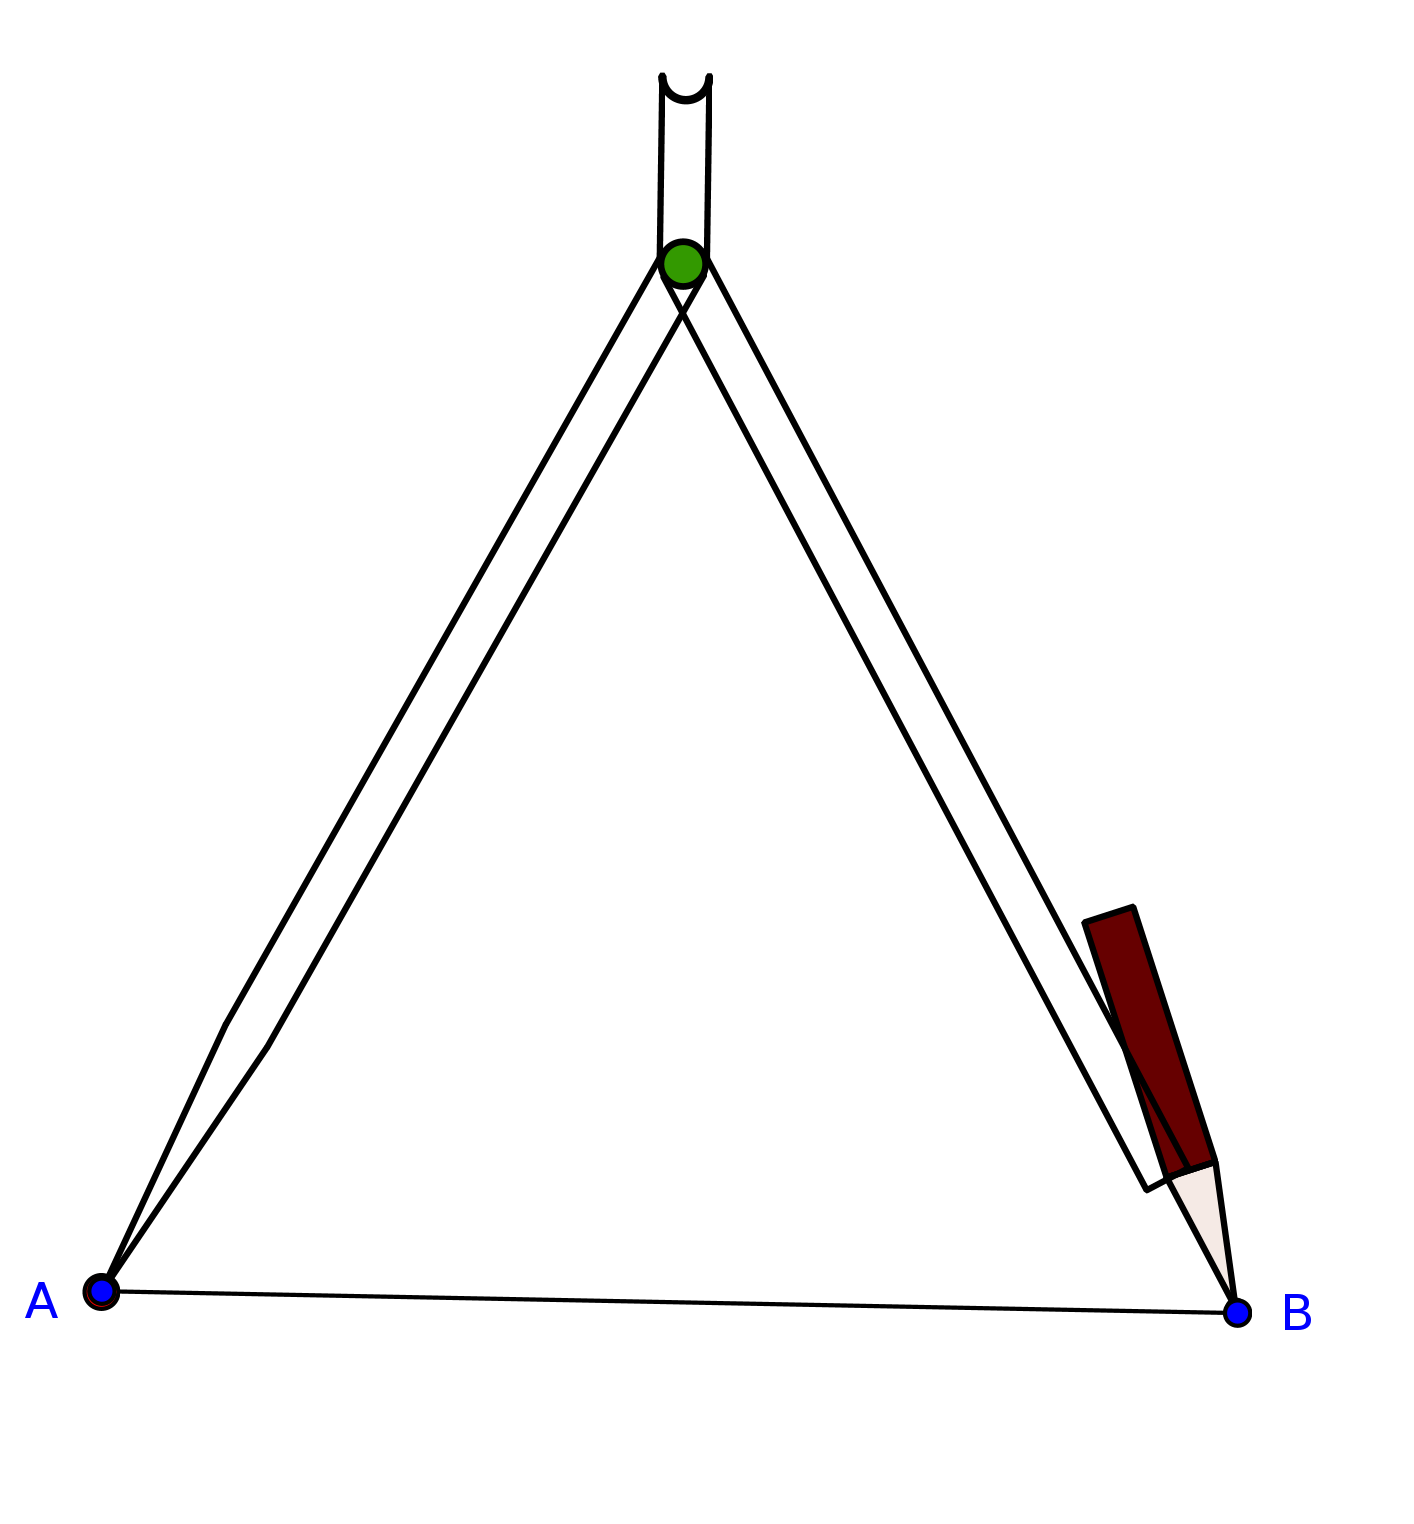
\includegraphics[scale=0.4]{./compas1.png}
 % compas1.png: 1414x1524 pixel, 300dpi, 11.97x12.90 cm, bb=0 0 339 366
}{Segmento dado}{segd}
 \end{figura}
\hfill
 \begin{figura}{
 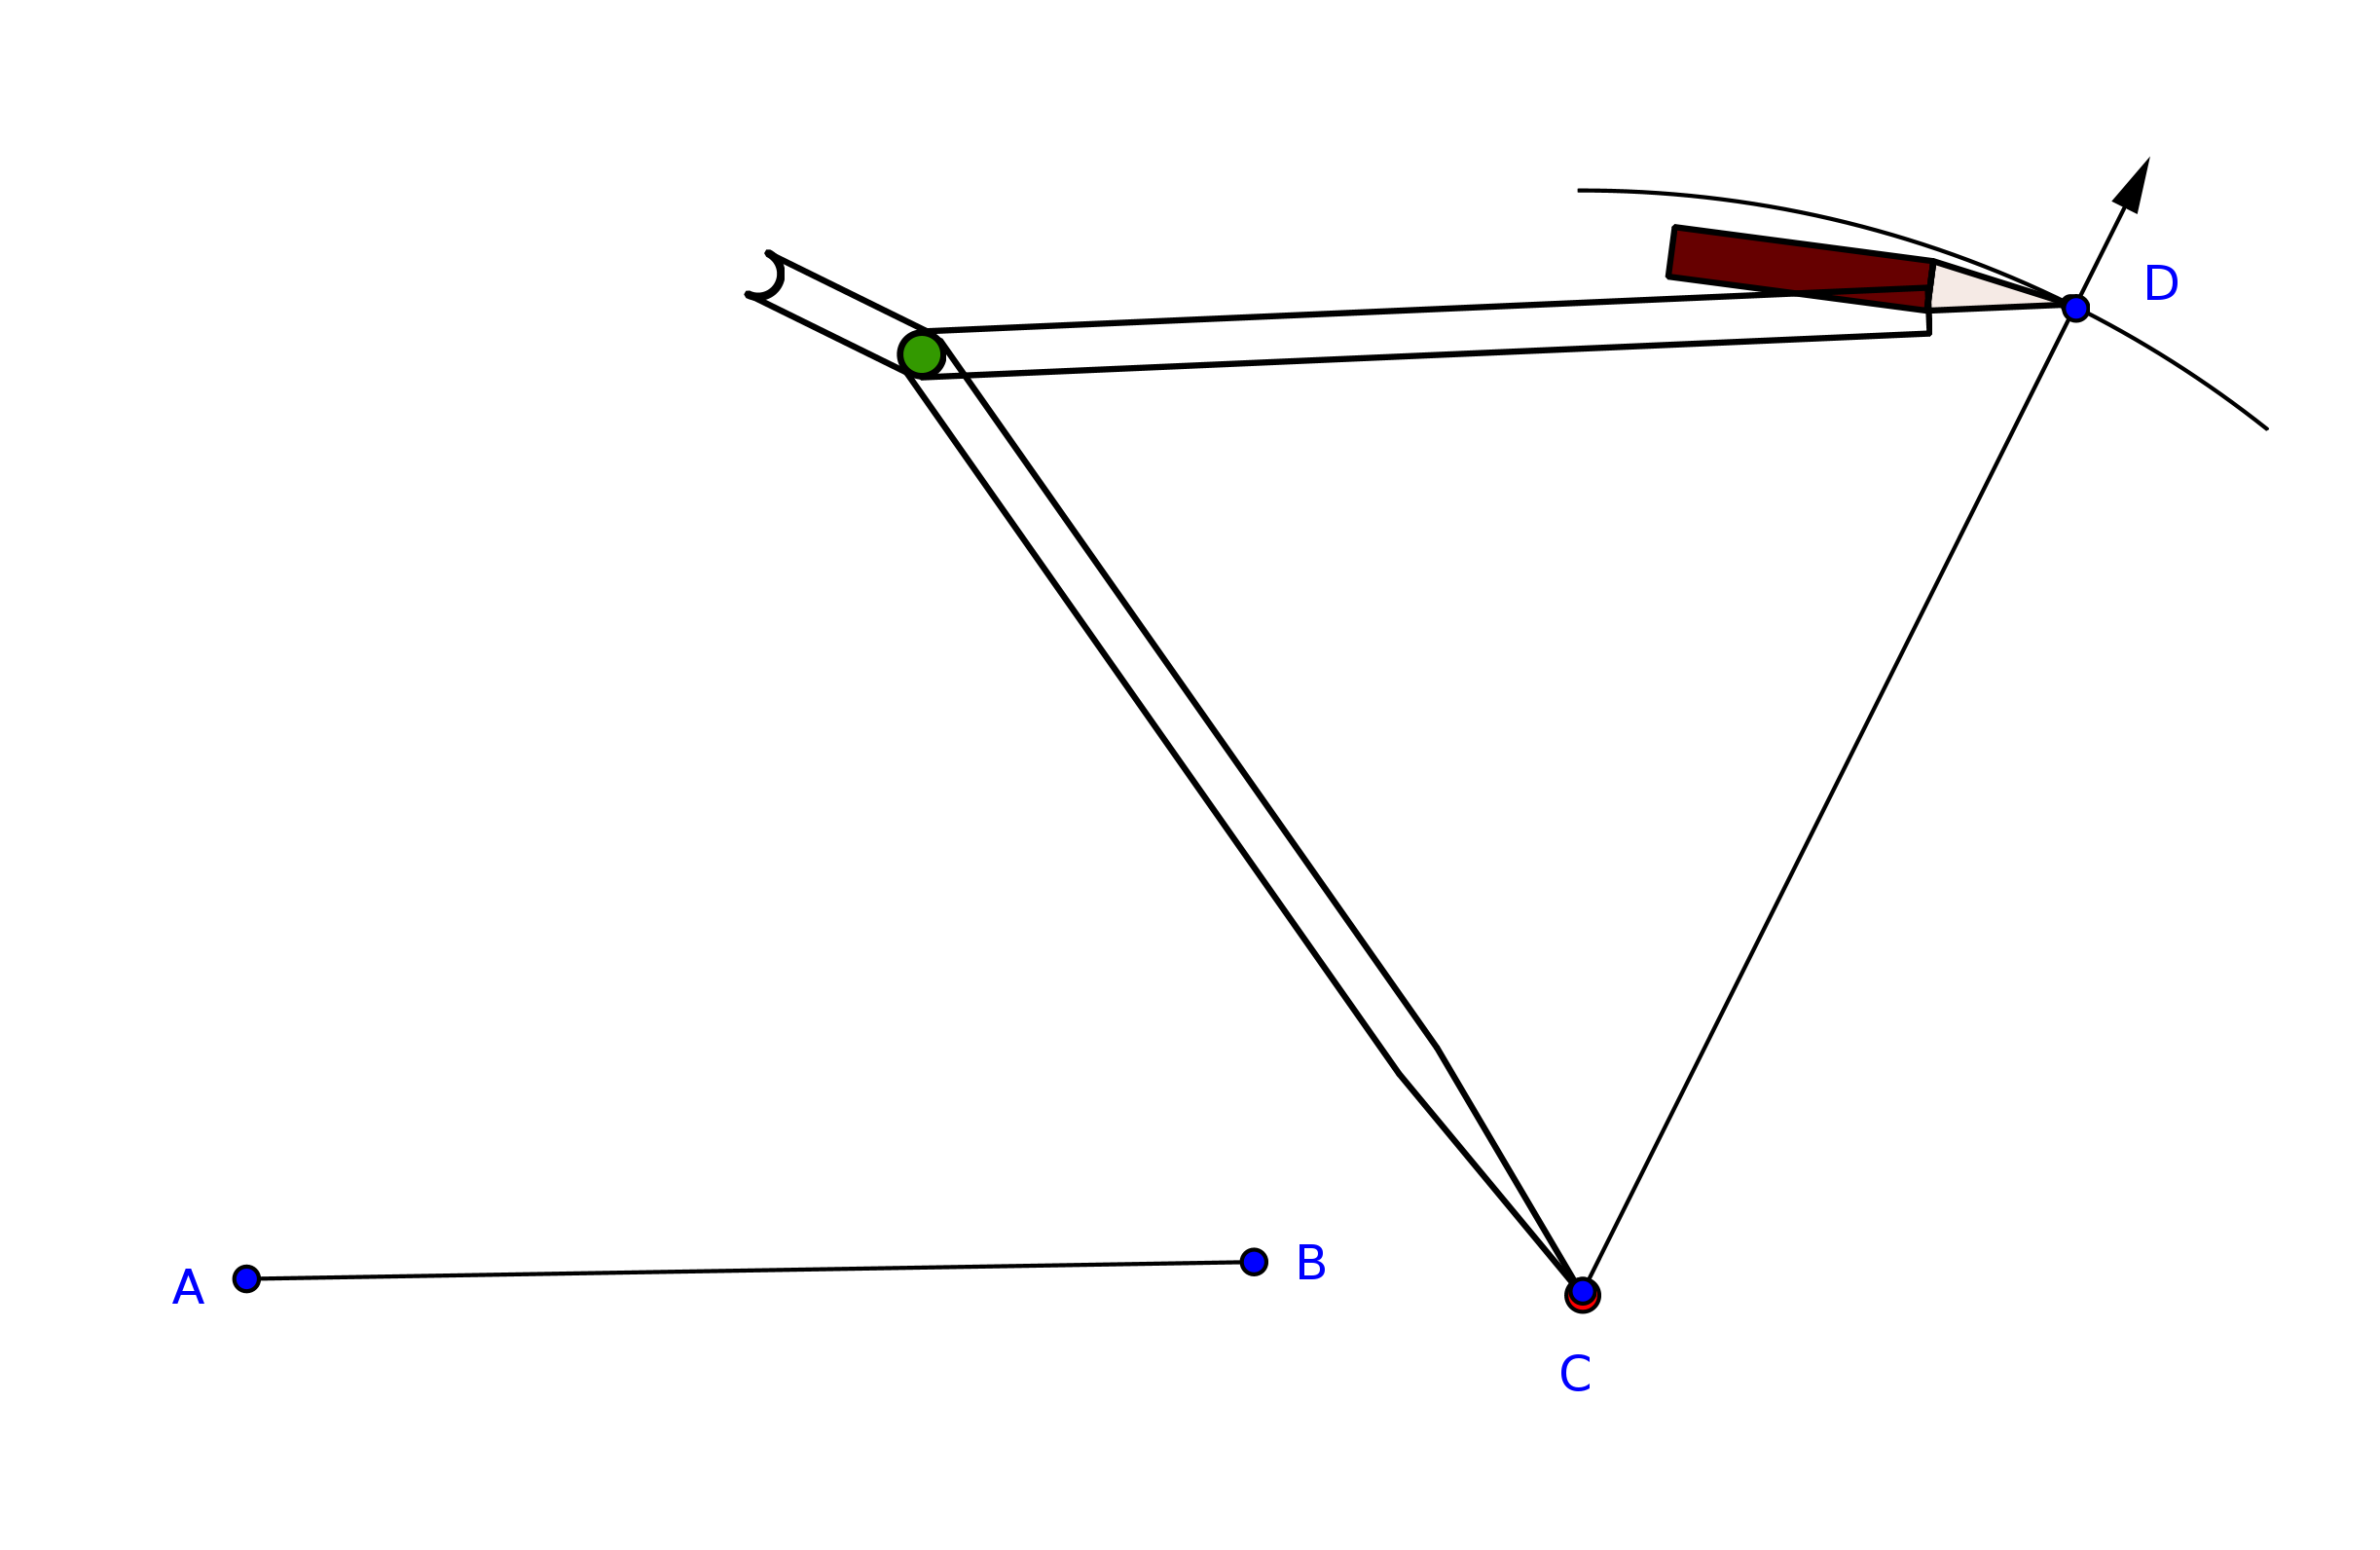
\includegraphics[scale=0.4]{./compas2.png}
 % compas1.png: 1414x1524 pixel, 300dpi, 11.97x12.90 cm, bb=0 0 339 366
}{Segmento duplicado}{segdp}
\end{figura}
De acuerdo con la construcción los segmentos $AB$ y $CD$ de la figura(\ref{segdp})
son congruentes.
\begin{ejemplo}{Un triángulo es un polígono de tres lados, usando esta definición. Construya
Un triángulo con dos lados congruentes.}
 \end{ejemplo}
\solucion En el triángulo de la figura(\ref{trii}) los lados $AB$ y $AC$ son congruentes.
\begin{figura}{
\definecolor{qqqqff}{rgb}{0,0,1}
\begin{tikzpicture}[font=\fontsize{7}{7}\selectfont,scale=1.9,line cap=round,line join=round,>=triangle 45,x=1.0cm,y=1.0cm]
\clip(2.21,0.88) rectangle (6.59,4.32);
\draw [line width=1.2pt,->] (2.98,2.28) -- (5.17,3.6);
\draw [line width=1.2pt,->] (2.98,2.28) -- (6.07,1.49);
\draw [line width=1.2pt,shift={(2.98,2.28)}] plot[domain=-0.74:0.85,variable=\t]({1*1.64*cos(\t r)+0*1.64*sin(\t r)},{0*1.64*cos(\t r)+1*1.64*sin(\t r)});
\draw (2.98,2.28)-- (4.57,1.87);
\draw (3.62,3) node[anchor=north west] {a};
\draw [line width=1.2pt](4.57,1.87)-- (4.39,3.13);
\fill [color=qqqqff] (2.98,2.28) circle (2.0pt);
\draw[color=qqqqff] (2.88,2.28) node {$A$};
\fill [color=qqqqff] (4.57,1.87) circle (1.5pt);
\draw[color=qqqqff] (4.66,1.75) node {$B$};
\fill [color=qqqqff] (4.39,3.13) circle (1.5pt);
\draw[color=qqqqff] (4.41,3.31) node {$C$};
\draw[color=black] (3.77,2) node {$a$};
\draw[color=black] (4.37,2.51) node {$b$};
\end{tikzpicture}}{Triángulo isósceles.}{trii}
\end{figura}

\begin{construccion}{
Para construir dos ángulos congruentes se realizan los siguientes pasos:
\begin{lista}
 \item Dado un ángulo.
\item Se traza un arco con centro en el vértice que corte a los otros dos lados,
y se marcan los puntos de intersección.
\item Se construye un rayo, para que sea un lado del ángulo a duplicado.
\item Con la misma abertura del compás se traza un arco sobre el rayo, con centro
en el origen del rayo.
\item Coloque la puntas del compás sobre los puntos de intersección del arco y los lados del ángulo dado.
\item En el punto de intersección del arco y el rayo trace un nuevo arco centrado en este punto
 y con la misma abertura del compás del paso anterior.
\item una el punto de interseccion de los arcos trazados sobre el rayo y el
origen de este.
\end{lista}
}{Ángulos congruentes}
\begin{figura}{
\definecolor{xdxdff}{rgb}{0.49,0.49,1}
\definecolor{qqqqff}{rgb}{0,0,1}
\begin{tikzpicture}[font=\fontsize{7}{7}\selectfont,scale=1.9,line cap=round,line join=round,>=triangle 45,x=1.0cm,y=1.0cm]
\clip(2.28,0.61) rectangle (11.05,4.48);
\draw [line width=1.2pt,->] (2.98,2.28) -- (5.17,3.6);
\draw [line width=1.2pt,->] (2.98,2.28) -- (6.07,1.49);
\draw [line width=1.2pt,->] (7.13,1.33) -- (10.63,1.32);
\draw [line width=1.2pt,shift={(2.98,2.28)}] plot[domain=-0.74:0.85,variable=\t]({1*1.64*cos(\t r)+0*1.64*sin(\t r)},{0*1.64*cos(\t r)+1*1.64*sin(\t r)});
\draw [line width=1.2pt](2.98,2.28)-- (4.57,1.87);
\draw [line width=1.2pt,shift={(7.13,1.33)}] plot[domain=0:1.28,variable=\t]({1*1.64*cos(\t r)+0*1.64*sin(\t r)},{0*1.64*cos(\t r)+1*1.64*sin(\t r)});
\draw (7.8,1.29) node[anchor=north west] {a};
\draw [line width=1.2pt] (4.57,1.87)-- (4.39,3.13);
\draw [line width=1.2pt,shift={(8.77,1.33)}] plot[domain=1.96:3.43,variable=\t]({1*1.26*cos(\t r)+0*1.26*sin(\t r)},{0*1.26*cos(\t r)+1*1.26*sin(\t r)});
\draw [line width=1.2pt](8.77,1.33)-- (8.28,2.49);
\draw (8.36,2) node[anchor=north west] {b};
\draw [line width=1.2pt,shift={(8.77,1.33)}] plot[domain=1.63:3.25,variable=\t]({1*1.27*cos(\t r)+0*1.27*sin(\t r)},{0*1.27*cos(\t r)+1*1.27*sin(\t r)});
\draw [line width=1.2pt,line width=1.2pt,->] (7.13,1.33) -- (9.03,3.24);
\fill [color=qqqqff] (2.98,2.28) circle (1.5pt);
\draw[color=qqqqff] (2.78,2.28) node {$A$};
\fill [color=qqqqff] (4.57,1.87) circle (1.5pt);
\draw[color=qqqqff] (4.66,1.75) node {$B$};
\fill [color=qqqqff] (4.39,3.13) circle (1.5pt);
\draw[color=qqqqff] (4.41,3.31) node {$C$};
\fill [color=qqqqff] (7.13,1.33) circle (1.5pt);
\draw[color=qqqqff] (7.02,1.38) node {$D$};
\draw[color=black] (3.77,2) node {$a$};
\fill [color=xdxdff] (8.77,1.33) circle (1.5pt);
\draw[color=xdxdff] (8.83,1.2) node {$E$};
\draw[color=black] (4.37,2.51) node {$b$};
\fill [color=xdxdff] (8.28,2.49) circle (1.5pt);
\draw[color=xdxdff] (8.24,2.34) node {$F$};
\end{tikzpicture}}{Ángulos congruentes}{angc}
 \end{figura}
\end{construccion}
\begin{ejemplo}{Construya un triángulo con dos ángulos congruentes. }
\begin{figura}{
\definecolor{xdxdff}{rgb}{0.49,0.49,1}
\definecolor{qqqqff}{rgb}{0,0,1}
\begin{tikzpicture}[font=\fontsize{8}{8}\selectfont,scale=3.0,line cap=round,line join=round,>=triangle 45,x=1.0cm,y=1.0cm]
\clip(1.34,-0.23) rectangle (4.12,1.92);
\draw [line width=1.2pt,->] (1.61,0.24) -- (2.79,1.76);
\draw [line width=1.2pt,->] (1.61,0.24) -- (4.04,0.24);
\draw [line width=1.2pt,shift={(1.61,0.24)}] plot[domain=0:1.23,variable=\t]({1*0.82*cos(\t r)+0*0.82*sin(\t r)},{0*0.82*cos(\t r)+1*0.82*sin(\t r)});
\draw [line width=1.2pt](1.61,0.24)-- (2.43,0.24);
\draw [line width=1.2pt,shift={(3.66,0.24)}] plot[domain=1.9:3.14,variable=\t]({1*0.82*cos(\t r)+0*0.82*sin(\t r)},{0*0.82*cos(\t r)+1*0.82*sin(\t r)});
\draw [line width=1.2pt](2.43,0.24)-- (2.11,0.89);
\draw [line width=1.2pt,shift={(2.43,0.24)}] plot[domain=2.03:2.39,variable=\t]({1*0.72*cos(\t r)+0*0.72*sin(\t r)},{0*0.72*cos(\t r)+1*0.72*sin(\t r)});
\draw [line width=1.2pt,shift={(2.43,0.24)}] plot[domain=1.77:2.5,variable=\t]({1*0.73*cos(\t r)+0*0.73*sin(\t r)},{0*0.73*cos(\t r)+1*0.73*sin(\t r)});
\draw [line width=1.2pt,shift={(2.83,0.23)}] plot[domain=0.01:1.39,variable=\t]({1*0.71*cos(\t r)+0*0.71*sin(\t r)},{0*0.71*cos(\t r)+1*0.71*sin(\t r)});
\draw [line width=1.2pt](3.66,0.24)-- (2.49,1.74);
\draw [line width=1.2pt,->] (3.66,0.24) -- (2.57,0.24);
\draw [line width=1.2pt,->] (2.81,1.34) -- (2.47,1.77);
\fill [color=qqqqff] (1.61,0.24) circle (1.0pt);
\draw[color=qqqqff] (1.48,0.24) node {$A$};
\fill [color=xdxdff] (2.43,0.24) circle (1.0pt);
\draw[color=xdxdff] (2.44,0.16) node {$B$};
\fill [color=xdxdff] (3.66,0.24) circle (1.0pt);
\draw[color=xdxdff] (3.67,0.17) node {$D$};
\fill [color=qqqqff] (2.11,0.89) circle (1.0pt);
\draw[color=qqqqff] (2.1,1.03) node {$C$};
\draw[color=black] (2.04,0.19) node {$a$};
\draw[color=black] (2.19,0.54) node {$b$};
\fill [color=qqqqff] (2.83,0.23) circle (1.0pt);
\draw[color=qqqqff] (2.83,0.14) node {$E$};
\fill [color=qqqqff] (3.15,0.88) circle (1.0pt);
\draw[color=qqqqff] (3.17,1.02) node {$F$};
\fill [color=qqqqff] (2.63,1.56) circle (1.0pt);
\draw[color=qqqqff] (2.62,1.71) node {$G$};
\end{tikzpicture}}{Triángulo con dos ángulos congruentes}{triaa}
 \end{figura}
En el \triangulo $ADG$ los ángulos $ABC$ y $EDF$ son congruentes.
\end{ejemplo}



\begin{construccion}{Para bisecar un ángulo se realizan los siguientes
pasos:
\begin{lista}
 \item Dado un segmento
\item Se traza una semi circunferencia con centro en un extremo
del segmento y que lo intersecte en un punto.
\item Se traza una semi circunferencia con centro en el otro extremo, de tal
forma que intersecte al primero.
\item Se traza un segmento con extremos en los puntos de intersección de las semi circunferencias.
\item El punto de intersección de los dos segmentos es el punto medio.
\end{lista}
}{Punto medio de un segmento}
\begin{figura}{\definecolor{uququq}{rgb}{0.25,0.25,0.25}
\definecolor{qqqqff}{rgb}{0,0,1}
\begin{tikzpicture}[font=\fontsize{7}{7}\selectfont,scale=0.3,line cap=round,line join=round,>=triangle 45,x=1.0cm,y=1.0cm]
\clip(-17.82,-11.18) rectangle (19.74,13.88);
\draw [line width=1.2pt] (-5.03,2.12)-- (4.09,2.12);
\draw(-5.03,2.12) circle (9.12cm);
\draw(4.09,2.12) circle (9.11cm);
\draw [line width=1.2pt,dash pattern=on 5pt off 5pt] (-0.46,10.01)-- (-0.46,-5.78);
\draw [->] (3.92,-2.83) -- (-0.46,2.12);
\draw (3.16,-2.86) node[anchor=north west] {Punto medio};
\fill [color=qqqqff] (-5.03,2.12) circle (1.5pt);
\draw[color=qqqqff] (-6.69,2.37) node {$A$};
\fill [color=qqqqff] (4.09,2.12) circle (1.5pt);
\draw[color=qqqqff] (5.28,2.52) node {$B$};
\fill [color=uququq] (-0.46,10.01) circle (1.5pt);
\draw[color=uququq] (-0.63,12.21) node {$D$};
\fill [color=uququq] (-0.46,-5.78) circle (1.5pt);
\draw[color=uququq] (-0.63,-7.7) node {$E$};
\fill [color=uququq] (-0.46,2.12) circle (1.5pt);
\draw[color=uququq] (0.05,3.13) node {$F$};
\end{tikzpicture}}{Punto medio}{pm}
 \end{figura}
\end{construccion}
\begin{definicion}{La bisectriz de de un segmento
es una recta que pasa por el punto medio del segmento. }{Bisectriz de un
segmento}
\end{definicion}
\begin{construccion}{Para construir la bisectriz de un segmento que pasa por un punto
 no alineado con el segmento, se realizan los siguientes pasos.
\begin{lista}
 \item Dado un segmento y un punto no alineado.
 \item Se construye el punto medio del segmento.
 \item la bisectriz es la recta que pasa por el punto no alineado y el puto medio.
\end{lista}
}{Bisectriz de un segmento}
\begin{figura}{
\definecolor{uququq}{rgb}{0.25,0.25,0.25}
\definecolor{qqqqff}{rgb}{0,0,1}
\begin{tikzpicture}[font=\fontsize{7}{7}\selectfont,scale=2.8,line cap=round,line join=round,>=triangle 45,x=1.0cm,y=1.0cm]
\clip(0.47,-1.25) rectangle (3.45,1.12);
\draw [line width=1.2pt](1.68,-0.07)-- (2.66,-0.06);
\draw [line width=1.2pt,shift={(2.66,-0.06)}] plot[domain=3.16:4.97,variable=\t]({1*0.98*cos(\t r)+0*0.98*sin(\t r)},{0*0.98*cos(\t r)+1*0.98*sin(\t r)});
\draw [line width=1.2pt,shift={(1.68,-0.07)}] plot[domain=0.02:1.87,variable=\t]({1*0.98*cos(\t r)+0*0.98*sin(\t r)},{0*0.98*cos(\t r)+1*0.98*sin(\t r)});
\draw [line width=1.2pt,shift={(1.68,-0.07)}] plot[domain=0.02:1.87,variable=\t]({1*0.98*cos(\t r)+0.03*0.98*sin(\t r)},{0.03*0.98*cos(\t r)+-1*0.98*sin(\t r)});
\draw [line width=1.2pt,shift={(2.66,-0.06)}] plot[domain=3.16:4.97,variable=\t]({1*0.98*cos(\t r)+0.03*0.98*sin(\t r)},{0.03*0.98*cos(\t r)+-1*0.98*sin(\t r)});
\draw [line width=1.2pt,dotted] (2.16,0.78)-- (2.19,-0.92);
\draw [line width=1.2pt,->](1.11,0.7)-- (3.17,-0.79);
\draw [line width=1.2pt,->](2.17,-0.07)-- (0.75,0.96);
\fill [color=qqqqff] (1.68,-0.07) circle (1.5pt);
\draw[color=qqqqff] (1.48,-0.06) node {$A$};
\fill [color=qqqqff] (2.66,-0.06) circle (1.5pt);
\draw[color=qqqqff] (2.8,-0.01) node {$B$};
\fill [color=uququq] (2.16,0.78) circle (1.5pt);
\draw[color=uququq] (2.38,0.8) node {$C$};
\fill [color=uququq] (2.19,-0.92) circle (1.5pt);
\draw[color=uququq] (1.9,-0.83) node {$D$};
\fill [color=qqqqff] (1.11,0.7) circle (1.5pt);
\draw[color=qqqqff] (1.18,0.82) node {$P$};
\fill [color=uququq] (2.17,-0.07) circle (1.5pt);
\draw[color=uququq] (2.25,0.06) node {$E$};
%\draw[color=black] (2.09,-0.1) node {$e$};
\end{tikzpicture}}{Bisectriz de un segmento}{bisecseg}
\end{figura}

\end{construccion}
\begin{definicion}{La bisectriz de un ángulo es la recta que pasa por el vértice
de un ángulo y forma dos ángulos congruentes}{Bisectriz de un ángulo}
 \end{definicion}
\begin{construccion}{Para bisecar un ángulo se realiza el siguiente
procedimiento:
\begin{lista}
 \item dado un ángulo.
 \item Se traza un arco con centro en el vértice del ángulo que corte los lados
del ángulo.
 \item En cada punto de intersección se construyen dos arcos de igual radio.
 \item Se determina el punto de intersección de los arcos.
 \item La bisectriz es la recta que pasa por el punto de corte de los arcos y el vértice
del ángulo.
\end{lista}
 }{Bisectriz de un ángulo}
\begin{figura}{\definecolor{uququq}{rgb}{0.25,0.25,0.25}
\definecolor{xdxdff}{rgb}{0.49,0.49,1}
\definecolor{qqqqff}{rgb}{0,0,1}
\begin{tikzpicture}[font=\fontsize{7}{7}\selectfont,scale=0.3, line cap=round,line join=round,>=triangle 45,x=1.0cm,y=1.0cm]
\clip(-16.07,-12.85) rectangle (12.77,12.89);
\draw [line width=1.2pt](-10.55,-2.33)-- (3.23,9.71);
\draw [line width=1.2pt](-10.55,-2.33)-- (8.23,-3.99);
\draw [line width=1.2pt,shift={(-10.55,-2.33)},line width=1.2pt,dash pattern=on 5pt off 5pt]  plot[domain=-0.09:0.72,variable=\t]({1*10.94*cos(\t r)+0*10.94*sin(\t r)},{0*10.94*cos(\t r)+1*10.94*sin(\t r)});
\draw [line width=1.2pt](0.35,-3.29) circle (6.09cm);
\draw [line width=1.2pt](0.35,-3.29)-- (-5.71,-2.75);
\draw [line width=1.2pt](-2.42,4.77) circle (6.09cm);
\draw [line width=1.2pt,->] (-10.55,-2.33) -- (3.23,9.71);
\draw [line width=1.2pt,->] (-10.55,-2.33) -- (8.23,-3.99);
\draw [line width=1.2pt,->] (0.35,-3.29) -- (-5.71,-2.75);
\draw (-2.3,-3.31) node[anchor=north west] {r};
\draw (-5.17,5.7) node[anchor=north west] {r};
\draw [line width=1.2pt,->] (-2.42,4.77) -- (-8.05,7.08);
\draw [line width=1.2pt,domain=-16.07:12.77] plot(\x,{(--15.55--4.48*\x)/13.62});
\fill [color=qqqqff] (-10.55,-2.33) circle (1.5pt);
\draw[color=qqqqff] (-11.83,-1.34) node {$A$};
\fill [color=qqqqff] (3.23,9.71) circle (1.5pt);
\draw[color=qqqqff] (3.84,10.7) node {$B$};
\fill [color=qqqqff] (8.23,-3.99) circle (1.5pt);
\draw[color=qqqqff] (8.83,-3.01) node {$D$};
\fill [color=xdxdff] (0.35,-3.29) circle (1.5pt);
\draw[color=xdxdff] (0.35,-4.29) node {$E$};
\fill [color=xdxdff] (-2.42,4.77) circle (1.5pt);
\draw[color=xdxdff] (-2.37,6.08) node {$F$};
\fill [color=xdxdff] (-5.71,-2.75) circle (1.5pt);
\draw[color=xdxdff] (-6.76,-3.92) node {$H$};
\fill [color=xdxdff] (-8.05,7.08) circle (1.5pt);
\fill [color=uququq] (3.07,2.15) circle (1.5pt);
\draw[color=uququq] (4.37,3.88) node {$J$};
\fill [color=uququq] (-5.14,-0.67) circle (1.5pt);
\draw[color=uququq] (-5.4,0.93) node {$K$};
%\draw[color=black] (-26.37,-6.34) node {$g$};
\end{tikzpicture}}{Bisectriz del ángulo}{biseca}
\end{figura}
\end{construccion}
\begin{ejemplo}{Construya una flor de 4 pétalos bisecando en ángulo  de 90 grados para cada
pétalo.}
\solucion
\begin{figura}{
\definecolor{qqqqff}{rgb}{0,0,1}
\definecolor{uququq}{rgb}{0.25,0.25,0.25}
\definecolor{ttttff}{rgb}{0.2,0.2,1}
\definecolor{ffttzz}{rgb}{1,0.2,0.6}
\begin{tikzpicture}[font=\fontsize{7}{7}\selectfont,scale=3.0,line cap=round,line join=round,>=triangle 45,x=1.0cm,y=1.0cm]
\clip(-0.09,-0.43) rectangle (3.88,2.26);
\draw (0.64,0.9) node[anchor=north west] {$l_1$};
\draw [line width=1.2pt,dotted] (0.49,0.88)-- (3.47,0.86);
\draw [line width=1.2pt,dash pattern=on 1pt off 1pton 2pt off 4pt,color=ttttff,fill=ttttff,fill opacity=0.15] (1.96,0.85) circle (0.57cm);
\draw [line width=1.2pt,dash pattern=on 1pt off 1pt on 2pt off 4pt,color=ffttzz,fill=ffttzz,fill opacity=0.05] (1.39,0.87) circle (1.14cm);
\draw [line width=1.2pt,dash pattern=on 1pt off 1pt on 2pt off 4pt,color=ffttzz,fill=ffttzz,fill opacity=0.05] (2.53,0.86) circle (1.14cm);
\draw [line width=1.2pt,dotted] (1.97,1.86)-- (1.95,-0.12);
\draw [line width=1.2pt,shift={(1.39,0.87)}] plot[domain=-1.58:1.56,variable=\t]({1*0.57*cos(\t r)+0*0.57*sin(\t r)},{0*0.57*cos(\t r)+1*0.57*sin(\t r)});
\draw [line width=1.2pt,shift={(1.96,0.3)}] plot[domain=-0.01:3.13,variable=\t]({1*0.57*cos(\t r)+0*0.57*sin(\t r)},{0*0.57*cos(\t r)+1*0.57*sin(\t r)});
\draw [line width=1.2pt,shift={(1.96,1.44)}] plot[domain=3.13:6.28,variable=\t]({1*0.57*cos(\t r)+0*0.57*sin(\t r)},{0*0.57*cos(\t r)+1*0.57*sin(\t r)});
\draw [line width=1.2pt,shift={(2.53,0.86)}] plot[domain=1.56:4.7,variable=\t]({1*0.57*cos(\t r)+0*0.57*sin(\t r)},{0*0.57*cos(\t r)+1*0.57*sin(\t r)});
\fill [color=ffttzz] (2.53,0.86) circle (1.0pt);
\draw[color=ffttzz] (2.59,0.96) node {$B$};
\fill [color=ffttzz] (1.39,0.87) circle (1.0pt);
\draw[color=ffttzz] (1.32,0.79) node {$C$};
\fill [color=uququq] (1.97,1.86) circle (1.0pt);
\draw[color=uququq] (2.09,1.88) node {$F$};
\fill [color=uququq] (1.95,-0.12) circle (1.0pt);
\draw[color=uququq] (1.79,-0.09) node {$G$};
\fill [color=uququq] (1.96,1.42) circle (1.0pt);
\draw[color=uququq] (2.03,1.51) node {$H$};
\fill [color=uququq] (1.95,0.28) circle (1.0pt);
\draw[color=uququq] (1.99,0.38) node {$I$};
\fill [color=uququq] (1.39,1.44) circle (1.0pt);
\fill [color=uququq] (2.53,1.44) circle (1.0pt);
\fill [color=uququq] (2.53,0.29) circle (1.0pt);
\fill [color=uququq] (1.38,0.3) circle (1.0pt);
\fill [color=qqqqff] (1.96,0.87) circle (1.0pt);
\draw[color=qqqqff] (2.02,0.97) node {$P$};
\end{tikzpicture}}{Flor de cuatro pétalos.}{f4pet}
\end{figura}

\end{ejemplo}

\begin{construccion}{Dado un punto de una recta.
Para construir construir una recta perpendicular que pase por el punto dados
 se realiza lo siguiente:
\begin{lista}
 \item Dado un punto en una recta.
 \item Trace un arco centrado en el punto dado que corte a la recta
en dos puntos.
 \item Trace dos arcos centrados en cada uno de los puntos de corte del paso
anterior.
 \item Trace la linea perpendicular entre el punto de intersección de los
arcos construidos en el paso anterior y el punto dado.
\end{lista}
}{Recta perpendicular dado un punto en ella}
 \end{construccion}
 \begin{figura}{
\definecolor{qqqqff}{rgb}{0,0,1}
\definecolor{xdxdff}{rgb}{0.49,0.49,1}
\begin{tikzpicture}[font=\fontsize{8}{8}\selectfont,scale=1.3, line cap=round,line join=round,>=triangle 45,x=1.0cm,y=1.0cm]
\clip(0.25,0.58) rectangle (5.98,4.97);
\draw [line width=1pt,shift={(4.67,1.48)}] plot[domain=1.94:3.15,variable=\t]({1*3.21*cos(\t r)+0*3.21*sin(\t r)},{0*3.21*cos(\t r)+1*3.21*sin(\t r)});
\draw [line width=1pt,shift={(1.46,1.45)}] plot[domain=0.01:1.21,variable=\t]({1*3.22*cos(\t r)+0*3.22*sin(\t r)},{0*3.22*cos(\t r)+1*3.22*sin(\t r)});
\draw[line width=1pt, <->] (3.09,0.93)-- (3.03,4.65);
\draw[line width=1pt, <->] (0.48,1.43)-- (5.73,1.5);
\draw [line width=1pt,shift={(3.06,1.47)}] plot[domain=0.01:3.15,variable=\t]({1*1.61*cos(\t r)+0*1.61*sin(\t r)},{0*1.61*cos(\t r)+1*1.61*sin(\t r)});
\fill [color=xdxdff] (4.67,1.48) circle (1.5pt);
\draw[color=xdxdff] (4.77,1.66) node {$B$};
\fill [color=xdxdff] (1.46,1.45) circle (1.5pt);
\draw[color=xdxdff] (1.30,1.68) node {$A$};
\fill [color=qqqqff] (3.07,1.47) circle (1.5pt);
\draw[color=qqqqff] (3.18,1.63) node {$P$};
\fill [color=qqqqff] (3.03,4.24) circle (1.5pt);
\draw[color=qqqqff] (3.20,4.51) node {$C$};
\end{tikzpicture}}{Recta perpendicular}{recpp}
 \end{figura}
\begin{definicion}{La mediatriz de un segmento es la bisectriz perpedicular del segmento}{Mediatriz}
 \begin{figura}{
\definecolor{uququq}{rgb}{0.25,0.25,0.25}
\definecolor{qqqqff}{rgb}{0,0,1}
\begin{tikzpicture}[scale=1.5,font=\fontsize{7}{7}\selectfont,line cap=round,line join=round,>=triangle 45,x=1.0cm,y=1.0cm]
\clip(1.61,-3.8) rectangle (9.06,2.1);
\draw [line width=1pt](4.25,-0.47)-- (6.53,-0.47);
\draw [line width=1pt](4.25,-0.47) circle (2.27cm);
\draw [line width=1pt](6.53,-0.47) circle (2.27cm);
\draw [line width=1pt,<->](5.39,-3.8) -- (5.39,2.1);
\draw (5.55,-2.66) node[anchor=north west] {$l_1$};
\fill [color=qqqqff] (4.25,-0.47) circle (1.0pt);
\draw[color=qqqqff] (4.35,-0.31) node {$A$};
\fill [color=qqqqff] (6.53,-0.48) circle (1.0pt);
\draw[color=qqqqff] (6.63,-0.31) node {$B$};
\fill [color=uququq] (5.38,-2.44) circle (1.0pt);
\draw[color=uququq] (4.95,-2.35) node {$C$};
\fill [color=uququq] (5.4,1.49) circle (1.0pt);
\draw[color=uququq] (4.89,1.55) node {$D$};
\end{tikzpicture}}{Mediatriz de un segmento}{mediatriz}
\end{figura}
\end{definicion}
\begin{construccion}{Dado un punto y una recta no alineados para trazar
 una recta perpendicular que contiene al punto. Se realiza lo siguiente:
\begin{lista}
 \item Dada una recta y un punto no alineado.
\item Centrados en el punto dado trace dos arcos de igual radio
 que intersecten la recta.
\item Centrados en los puntos de intersección del paso anterior
trace dos arcos de igual radio, en lado opuesto de la recta al punto dado.
\item Una el punto de intersección de los arcos del paso anterior y el punto dado.
\end{lista}
}{Rectas perpendiculares}
\begin{figura}{
\definecolor{fftttt}{rgb}{1,0.2,0.2}
\definecolor{uququq}{rgb}{0.25,0.25,0.25}
\definecolor{ttqqff}{rgb}{0.2,0,1}
\definecolor{qqqqff}{rgb}{0,0,1}
\begin{tikzpicture}[font=\fontsize{8}{8}\selectfont,scale=3.3,line cap=round,line join=round,>=triangle 45,x=1.0cm,y=1.0cm]
\clip(3.2,-1.41) rectangle (7.81,1.14);
\draw [line width=1pt,<->] (3.75,-0.14)-- (6.7,-0.15);
\draw [line width=1pt,shift={(5.26,0.37)},line width=1.2pt,dash pattern=on 1pt off 1pt,color=ttqqff]  plot[domain=3.72:5.78,variable=\t]({1*0.71*cos(\t r)+0*0.71*sin(\t r)},{0*0.71*cos(\t r)+1*0.71*sin(\t r)});
\draw [line width=1pt,line width=1.2pt,dash pattern=on 1pt off 1pt,color=fftttt] (4.78,-0.14) circle (0.71cm);
\draw [line width=1.2pt,dash pattern=on 1pt off 1pt,color=fftttt] (5.75,-0.14) circle (0.71cm);
\draw (3.84,-0.13) node[anchor=north west] {$l_1$};
\draw [->,line width=1.2pt,dash pattern=on 1pt off 1pt,color=ttqqff] (5.26,0.37) -- (5.83,-0.06);
\draw [line width=1pt,->,color=fftttt] (4.78,-0.14) -- (4.33,-0.7);
\draw [line width=1pt,->,color=fftttt] (5.75,-0.14) -- (6.37,-0.49);
\draw (4.63,-0.32) node[anchor=north west] {$r_1$};
\draw (5.98,-0.31) node[anchor=north west] {$r_2$};
\draw [line width=1pt,<->](5.26,0.75)-- (5.26,-0.99);
\draw (5.31,0.74) node[anchor=north west] {$l_2$};
\fill [color=qqqqff] (5.26,0.37) circle (1.0pt);
\draw[color=qqqqff] (5.35,0.39) node {$P$};
\fill [color=uququq] (4.78,-0.14) circle (1.0pt);
\draw[color=uququq] (4.81,-0.08) node {$A$};
\fill [color=uququq] (5.75,-0.14) circle (1.0pt);
\draw[color=uququq] (5.79,-0.21) node {$B$};
\fill [color=uququq] (5.26,0.37) circle (1.0pt);
\fill [color=uququq] (5.26,-0.66) circle (1.0pt);
\end{tikzpicture}}{Rectas Perpendiculares}{rpenpna}
\end{figura}
\end{construccion}
\begin{definicion}{La distancia entre un punto y una recta
es la medida del segmento perpendicular entre el punto y la recta. }{Distancie entre un punto y una recta.}
\end{definicion}
\begin{figura}{\definecolor{fftttt}{rgb}{1,0.2,0.2}
\definecolor{uququq}{rgb}{0.25,0.25,0.25}
\definecolor{ttqqff}{rgb}{0.2,0,1}
\definecolor{qqqqff}{rgb}{0,0,1}
\begin{tikzpicture}[font=\fontsize{8}{8}\selectfont,scale=3.3,line cap=round,line join=round,>=triangle 45,x=1.0cm,y=1.0cm]
\clip(3.2,-1.41) rectangle (7.81,1.14);
\draw [<->,line width=1.2pt](3.75,-0.14)-- (6.7,-0.15);
\draw [shift={(5.26,0.37)},line width=1.2pt,dash pattern=on 1pt off 1pt,color=ttqqff]  plot[domain=3.72:5.78,variable=\t]({1*0.71*cos(\t r)+0*0.71*sin(\t r)},{0*0.71*cos(\t r)+1*0.71*sin(\t r)});
\draw [line width=1.2pt,dash pattern=on 1pt off 1pt,color=fftttt] (4.78,-0.14) circle (0.71cm);
 \draw [line width=1.2pt,dash pattern=on 1pt off 1pt,color=fftttt] (5.75,-0.14) circle (0.71cm);
 \draw (3.84,-0.13) node[anchor=north west] {$l_1$};
 \draw [->,line width=1.2pt,dash pattern=on 1pt off 1pt,color=ttqqff] (5.26,0.37) -- (5.83,-0.06);
 \draw [->,color=fftttt] (4.78,-0.14) -- (4.33,-0.7);
 \draw [->,color=fftttt] (5.75,-0.14) -- (6.37,-0.49);
 \draw (4.63,-0.32) node[anchor=north west] {$r_1$};
 \draw (5.98,-0.31) node[anchor=north west] {$r_2$};
 \draw (5.26,0.37)-- (5.26,-0.66);
 \fill [color=qqqqff] (5.26,0.37) circle (1.0pt);
 \draw[color=qqqqff] (5.35,0.39) node {$P$};
 \fill [color=uququq] (4.78,-0.14) circle (1.0pt);
 \draw[color=uququq] (4.81,-0.08) node {$A$};
\fill [color=uququq] (5.75,-0.14) circle (1.0pt);
\draw[color=uququq] (5.79,-0.21) node {$B$};
%\fill [color=uququq] (5.26,0.37) circle (1.0pt);
 \fill [color=uququq] (5.26,-0.66) circle (1.0pt);
 \draw[color=qqqqff] (5.35,-0.08) node {$C$};
 \fill [color=qqqqff] (5.26,-0.14) circle (1.0pt);
  \draw[line width=1.2pt,color=qqqqff] (5.26,0.39)--(5.26,-0.14);
 \end{tikzpicture}
}{Distancia entre un punto y una recta.}{recpp}
 \end{figura}
\chapter[
     image=def,%genetics-dogs,
     image caption={The global option open right, triggers the typesetting of chapter on odd pages only. There are a  couple of layouts that must be typeset on an even pages.}]%
         %{1}
{Razonamiento en geometr\'ia}
{\begin{itemize}
 \item En este cap\'itulo seguiremos con la construci\'on axiomática de la geometr\'ia
y paralelamente presentaremos construcciones con regla y c\'ompas, que luego al
final de este cap\'itulo empezaremos a demostrar.
\item Del párrafo anterior se nos presenta una duda, ¿Qué es demostrar? 
Podemos considerar la demostración de una proposición $q$ como una cadena finita
de conclusiones que se realizan mediante reglas lógicas y que se forman a partir
de proposiciones verdaderas o supuestamente verdaderas y las cuales nos conducen
a una proposición $p$.
\item La proposición o relación resultante de otras mediante el proceso de la
demostración se llama \texttt{teorema} y este proceso podemos dividirlo
tres partes (figura\ref{demos} ):
\end{itemize}
\begin{lista}
\item  Conocer la proposición que se trata de demostrar. En esta parte es
importante diferenciar muy claramente la información que nos dan (la
hipótesis) de lo que nos solicitan que demostremos (la tesis).
\item Los fundamentos empleados como base de la demostración. Estos fundamentos
   están constituidos por los términos primitivos, las definiciones, los
postulados y las proposiciones o teoremas ya demostrados.
\item  El procedimiento usado para lograr que la proposición quede demostrada
(elegir el método adecuado).
\end{lista}}
\label{chap:2}
\vspace{40pt}
\seccion{Introducci\'on}
\begin{figura}{
\definecolor{zzccff}{rgb}{0.6,0.8,1}
\definecolor{cqcqcq}{rgb}{0.75,0.75,0.75}
\begin{tikzpicture}[scale=1.2,line cap=round,font=\fontsize{7}{7}\selectfont,line
join=round,>=triangle
45,x=1.0cm,y=1.0cm]
%\draw [color=cqcqcq,dash pattern=on 1pt off 1pt, xstep=2.0cm,ystep=2.0cm]
%(-0.27,1.66) grid (12.29,5.02);
\clip(-0.27,1.66) rectangle (12.29,5.02);
\fill[color=zzccff,fill=zzccff,fill opacity=0.1] (0,4) -- (4,4) -- (4,2) --
(0,2) -- cycle;
\fill[color=zzccff,fill=zzccff,fill opacity=0.1] (4.5,3.5) -- (6.5,3.5) --
(6.5,4) -- (7.5,3) -- (6.5,2) -- (6.5,2.5) -- (4.5,2.5) -- cycle;
\fill[color=zzccff,fill=zzccff,fill opacity=0.1] (8,4) -- (12,4) -- (12,2) --
(8,2) -- cycle;
\draw [color=zzccff] (0,4)-- (4,4);
\draw [color=zzccff] (4,4)-- (4,2);
\draw [color=zzccff] (4,2)-- (0,2);
\draw [color=zzccff] (0,2)-- (0,4);
\draw [color=zzccff] (4.5,3.5)-- (6.5,3.5);
\draw [color=zzccff] (6.5,3.5)-- (6.5,4);
\draw [color=zzccff] (6.5,4)-- (7.5,3);
\draw [color=zzccff] (7.5,3)-- (6.5,2);
\draw [color=zzccff] (6.5,2)-- (6.5,2.5);
\draw [color=zzccff] (6.5,2.5)-- (4.5,2.5);
\draw [color=zzccff] (4.5,2.5)-- (4.5,3.5);
\draw [color=zzccff] (8,4)-- (12,4);
\draw [color=zzccff] (12,4)-- (12,2);
\draw [color=zzccff] (12,2)-- (8,2);
\draw [color=zzccff] (8,2)-- (8,4);
\draw (0.61,3.69) node[anchor=north west] {\parbox{3.78 cm}{Términos no
definidos \\ Definiciones 
\\  Postulados \\  Otros  teoremas}};
\draw (1.16,4.54) node[anchor=north west] {Hipótesis};
\draw (4.48,4.52) node[anchor=north west] {Razonamieto lógico};
\draw (9.47,4.57) node[anchor=north west] {Tesis};
\draw (9.31,3.09) node[anchor=north west] {Conclusión};
\draw (4.7,3.36) node[anchor=north west] {\parbox{2.71 cm}{Esquema de 
\\  razonamiento}};
\end{tikzpicture}}{Esquema de una demostración}{demos}
 Para realizar una demostración además de tener las reglas lógicas y el
encadenamiento de proposiciones, también hay que determinar un método o
razona\-miento como expondremos a continuación.
\end{figura}
\vspace{-20pt}
\seccion{Razonamiento inductivo}
El razonamiento inductivo es el proceso mediante el cual se obtienen
conclusiones a partir de nuestras propias observaciones o a partir de ejemplos
particulares, es decir al observar que una acci\'on o propiedad se repite se
concluye en general que esa acci\'on o propiedad siempre es cierta
\begin{ideas}{Es la conclusi\'on que se obtiene a partir de un
\vspace{-20pt}
proceso inductivo}{Conjetura}
\end{ideas}

\begin{ejemplo}{Suponga que una persona mide los lados de cuatro  tri\'angulos
como muestra la figura(\ref{dest})}
\begin{figura}{
\definecolor{qqqqff}{rgb}{0,0,1}
\begin{tikzpicture}[scale=5.0, font=\fontsize{7}{8}\selectfont,line
cap=round,line join=round,>=triangle 45,x=1.0cm,y=1.0cm]
\clip(0.01,-0.13) rectangle (0.97,2.28);
\draw[line width=1.2pt] (0.05,1.19)-- (0.23,1.93);
\draw[line width=1.2pt] (0.23,1.93)-- (0.36,1.17);
\draw[line width=1.2pt] (0.36,1.17)-- (0.05,1.19);
\draw[line width=1.2pt] (0.11,1.67) node[anchor=north west] {0.77};
\draw[line width=1.2pt] (0.31,1.63) node[anchor=north west] {0.77};
\draw[line width=1.2pt] (0.2,1.13) node[anchor=north west] {0.31};
\draw[line width=1.2pt] (0.44,1.86)-- (0.61,1.12);
\draw[line width=1.2pt] (0.61,1.12)-- (0.91,1.15);
\draw[line width=1.2pt] (0.91,1.15)-- (0.44,1.86);
\draw[line width=1.2pt] (0.5,1.45) node[anchor=north west] {0.76};
\draw[line width=1.2pt] (0.74,1.06) node[anchor=north west] {0.3};
\draw[line width=1.2pt] (0.66,1.65) node[anchor=north west] {0.85};
\draw[line width=1.2pt] (0.06,0.23)-- (0.35,0.77);
\draw[line width=1.2pt] (0.35,0.77)-- (0.4,0.11);
\draw[line width=1.2pt] (0.06,0.23)-- (0.4,0.11);
\draw[line width=1.2pt] (0.38,0.51) node[anchor=north west] {0.67};
\draw[line width=1.2pt] (0.25,0.11) node[anchor=north west] {0.35};
\draw[line width=1.2pt] (0.21,0.68) node[anchor=north west] {0.61};
\draw[line width=1.2pt] (0.54,0.74)-- (0.54,0.11);
\draw[line width=1.2pt] (0.54,0.11)-- (0.81,0.13);
\draw[line width=1.2pt] (0.81,0.13)-- (0.54,0.74);
\draw[line width=1.2pt] (0.67,0.54) node[anchor=north west] {0.35};
\draw[line width=1.2pt] (0.51,0.47) node[anchor=north west] {0.62};
\draw[line width=1.2pt] (0.66,0.1) node[anchor=north west] {0.27};
\fill [color=qqqqff] (0.05,1.19) circle (0.5pt);
\draw[color=qqqqff] (0.04,1.18) node {$A$};
\fill [color=qqqqff] (0.23,1.93) circle (0.5pt);
\draw[color=qqqqff] (0.23,2) node {$B$};
\fill [color=qqqqff] (0.36,1.17) circle (0.5pt);
\draw[color=qqqqff] (0.37,1.14) node {$C$};
\fill [color=qqqqff] (0.44,1.86) circle (0.5pt);
\draw[color=qqqqff] (0.44,1.95) node {$D$};
\fill [color=qqqqff] (0.61,1.12) circle (0.5pt);
\draw[color=qqqqff] (0.61,1.06) node {$E$};
\fill [color=qqqqff] (0.91,1.15) circle (0.5pt);
\draw[color=qqqqff] (0.92,1.13) node {$F$};
\fill [color=qqqqff] (0.06,0.23) circle (0.5pt);
\draw[color=qqqqff] (0.05,0.25) node {$G$};
\fill [color=qqqqff] (0.35,0.77) circle (0.5pt);
\draw[color=qqqqff] (0.36,0.83) node {$H$};
\fill [color=qqqqff] (0.4,0.11) circle (0.5pt);
\draw[color=qqqqff] (0.41,0.1) node {$I$};
\fill [color=qqqqff] (0.54,0.74) circle (0.5pt);
\draw[color=qqqqff] (0.53,0.81) node {$J$};
\fill [color=qqqqff] (0.54,0.11) circle (0.5pt);
\draw[color=qqqqff] (0.53,0.08) node {$K$};
\fill [color=qqqqff] (0.81,0.13) circle (0.5pt);
\draw[color=qqqqff] (0.82,0.15) node {$L$};
\end{tikzpicture}}{Desigualdad triangular}{dest}
\end{figura}
De los cuatro tri\'angulos podemos concluir que la suma de las longitudes de dos
lados siempre es menor que la longitud del tercer lado.
 \end{ejemplo}
\subsection{M\'etodo del contraejemplo}
Hay ocasiones donde despu\'es de un razonamiento inductivo obtenemos una
conjetura que no se cumple para todos los casos, es decir obtenemos una
generalizaci\'on falsa, entonces para indicar que esa generalizaci\'on es falsa
buscamos un ejemplo donde no se cumpla la acci\'on o la propiedad.
\begin{ideas}{Es el m\'etodo que se usa para demostrar que una
generalizaci\'on es falsa, utilizando un ejemplo que la
contradiga.}{Contraejmplo}
\end{ideas}
\begin{ejemplo}{Si un cuadril\'atero tiene sus diagonales perpendiculares,
entonces es un rombo.}
\begin{figura}{
\definecolor{qqwuqq}{rgb}{0,0.39,0}
\definecolor{uququq}{rgb}{0.25,0.25,0.25}
\definecolor{xdxdff}{rgb}{0.49,0.49,1}
\definecolor{qqqqff}{rgb}{0,0,1}
\begin{tikzpicture}[scale=0.7,font=\fontsize{8}{9}\selectfont, cap=round,line
join=round,>=triangle 45,x=1.0cm,y=1.0cm,line width=1.2pt]
\clip(-3.28,-2.66) rectangle (1.6,11.45);
\draw[color=qqwuqq,fill=qqwuqq,fill opacity=0.1] (-0.33,4.17) -- (-0.33,4.34) --
(-0.51,4.34) -- (-0.5,4.17) -- cycle;
\draw (-0.53,9.97)-- (-0.48,-1.04);
\draw (-2.96,4.16)-- (-0.53,9.97);
\draw (-0.53,9.97)-- (1.05,4.18);
\draw (1.05,4.18)-- (-0.48,-1.04);
\draw (-0.48,-1.04)-- (-2.96,4.16);
\draw (-1.92,8.12) node[anchor=north west] {6.29};
\draw (0.22,8.34) node[anchor=north west] {6};
\draw (-2.96,4.16)-- (1.05,4.18);
\fill [color=qqqqff] (-0.53,9.97) circle (1.5pt);
\draw[color=qqqqff] (-0.52,10.58) node {$A$};
\fill [color=qqqqff] (-0.48,-1.04) circle (1.5pt);
\draw[color=qqqqff] (-0.46,-1.47) node {$B$};
\fill [color=qqqqff] (1.05,4.18) circle (1.5pt);
\draw[color=qqqqff] (1.12,4.65) node {$C$};
\fill [color=xdxdff] (-2.96,4.16) circle (1.5pt);
\draw[color=xdxdff] (-2.96,3.23) node {$D$};
\fill [color=uququq] (-0.5,4.17) circle (1.5pt);
\draw[color=qqwuqq] (-0.12,4.94) node {$\alpha = 90$};
\end{tikzpicture}}{Cometa}{com}
 \end{figura}
En el cuadril\'atero podemos observar que $AD=6.29$ y $AC=6$ y por definici\'on
de rombo el cuadril\'atero $ABCD$ no puede ser un rombo porque no tiene sus
lados congruentes.
\end{ejemplo}
\seccion{Razonamiento deductivo}
El método deductivo consiste en partir de un número reducido de información
(hipótesis) y mediante un proceso lógico deducir otros conocimientos o
proposiciones nuevas.
Para profundizar y entender este método explicaremos a continuación cuales son
los procesos lógicos.
\subsection{Tipos de proposiciones lógicas}
En este curso casi siempre trabajaremos con proposiciones compuestas, es decir
una proposici\'on que esta formada por un conjunto de proposiciones, unidas por
operadores l\'ogicos llamados conectores:\\ Esos conectores son
\begin{lista}
\item $\sim$ , es una proposici\'on simple a la cual se le cambia el valor de
verdad. La proposici\'on se llama nagaci\'on.
\setlength{\parindent}{-25pt}
\begin{ejemplo}{La negación de la proposición \textquotedblleft Los ángulos
$\angle\alpha$ y $\angle\beta$ son rectos\textquotedblright\, es:\\
\textquotedblleft El ángulo $\angle\alpha$ no es recto o el ángulo
$\angle\beta$ no es recto\textquotedblright.}
\end{ejemplo}
 \item $\vee$ , a la proposici\'on compuesta formada por este conectivo que se
lee "o``, se llama disyunci\'on.
\begin{ejemplo}{
 Un cuadril\'atero es un polígono con cuatro lados o cuatro v\'ertices.}
\end{ejemplo}

\item $\wedge$ , la proposici\'on resultante se llama conjunci\'on y el conector
se lee " y ''
\begin{ejemplo}{Un polígono regular tiene los ángulos interiores y sus lados
congruentes.}
 \end{ejemplo}
\item $ \mbox{si}\cdots , \mbox{entonces } \cdots$, la proposic\'on resultante
se llama condicional.
\begin{ejemplo}{Dos rectas que no se intersecan son paralelas o alabeadas}
 Est\'a proposición es de la forma $p \rightarrow \left( q \vee r\right) $
\end{ejemplo}
\item $\cdots \mbox{si y s\'olo si} \cdots$, a la proposic\'on resultante se le
llama bicondicional.
\end{lista}
Vamos a hablar un poco de las dos \'ultimas proposiciones:
La condicional es una proposici\'on que se denota de la forma $p\longrightarrow
q$, donde $p$ y $q$ son proposiciones que llamaremos, hip\'otesis y conclusi\'on
respectivamente.
Por ejemplo
\begin{ejemplo}{ Si un tri\'angulo tiene un \'angulo recto, entonces es un
tri\'angulo rect\'angulo.}
En este caso la hip\'otesis es : el tri\'angulo es rect\'angulo y la
conclusi\'on es: el tri\'angulo es rect\'angulo.
\end{ejemplo}
La bicondicional se denota $p\longleftrightarrow q$, y se puede descomponer en
la conjunci\'on de dos condicionales, as\'i: $ p\longrightarrow
q \wedge q\longrightarrow p$.
\begin{ejemplo}{Dos rectas son paralelas si y sólo si sus ángulos alternos
internos formados por una transversal son congruentes}
en este ejemplo $p$\ es: Dos rectas son paralelas.\\
$q$\ es: Los ángulos formados por una transversal son congruentes.   
\end{ejemplo}

\nota\ Para saber el valor de verdad  proposición compuesta se utilizan las definiciones
 organizadas en la siguiente tabla:
\[%
\begin{tabular}
[c]{llllll}%
$ p$ &$q$ & $p\wedge q$ & $p\vee q$ & $p\rightarrow q$ &
$p\leftrightarrow q$\\
\multicolumn{1}{c}{V}&\multicolumn{1}{c}{V} & \multicolumn{1}{c}{V} & \multicolumn{1}{c}{V} &
\multicolumn{1}{c}{V} & \multicolumn{1}{c}{V}\\
\multicolumn{1}{c}{V}&\multicolumn{1}{c}{F} & \multicolumn{1}{c}{F} & \multicolumn{1}{c}{V} &
\multicolumn{1}{c}{F} & \multicolumn{1}{c}{F}\\
\multicolumn{1}{c}{F}&\multicolumn{1}{c}{V} & \multicolumn{1}{c}{F} & \multicolumn{1}{c}{V} &
\multicolumn{1}{c}{V} & \multicolumn{1}{c}{F}\\
\multicolumn{1}{c}{F}&\multicolumn{1}{c}{F} & \multicolumn{1}{c}{F} & \multicolumn{1}{c}{F} &
\multicolumn{1}{c}{V} & \multicolumn{1}{c}{V}%
\end{tabular}
\]
Con la condicional y la bicondicional se pueden construir dos tautologías de la
siguiente
manera:
\begin{ideas}{Es una condicional que siempre es verdadera}{Implicaci\'on}
 Por ejemplo:
\end{ideas}
\begin{ejemplo}{ Si un cuadril\'atero tiene dos lados opuestos paralelos,
entonces estos lados son congruentes.}
La figura(\ref{tra}) llamada trapecio tiene los lados $\overline{AB}$ y
$\overline{CD}$ paralelos y no son congruentes. Por tanto esta condicional no es
una implicaci\'on.
\begin{figura}{\definecolor{xdxdff}{rgb}{0.49,0.49,1}
\definecolor{qqqqff}{rgb}{0,0,1}
\begin{tikzpicture}[scale=0.8,font=\fontsize{9}{8}\selectfont,line
cap=round,line join=round,>=triangle 45,x=1.0cm,y=1.0cm,line width=1.2pt]
\clip(-1.07,-1.25) rectangle (5.06,2.06);
\draw (-0.91,-0.76)-- (-0.21,1.43);
\draw (-0.21,1.43)-- (3.48,1.39);
\draw (3.48,1.39)-- (4.77,-0.81);
\draw (4.77,-0.81)-- (-0.91,-0.76);
\draw (1.46,1.50) node[anchor=north west] {3.69};
\draw (1.7,-0.650) node[anchor=north west] {5.69};
\fill [color=qqqqff] (-0.21,1.43) circle (1.5pt);
\draw[color=qqqqff] (-0.40,1.55) node {$A$};
\fill [color=qqqqff] (3.48,1.39) circle (1.5pt);
\draw[color=qqqqff] (3.55,1.7) node {$B$};
\fill [color=xdxdff] (-0.91,-0.76) circle (1.5pt);
\draw[color=xdxdff] (-0.9,-1.1) node {$D$};
\fill [color=xdxdff] (4.77,-0.81) circle (1.5pt);
\draw[color=xdxdff] (4.85,-1.1) node {$E$};
\end{tikzpicture}}{Trapecio}{tra}
\end{figura}
La condicional se denota $p \Longrightarrow q$ y se lee $p$ implica $q$
\end{ejemplo}
\begin{ideas}{Es una bicondicional que siempre es cierta.}{Doble implicaci\'on}
Por ejemplo todas las definiciones son bicondicionales.
\nota\ La doble implicaci\'on se denota  $p \Longleftrightarrow q$ y se dice que
que $p$ y $q$ son proposiciones lógicamente equivalentes
\end{ideas}
\begin{ejemplo}{Analice el valor de verdad de la proposición compuesta%
\[
(p\rightarrow q)\leftrightarrow(\sim q\rightarrow\sim p)
\]
}
\solucion\ 
%
\[%
\begin{tabular}
[c]{ccccccc}%
$p$ & $q$ & $p\rightarrow q$ & $\sim q$ & $\sim p$ & $\sim q\rightarrow\sim p$
& $(p\rightarrow q)\leftrightarrow(\sim q\rightarrow\sim p)$\\
V & V & V & F & F & V & V\\
V & F & F & V & F & F & V\\
F & V & V & F & V & V & V\\
F & F & V & V & V & V & V
\end{tabular}
\ \
\]
Es decir las proposiciones: $p\rightarrow q$ y $\sim
q\rightarrow\sim p$\ son equivalentes. 
 \end{ejemplo}

\begin{ejemplo}{Presentaremos algunos ejemplos de implicaciones y equivalencia
lógicas\label{ej2_11} } 
\begin{enumerate}
\item $\left[  p\wedge\left(  p\rightarrow q\right)  \right]  \Longrightarrow
q$

\item $\left[  \left(  p\rightarrow q\right)  \wedge\sim q\right]
\Longrightarrow\sim p$

\item $\left[  \left(  p\rightarrow q\right)  \wedge\left(  q\rightarrow
r\right)  \right]  \Longrightarrow\left(  p\rightarrow r\right)  $

\item $\left(  p\wedge q\right)  \Longrightarrow p$
\item $\sim\left(  p\wedge q\right)  \Longleftrightarrow\left(  \sim p\vee\sim
q\right)  $

\item $\sim\left(  p\vee q\right)  \Longleftrightarrow\left(  \sim p\wedge\sim
q\right)  $

\item $\left(  p\rightarrow q\right)  \Longleftrightarrow\left(  \sim
q\rightarrow\sim p\right)  $

\item $\left[  p\rightarrow\left(  q\vee r\right)  \right]
\Longleftrightarrow\left[  \left(  p\wedge\sim q\right)  \rightarrow r\right]
$

\item $\left[  \left(  p\rightarrow q\right)  \wedge\left(  q\rightarrow
p\right)  \right]  \Longleftrightarrow\left(  p\leftrightarrow q\right)  $

\item $\left(  p\rightarrow q\right)  \Longleftrightarrow\left(  \sim p\vee
q\right)  $

\item $\sim\left(  p\rightarrow q\right)  \Longleftrightarrow\left(
p\wedge\sim q\right)  $
\item $p \rightarrow \left( p \vee q\right)$
\end{enumerate}
\end{ejemplo} 
\subsection{Otras formas de expresar una implicación}
En algunos casos las condicionales, vienen expresadas de tal forma que cada
proposición simple se puede representar como un conjunto, por ejemplo
\begin{equation}
 \mbox{Los polígonos de cuatro lados son cuadriláteros.}
\label{ec1}
\end{equation} 
En este caso llamaremos $P_x=\{x:x\ \mbox{es un polígono}\}$\ y
$Q_x=\{x:x\ \mbox{es un cuadrilátero}\}$ \footnote{A las proposiciones que
dependen de una variable y de un conjunto referencia, como es el caso de $P_x$\
y $Q_x$ se llaman proposiciones abiertas. } y representamos la proposición
(\ref{ec1}) como
$P_x \rightarrow Q_x$, pero a nosotros nos interesan son las implicaciones, por
tanto veamos cuando está proposición es verdadera. Para ello tomaremos otro
conjunto $U_x=\{x:x\ \mbox{es una figura plana}\}$, a este conjunto lo
llamaremos universal o de referencia.
Ahora realizaremos un diagrama de Venn mostrado en la figura (\ref{impli}).
\begin{figura}{
\definecolor{qqqqff}{rgb}{0,0,1}
\definecolor{ffttww}{rgb}{1,0.2,0.4}
\definecolor{ttttff}{rgb}{0.2,0.2,1}
\definecolor{zzttqq}{rgb}{0.6,0.2,0}
\definecolor{cqcqcq}{rgb}{0.75,0.75,0.75}
\begin{tikzpicture}[line cap=round,font=\fontsize{6}{6}\selectfont,line
join=round,>=triangle 45,x=1.0cm,y=1.0cm]
%\draw [color=cqcqcq,dash pattern=on 1pt off 1pt, xstep=1.0cm,ystep=1.0cm]
%(1,0.42) grid (9.53,3.71);
\clip(1,0.42) rectangle (9.53,3.71);
\fill[color=zzttqq,fill=zzttqq,fill opacity=0.1] (1.5,3.5) -- (1.5,1) -- (5,1)
-- (5,3.5) -- cycle;
\fill[color=zzttqq,fill=zzttqq,fill opacity=0.1] (5.5,3.5) -- (5.5,1) -- (9,1)
-- (9,3.5) -- cycle;
\draw [color=zzttqq] (1.5,3.5)-- (1.5,1);
\draw [color=zzttqq] (1.5,1)-- (5,1);
\draw [color=zzttqq] (5,1)-- (5,3.5);
\draw [color=zzttqq] (5,3.5)-- (1.5,3.5);
\draw [color=zzttqq] (5.5,3.5)-- (5.5,1);
\draw [color=zzttqq] (5.5,1)-- (9,1);
\draw [color=zzttqq] (9,1)-- (9,3.5);
\draw [color=zzttqq] (9,3.5)-- (5.5,3.5);
\draw [rotate around={-20.14:(3.26,2.23)},line
width=2pt,color=ttttff,fill=ttttff,fill opacity=0.1] (3.26,2.23) ellipse (1.58cm
and 0.87cm);
\draw [rotate around={-17.08:(7.14,2.21)},line
width=2pt,color=ttttff,fill=ttttff,fill opacity=0.1] (7.14,2.21) ellipse (1.48cm
and 0.88cm);
\draw [line width=2pt,color=ffttww,fill=ffttww,fill opacity=0.1] (3.22,2.23)
circle (0.64cm);
\draw [line width=2pt,color=ffttww,fill=ffttww,fill opacity=0.1] (7.27,2.07)
circle (0.63cm);
\draw (4.00,3.41) node[anchor=north west] {$\mathbf{U_x}$};
\draw (2.07,3.07) node[anchor=north west] {$\mathbf{P_x}$};
\draw (3.12,2.79) node[anchor=north west] {$\mathbf{Q_x}$};
\draw (4.0,2.26) node[anchor=north west] {$\mathbf{x_1}$};
\draw (5.99,2.94) node[anchor=north west] {$\mathbf{P_x}$};
\draw (7.63,3.47) node[anchor=north west] {$\mathbf{U_x}$};
\draw (7.18,2.11) node[anchor=north west] {$\mathbf{x_2}$};
\draw (6.96,2.64) node[anchor=north west] {$\mathbf{Q_x}$};
\draw (2.81,0.84) node[anchor=north west] {Diagrama 1};
\draw (6.76,0.83) node[anchor=north west] {Diagrama 2};
\fill [color=qqqqff] (7.22,1.86) circle (1.5pt);
\fill [color=qqqqff] (4.16,1.86) circle (1.5pt);
\end{tikzpicture}}{Proposiciones abiertas}{impli}
Si tomamos un polígono, el cual representaremos con el símbolo $x_1$,\
observamos en el diagrama 1 que $x_2$\ no está en el conjunto de los
cuadriláteros, por tanto
en este caso $P_x \rightarrow Q_x$\ es falsa, mientras en el diagrama 2
tomaremos un polígono representado por $x_2$\ el cual está en $Q_x$,\ por tanto 
$P_x \rightarrow Q_x$\ es verdadera, de lo que podemos concluir que para que
$P_x \rightarrow Q_x$\ sea una tautología debe cumplirse la relación.
\[ Q_x \subseteq P_x\]
Para indicar que $P_x \rightarrow Q_x$\ es una tautología utilizamos unos
operadores lógicos de existencia, los cuales son:
\begin{lista}
 \item Existe algún: Se representa $\exists x$\ y se lee existe algún $x.$
\item Para todo: se representa $\forall x$\ y se lee para todo $x.$
\item Existe un único: Se representa $\exists\,! x$\ y se lee existe uno y sólo
un $x.$
\item Ningún: Se representa $\sim\exists x$\ y se lee no existe ningún $X.$
\end{lista}
En nuestro caso la proposición quedaría:
\[\forall x (p_x \Longrightarrow q_x) \]
De aquí en adelante el conjunto que representa a la proposición se representará
con letras mayúsculas y las proposiciones con letras minúsculas con la variable
como subíndice:
\end{figura}
Analicemos nuevamente el diagrama 2 de la figura (\ref{impli})
Como, $x_2$\ está en el conjunto, entonces podemos decir que $P$ es
condición suficiente para que $x_2$\ esté en el conjunto $Q$. En este
sentido, se dice que $p_{x}$ es condición suficiente para $q_{x}$. Además es
claro que para que un elemento $x_2$ esté en $P$\ se necesita que $x_2$ esté en
en $Q$. De aquí que se diga que $q_{x}$ es condición necesaria para $p_{x}.$
También se observa que un elemento $x_2$ está en el conjunto $Q$ si está en el
conjunto $P$. Este análisis precedente sugiere otras maneras de expresar la
implicación
\[
p_{x}\Longrightarrow q_{x}%
\]
éstas son:

\begin{enumerate}
\item $p_{x}$ implica a $q_{x}$

\item $p_{x}$ es condición suficiente para $q_{x}$

\item $q_{x}$ es condición necesaria para $p_{x}$

\item $q_{x},$ si $p_{x}$
\end{enumerate}
\subsection{Derivadas de un condicional}

Asociado al condicional $p_{x}\rightarrow q_{x}$ hay otros tres condicionales
que se consideran en matemáticas. éstos son:

\begin{enumerate}
\item \textbf{La recíproca%
}, cuya estructura es $q_{x}\rightarrow p_{x}$

\item \textbf{La contraria%
\index{Condicional!Contraria de un}%
}, cuya estructura es $\sim p_{x}\rightarrow\sim q_{x}$

\item \textbf{La contrarrecíproca%
}, cuya estructura es $\sim q_{x}\rightarrow\sim p_{x}$
\end{enumerate}

\begin{ejemplo}{
Determine el valor de verdad de la proposición: \textquotedblleft Si dos
rectas son perpendiculares, entonces se intersecan\textquotedblright. Además
escriba la recíproca, la contraria y la contrarrecíproca del condicional con
sus respectivos valores de verdad.}
\end{ejemplo}

\solucion\
De la definición de rectas perpendiculares se deduce que el
condicional dado es verdadero. La recíproca del condicional es:
\textquotedblleft Si dos rectas de intersecan, entonces son
perpendiculares\textquotedblright, la cual es falsa, ya que en el
si\-guien\-te ejemplo se tienen dos rectas que se intersecan y no son
perpendiculares.
\begin{figura}{
\definecolor{qqqqff}{rgb}{0,0,1}
\begin{tikzpicture}[scale=0.5,font=\fontsize{6}{6}\selectfont,line
cap=round,line join=round,>=triangle 45,x=1.0cm,y=1.0cm,line width=1.2pt]
\clip(-1.68,-5.92) rectangle (6.84,7.36);
\draw [domain=-1.00:5.84,<->] plot(\x,{(-8--4*\x)/4});
\draw [domain=-1.00:5.84,<->] plot(\x,{(--22.12-7.12*\x)/-0.38});
\fill [color=qqqqff] (1,-1) circle (1.5pt);
\draw[color=qqqqff] (0.72,-0.66) node {$A$};
\fill [color=qqqqff] (5,3) circle (1.5pt);
\draw[color=qqqqff] (4.88,3.18) node {$B$};
%\draw[color=black] (-2.7,-4.92) node {$a$};
\fill [color=qqqqff] (3.38,5.12) circle (1.5pt);
\draw[color=qqqqff] (3.54,5.38) node {$C$};
\fill [color=qqqqff] (3,-2) circle (1.5pt);
\draw[color=qqqqff] (3.16,-1.74) node {$D$};
%\draw[color=black] (3.68,6.14) node {$b$};
\end{tikzpicture}}{Reciproco}{recc}
\end{figura}

La contraria del condicional dado es: \textquotedblleft Si dos rectas no son
perpendiculares, entonces no se intersecan\textquotedblright, la cual es
falsa. De un contraejemplo.\medskip
La contrarrecíproca del condicional es: \textquotedblleft Si dos rectas no se
intersecan, entonces no son perpendiculares\textquotedblright, ¿cuál es su
valor de verdad?, ¿por qué.?
\seccion{Esquemas de razonamiento}
Si no podemos encontrar un ejemplo que contradiga una conjetura, no quiere decir
que esa generalizaci\'on sea cierta, el camino a seguir es usar un esquema de
razonamiento que nos asegure que la proposici\'on siempre es verdadera.
\subsection{Prueba indirecta}
Es un razomiento de la forma:
\begin{center}
 \begin{tabular}{c}
$p\longrightarrow q$\\
$\sim q$ \\
\hline \\
$\sim q$
 \end{tabular}
\end{center}
 Como la condicional  debe ser una implicaci\'on, entonces tenemos que para
que ella sea una tautología, solo existen dos posibilidades, que las dos 
proposiciones $p$ y $q$ tengan el mismo valor de verdad. Por tanto si $q$ es
falsa se deduce que $p$ tambi\'en es falsa.
\begin{ejemplo}{\[%
\begin{tabular}
[t]{rl}%
$p\rightarrow q:$ & Si un triángulo tiene tres ángulos congruentes,
entonces es equilátero.\medskip\\
$p:$ & El triángulo $\triangle ABC$ tiene tres ángulos congruentes\medskip
\\\hline
 \\ $q:$ & El triangulo $\triangle ABC$ es equilátero.
\end{tabular}
\ \
\]}
 
\end{ejemplo}

\subsection{Modus ponendus ponens}
Este es un razonamiento de la forma:
\begin{center}
 \begin{tabular}{c}
$p\longrightarrow q$\\
$\sim p$ \\
\hline \\
$\sim p$
 \end{tabular}
\end{center}
La argumentaci\'on es la misma de la prueba indirectaes decir para que
$p\longleftrightarrow q$ sea una implicaci\'on si $p$ es verdadera, se tiene
que $q$ tambi\'en lo es.
\begin{ejemplo}{\[%
\begin{tabular}
[t]{rl}%
$p\rightarrow q:$ & Si dos rectas son paralelas, entonces no tienen puntos
en común.\medskip\\
$\sim q:$ & Las rectas $\overleftrightarrow{l_{1}}$ y $\overleftrightarrow
{l_{2}}$ tienen un punto en común.\medskip \medskip \\\hline
\medskip  \\
$\sim p:$ & Las rectas $\overleftrightarrow{l_{1}}$ y $\overleftrightarrow
{l_{2}}$ no son paralelas.
\end{tabular}
\
\]}
 \end{ejemplo}

\subsection{Regla de la cadena}
Este razonamiento es el m\'as usado en geometr\'ia consiste en construir una
cadena de implicaciones partiendo de la hip\'otesis hasta obtener la
conclusi\'on y es de la forma:
\begin{center}
 \begin{tabular}{c}
$p\longrightarrow r$\\
$r\longrightarrow q$\\
\hline \\
$p\longrightarrow q$.\\
 \end{tabular}
\end{center}
\begin{ejemplo}{\[%
\begin{tabular}
[c]{lll}%
$p\rightarrow q:$ & $\text{Si dos rectas son perpendiculares, entonces se
intersecan.}$\medskip & \\
$q\rightarrow r:$ & $\text{Si dos rectas se intersecan, entonces no son
paralelas.}$\medskip & \\\hline \\
$p\rightarrow r:$ & $\text{Si dos rectas son perpendiculares, entonces no
son paralelas.}$ &
\end{tabular}
\ \
\]}
 \end{ejemplo}
Otra forma de interpretar este razonamiento es: $$\left( p\longrightarrow r
\wedge r\longrightarrow q\right)  \longrightarrow \left(
p\longrightarrow q\right), $$ mirándola de esta forma el razonamiento es
equivalente si la conjunción es cierta entonces la conclusi\'on tambi\'en lo es
decir $p\longrightarrow q$ es una tautología.
\begin{ejemplo}{Sea $\overleftrightarrow{ED}$ una mediatriz del
segmento $\overline{AB}$ en el $\triangulo{ABC}$, si el punto $F$  es
la intersección de lado $AB$ y la mediatriz, entonces
$\overline{AF}\cong \overline{FB}.$ }
\end{ejemplo}
\begin{figura}{\definecolor{xdxdff}{rgb}{0.49,0.49,1}
\definecolor{uququq}{rgb}{0.25,0.25,0.25}
\definecolor{qqqqff}{rgb}{0,0,1}
\begin{tikzpicture}[scale=1.9,font=\fontsize{9}{8}\selectfont,line
cap=round,line join=round,>=triangle 45,x=1.0cm,y=1.0cm,line width=1.2pt]
\clip(-0.59,-1.42) rectangle (4.72,2.48);
\draw (0.37,-0.25)-- (3.55,-0.27);
\draw[<->] (1.96,-1.42) -- (1.96,2.48);
\draw (0.37,-0.25)-- (3.08,1.35);
\draw (3.08,1.35)-- (3.55,-0.27);
\fill [color=qqqqff] (0.37,-0.25) circle (1.5pt);
\draw[color=qqqqff] (0.22,-0.19) node {$A$};
\fill [color=qqqqff] (3.55,-0.27) circle (1.5pt);
\draw[color=qqqqff] (3.71,-0.17) node {$B$};
\fill [color=qqqqff] (3.08,1.35) circle (1.5pt);
\draw[color=qqqqff] (3.18,1.51) node {$C$};
\draw[color=black] (2.12,3.96) node {$b$};
\draw[color=black] (1.86,0.47) node {$c$};
\draw[color=black] (3.16,0.58) node {$d$};
\fill [color=uququq] (1.96,-0.26) circle (1.5pt);
\draw[color=uququq] (2.11,-0.38) node {$F$};
\fill [color=xdxdff] (1.97,1.91) circle (1.5pt);
\draw[color=xdxdff] (2.07,2.07) node {$E$};
\fill [color=xdxdff] (1.96,-1.14) circle (1.5pt);
\draw[color=xdxdff] (2.06,-0.97) node {$D$};
\end{tikzpicture}}{Mediatriz}{Pmedio}
\end{figura}
\solucion Para demostrar que \'esta proposici\'on es una implicaci\'on vamos a
utilizar el m\'etodo de razonamiento deductivo, de la si\-gui\-ente manera:\\
\begin{figura}{\definecolor{zzttqq}{rgb}{0.6,0.2,0}
\definecolor{cqcqcq}{rgb}{0.75,0.75,0.75}
\begin{tikzpicture}[scale=2.0,font=\fontsize{6}{6}\selectfont,line
cap=round,line join=round,>=triangle 45,x=1.0cm,y=1.0cm,line width=1.2pt]
\clip(-1.11,-1.66) rectangle (5.96,2.71);
\fill[color=zzttqq,fill=zzttqq,fill opacity=0.1] (-1,2) -- (-1,1) -- (1,1) --
(1,2) -- cycle;
\fill[color=zzttqq,fill=zzttqq,fill opacity=0.1] (3,2) -- (3,1) -- (5.3,1) --
(5.31,2) -- cycle;
\fill[color=zzttqq,fill=zzttqq,fill opacity=0.1] (3,0) -- (5.39,0.01) --
(5.39,-1.02) -- (3,-1) -- cycle;
\draw [color=zzttqq] (-1,2)-- (-1,1);
\draw [color=zzttqq] (-1,1)-- (1,1);
\draw [color=zzttqq] (1,1)-- (1,2);
\draw [color=zzttqq] (1,2)-- (-1,2);
\draw [color=zzttqq,->] (1,1)-- (3,0);
\draw (-0.95,1.65) node[anchor=north west] {$\overline{ED}$ es mediatriz de
$\overline{AB}$};
\draw [->] (1,1.48) -- (2.99,1.5);
\draw [color=zzttqq] (3,2)-- (3,1);
\draw [color=zzttqq] (3,1)-- (5.3,1);
\draw [color=zzttqq] (5.3,1)-- (5.31,2.01);
\draw [color=zzttqq] (5.31,2.01)-- (3,2);
\draw (3.05,1.61) node[anchor=north west] {$F$ es el punto medio de
$\overline{AB}$};
\draw [->] (4.21,1) -- (4.22,0.03);
\draw [color=zzttqq] (3,0)-- (5.39,0.01);
\draw [color=zzttqq] (5.39,-1.02)-- (3,-1);
\draw (3.9,-0.4) node[anchor=north west] {$\overline{AF}\cong \overline{FB}$};
\draw (-0.15,2.33) node[anchor=north west] {Dato};
\draw (3.3,2.3) node[anchor=north west] {Definición de mediatrz};
\draw (3.26,-1.15) node[anchor=north west] {Definición de punto medio};
\end{tikzpicture}}{Soluci\'on}{solej}
\end{figura}
La estructura para radactar una demostraci\'on que usaremos  es la
sigui\-ente.
\begin{prueba}{\protect$\overline{ED}$\ es la mediatriz de \protect$\overline{AB}$}{2.&
\protect$F$\ es punto medio de \protect$\overline{AB}$ & Definici\'on de punto
mediatriz\\
3. & \protect$AD\cong DB$ & Definici\'on de punto medio\\
}
\end{prueba}
Es decir en este ejemplo  usamos la regla de la cadena.\\
\subsection{Ley modus tollendo-ponens }
Este razonamiento es de la forma:
\begin{center}
 \begin{tabular}{c}
$p\vee q$\\
$\sim p$\\
\hline \\
$q$.\\
 \end{tabular}
\end{center}
\subsection{Ley del silogismo disyuntivo}
Es un razonamiento con la siguiente estructura
\begin{center}
 \begin{tabular}{c}
$p\vee q$\\
$p\longrightarrow r$\\
$q\longrightarrow s$\\
\hline \\
$r\vee s$.\\
 \end{tabular}
\end{center}
\nota\ Existen tres reglas básicas de validez que se aplican continuamente en
una demostración.\\
Regla 1: las definiciones, los postulados y los teoremas demostrados pueden
aparecer en cualquier paso de la demostración.\\
Regla 2: las proposiciones equivalentes se pueden sustituir entre sí en
cualquier parte de una demostración.\\
Regla 3: una proposición verdadera se puede introducir en cualquier punto de la
demostración.\\
\seccion{Postulados Y definiciones}
\begin{postulado}{El espacio existe y contiene por lo menos 4 puntos no
coplanares. }{Existencia de los puntos}
\end{postulado}
\begin{postulado}{Dos puntos están contenidos en una y sólo una linea
recta.}{Existencia de la recta}
\end{postulado}
\begin{postulado}{Tres puntos no colineales están en uno y sólo un
plano.}{Existencia del plano}
\end{postulado}
\begin{postulado}{Si dos planos se intersecan, se intersecan
exacta en una recta.}{Intersección de los planos}
\end{postulado}
\begin{postulado}{Si dos puntos están en un plano, la recta que los
contiene, también está en el plano.}{Del Plano y la recta}
\end{postulado}
\begin{postulado}{Una recta divide al plano en tres regiones convexas, la
recta y dos semiplanos.}{Separación del plano.}
\end{postulado}
\begin{postulado}{Un plano divide al espacio en tres regiones convexas, el
plano y dos semi-espacios.}{Separación del espacio}
\end{postulado}
\begin{postulado}{Dada una recta y un punto no alineado, existe una y sola
una recta paralela que contenga al punto.}{Existencia de la recta paralela}
\end{postulado}
\begin{postulado}{Dada una recta y un punto no alineado, existe una y sólo
una recta perpendicular que contiene al punto}{Existencia de la recta
perpendicular}
\end{postulado}
\begin{axioma}{
Si $D$ est\'a en el interior del $\angle BAC,$ entonces $m\angle BAC=m\angle
BAD+m\angle DAC.$}{Adici\'on de \'angulos}
\end{axioma}
\begin{figura}{
\definecolor{qqqqff}{rgb}{0.33,0.33,0.33}
\begin{tikzpicture}[font=\fontsize{7}{7}\selectfont,scale=0.8,line
width=1.2pt,line cap=round,line join=round,>=triangle 45,x=1.0cm,y=1.0cm]
\clip(-2.58,-3.14) rectangle (5.42,4.42);
\draw (-1.46,-1.06)-- (0.64,1.9);
\draw (-1.46,-1.06)-- (3.26,-1.86);
\draw (-1.46,-1.06)-- (1.12,-0.24);
\draw [->] (-1.46,-1.06) -- (2.04,3.9);
\draw [->] (-1.46,-1.06) -- (3.5,0.5);
\draw [->] (-1.46,-1.06) -- (4.7,-2.12);
\fill [color=qqqqff] (-1.46,-1.06) circle (1.5pt);
\draw[color=qqqqff] (-1.76,-1.1) node {$A$};
\fill [color=qqqqff] (0.64,1.9) circle (1.5pt);
\draw[color=qqqqff] (0.26,2.12) node {$B$};
\fill [color=qqqqff] (3.26,-1.86) circle (1.5pt);
\draw[color=qqqqff] (3.2,-2.12) node {$C$};
\fill [color=qqqqff] (1.12,-0.24) circle (1.5pt);
\draw[color=qqqqff] (0.9,0.1) node {$D$};
\end{tikzpicture}}{Suma de \'angulos}{sac}
\end{figura}
\subsection{Nuevas definiciones}
En \'esta secci\'on presentaremos m\'as definiciones para practicar el
razonamiento deductivo.
\begin{definicion}{Dos \'angulos son opuestos por el v\'ertice o verticales
si tienen un v\'ertice com\'un y sus lados son rayos opuestos}{\'Angulos
verticales}
\begin{figura}{
\definecolor{xdxdff}{rgb}{0.49,0.49,1}
\definecolor{qqqqff}{rgb}{0,0,1}
\begin{tikzpicture}[scale=0.9,line cap=round,line join=round,>=triangle
45,x=1.0cm,y=1.0cm,font=\fontsize{7}{7}\selectfont]
\clip(-1.76,-6.54) rectangle (9.78,3.1);
\draw [->] (3.48,-1.64) -- (6.86,2.52);
\draw [->] (6.02,1.49) -- (0.6,-5.3);
\draw [->] (3.48,-1.64) -- (-0.6,1.52);
\draw [->] (0.85,0.4) -- (6.82,-4.16);
\fill [color=qqqqff] (3.48,-1.64) circle (1.5pt);
\draw[color=qqqqff] (3.56,-1.9) node {$A$};
\fill [color=xdxdff] (6.02,1.49) circle (1.5pt);
\draw[color=xdxdff] (5.66,1.8) node {$C$};
\fill [color=xdxdff] (1.74,-3.87) circle (1.5pt);
\draw[color=xdxdff] (1.5,-3.68) node {$B$};
\fill [color=qqqqff] (-0.6,1.52) circle (1.5pt);
\fill [color=xdxdff] (0.85,0.4) circle (1.5pt);
\draw[color=xdxdff] (1.02,0.66) node {$E$};
\fill [color=xdxdff] (5.56,-3.2) circle (1.5pt);
\draw[color=xdxdff] (5.72,-2.94) node {$D$};
\end{tikzpicture}}{\'Angulos opuestos por el v\'ertice}{opv}
En la figura(\ref{opv} tenemos que los \'angulos $EAC$ y $BAD$ tienen el mismo
v\'ertice y adem\'as sus lados respectivos $AE$, $AD$ y $AC$, $AB$ son rayos
opuestos, por tanto los \'angulos son verticales.)
\end{figura}
\end{definicion}
\begin{definicion}{Dos \'angulos forman un par lineal si uno de sus lados
son rayos opuestos y adem\'as tienen un v\'ertice y un lado com\'un.
}{Par lineal}
\begin{figura}{
\definecolor{xdxdff}{rgb}{0.49,0.49,1}
\definecolor{qqqqff}{rgb}{0,0,1}
\begin{tikzpicture}[font=\fontsize{7}{7}\selectfont,scale=0.8,line
width=1.2pt,line cap=round,line
join=round,>=triangle
45,x=1.0cm,y=1.0cm]
\clip(-1.42,-3.26) rectangle (10.82,3.4);
\draw [->] (1.16,-1.98) -- (9.96,-2.14);
\draw [->] (4.95,-2.05) -- (6.66,2.18);
\draw [->] (4.95,-2.05) -- (-0.58,-1.98);
\fill [color=qqqqff] (1.16,-1.98) circle (1.5pt);
\draw[color=qqqqff] (1.2,-2.24) node {$A$};
\fill [color=xdxdff] (4.95,-2.05) circle (1.5pt);
\draw[color=xdxdff] (4.92,-2.34) node {$C$};
\fill [color=xdxdff] (7.92,-2.1) circle (1.5pt);
\draw[color=xdxdff] (8.06,-1.84) node {$F$};
\fill [color=xdxdff] (6.1,0.79) circle (1.5pt);
\draw[color=xdxdff] (5.66,0.86) node {$G$};
\end{tikzpicture}}{Par lineal}{parl}
 \end{figura}
\end{definicion}
\begin{teorema}{Los \'angulos que forman un par lineal son suplementarios\label{pro2}}{Teorema del par lineal}
 La demostraci\'on queda de ejercicio.
\end{teorema}
Resuelva las siguientes interrogantes
\begin{enumerate}
\item ?`Es cierto que si dos \'angulos son suplementarios entonces forman un par
lineal? Justifique su respuesta.

\item Si dos \'angulos suplementarios tienen medidas iguales, ?`cu\'al es la medida
de cada \'angulo? Argumente su respuesta.

\item Dos veces la medida de un \'angulo es 30 menos que cinco veces la medida
de su suplemento. Hallar la medida de cada \'angulo.

\item Pruebe que si dos \'angulos forman un par lineal y son congruentes
entonces miden 90 cada uno.
\end{enumerate}
%%%%%%%%%%%%%%%%%%%%%%%%%%%%%DESDE  aqui%%%%%%%%%%%%%%%%%
%%%%%&&&&&&&&&&&&&&&&&&&&&&&&&&&&&&&&&&&&&&&&&&&&&&&&
%%%%%%%%%%%%%&&&&&&&&&&&&&&&&&&&&&&&&&&&&&&&&&&&&&&&
%%%%%%%%%%%%%%%%%%%&&&&&&&&&&&&&&&&&&&&&&&&&&&&&&&&&&&&&
%%%%%%%%%%%%%%%%%%%%&&&&&&&&&&&&&&&&&&&&&&&&&&
\seccion{Conjeturas y teoremas}
\begin{conjetura}{Los suplementos de \'angulos congruentes son congruentes.}{De
los suplementos}
\end{conjetura}
\begin{prueba}{$\angle A\cong\angle B$ }{
2. & $\angle C$ es el suplemento de $\angle A$ & Dado\\
3. & $\angle D$ es el suplemento de $\angle B$ & Dado\\
4. & $m\angle A+m\angle C=180$ & Definici\'on de angulos suplementarios\\
5. & $m\angle B+m\angle D=180$ & Definici\'on de angulos
suplementarios\\
6. & $m\angle A=m\angle B$ & Definici\'on de congruencia de
\'angulos\\
7. & $m\angle C=180-m\angle A$ & Propiedades de la
igualdad\\
8. & $m\angle D=180-m\angle B$ & Propiedades de la
igualdad\\
9. & $m\angle C=180-m\angle B$ & Sustituci\'on de $\left(
6\right)  $ en $\left(  7\right)  $\\
10. & $m\angle C=m\angle D$ & Sustituci\'on de $\left(
8\right)  $ en $\left(  9\right)  $\\
11. & $\angle C\cong\angle D$ & Definici\'on de congruencia\\}
\end{prueba}%
\begin{teorema}{
Las propiedades reflexiva, sim\'etrica y transitiva son validas en la
congruencia de \'angulos y segmentos\label{pro3}
}{Equivalencia}
\end{teorema}
Probaremos la propiedad transitiva de la congruencia de segmentos, esto es, si
$\overline{AB}\cong\overline{CD}$ y $\overline{CD}\cong\overline{EF}$,
entonces $\overline{AB}\cong\overline{EF}$.
 \begin{probar}{Si $\overline{AB}\cong\overline{CD}$ y $\overline{CD}\cong\overline{EF}$, por la
definici\'on de congruencia de segmentos se sigue que $AB=CD$ y $CD=EF$. Ahora al aplicar las
propiedades de la relaci\'on de igualdad, se sabe que \'esta cumple la transitivad. En
consecuencia, $AB=EF$, lo cual implica que $\overline{AB}\cong\overline{EF}$.}
\end{probar}
\begin{axioma}{Si dos \'angulos forman un par lineal, entonces son
suplementarios.}{Par lineal}
\end{axioma}
 \begin{teorema}{
 Todo \'angulo es congruente consigo mismo.}{Propiedad reflexiva}
 \end{teorema}
 La congruencia de \'angulos cumple las propiedades sim\'etrica y transitiva,
 estas conjeturas se dejan de ejercicio.
\begin{teorema}{Dos \'angulos rectos cualesquiera son congruentes.}{\'Angulos
rectos}
\end{teorema}
\begin{teorema}{Si dos \'angulos son a la vez congruentes y suplementarios,
entonces cada uno de ellos es un \'angulo recto.}{\'Angulo recto}
\end{teorema}
\begin{figura}{
\definecolor{qqwuqq}{rgb}{0.13,0.13,0.13}
\definecolor{uququq}{rgb}{0.25,0.25,0.25}
\definecolor{xdxdff}{rgb}{0.66,0.66,0.66}
\definecolor{qqqqff}{rgb}{0.33,0.33,0.33}
\begin{tikzpicture}[line cap=round,line join=round,>=triangle 45,x=1.0cm,y=1.0cm]
\clip(-3.56,-3.04) rectangle (5.82,3.22);
\draw[color=qqwuqq,fill=qqwuqq,fill opacity=0.1] (1.39,0.88) -- (1.78,1.04) -- (1.61,1.43) -- (1.22,1.27) -- cycle; 
\draw [->] (3.64,2.3) -- (-2.58,-0.36);
\draw [->] (-0.94,0.32) -- (5.42,3.08);
\draw [->] (1.22,1.27) -- (2.72,-2.28);
\fill [color=qqqqff] (-0.94,0.32) circle (1.5pt);
\draw[color=qqqqff] (-0.9,0.02) node {$A$};
\fill [color=qqqqff] (3.64,2.3) circle (1.5pt);
\draw[color=qqqqff] (3.56,1.72) node {$B$};
\fill [color=xdxdff] (1.22,1.27) circle (1.5pt);
\draw[color=xdxdff] (1,1.78) node {$C$};
\fill [color=uququq] (2.26,-1.15) circle (1.5pt);
\draw[color=uququq] (2.42,-0.9) node {$D$};
\draw[color=qqwuqq] (2.66,0.98) node {$\alpha = 90\textrm{\degre}$};
\end{tikzpicture}
}{Angulo recto}{angrec}
\begin{probar}{En la figura \ref{angrec} tenemos que $\angle BCD \cong \angle ACD $ y adem\'as cumplen
que $m\angle BCD + m\angle ACD =180 $ y como los \'angulos son congruentes entonces se tiene
que $m\angle BCD = m\angle ACD $ por tanto se tiene que $2m\angle BCD =180 $, entonces 
$m\angle BCD =90=m\angle ACD$}
\end{probar}

\end{figura}
\begin{teorema}{Los complementos de \'angulos congruentes son
congruentes.}{Complementos}
\end{teorema}

\begin{teorema}{Si dos rectas que se cortan forman un \'angulo recto, entonces
forman cuatro \'angulos rectos.}{\'Angulo recto}
\end{teorema}
\begin{teorema}{Si los \'angulos de un par lineal tienen la misma
medida, entonces cada uno de ellos es un \'angulo recto.}{\'Angulo Recto}
\end{teorema}
\begin{teorema}{En un plano, por un punto de una recta dada pasa una y s\'olo
una perpendicular a la recta dada.}{Unicidad de la recta perpendicular}
\end{teorema}
\begin{teorema}{
Un segmento coplanario tiene exactamente una mediatriz.}{Mediatriz}
\end{teorema}
\subsubsection{Clasificaci\'on de los tri\'angulos}
\begin{definicion}{El tri\'angulo es un pol\'igono de tres lados.}{Tri\'angulo}
\end{definicion}
Los tri\'angulos pueden clasificarse por sus \'angulos y por sus lados de las
si\-guien\-tes formas:
\begin{definicion}{Un tri\'angulo es \textbf{acut\'angulo} si todos sus
\'angulos interiores son agudos.}{Tri\'angulo acut\'angulo}
\end{definicion}
\begin{definicion}{Si un tri\'angulo tiene un \'angulo interior recto, entonces
se llama \textbf{tri\'angulo rect\'angulo.}}{Tri\'angulo rect\'angulo}
\end{definicion}
\begin{definicion}{Si un tri\'angulo tiene un \'angulo interior obtuso, entonces
se llama \textbf{tri\'angulo obtus\'angulo}.}{Tri\'angulo obtus\'angulo}
\end{definicion}
\begin{definicion}{Un tri\'angulo es \textbf{equi\'angulo} si todos sus
\'angulos interiores son congruentes entre s\'i.}{Equi\'angulo}
\end{definicion}
\begin{definicion}{Un tri\'angulo es \textbf{equil\'atero} si todos sus lados
son congruentes entre s\'i.}{Equil\'atero}
\end{definicion}
\begin{definicion}{Un tri\'angulo es \textbf{is\'osceles} si al menos dos de sus
lados son congruentes entre s\'i.}{Is\'osceles}
\end{definicion}
\begin{definicion}{Un tri\'angulo \textbf{escaleno}es aquel que no tiene lados
congruentes entre s\'i.}{Escaleno}
\end{definicion}
\subsubsection{Elementos notables de un tri\'angulo}
\begin{definicion}{Una \textbf{altura} de un tri\'angulo es un segmento
contenido en la recta que pasa por  un v\'ertice del tri\'angulo y es
perpendicular la recta que contiene al lado opuesto y que tiene como
extremos el v\'ertice y el punto de intersecci\'on de las rectas }{Altura}
\end{definicion}
\begin{definicion}{El punto donde se intersecan las alturas de un tri\'angulo se
denomina \textbf{ortocentro.}}{Ortocentro}
\begin{figura}{
\definecolor{qqwuqq}{rgb}{0.13,0.13,0.13}
\definecolor{uququq}{rgb}{0.25,0.25,0.25}
\definecolor{zzttqq}{rgb}{0.27,0.27,0.27}
\definecolor{qqqqff}{rgb}{0.33,0.33,0.33}
\begin{tikzpicture}[line cap=round,line join=round,>=triangle
45,x=1.0cm,y=1.0cm]
\clip(-2.2,-1.94) rectangle (6.22,5.76);
\draw[color=qqwuqq,fill=qqwuqq,fill opacity=0.1] (1.76,3.85) -- (1.42,3.59) --
(1.68,3.25) -- (2.02,3.51) -- cycle;
\draw[color=qqwuqq,fill=qqwuqq,fill opacity=0.1] (-0.08,2.42) -- (0.12,2.8) --
(-0.26,2.99) -- (-0.46,2.62) -- cycle;
\draw[color=qqwuqq,fill=qqwuqq,fill opacity=0.1] (0.11,1.19) -- (-0.31,1.27) --
(-0.39,0.85) -- (0.03,0.77) -- cycle;
\draw (0.84,5.08)-- (-1.3,1.02);
\draw (-1.3,1.02)-- (4.74,-0.12);
\draw (4.74,-0.12)-- (0.84,5.08);
\draw [dotted] (1.99,1.88) circle (3.4cm);
\draw [domain=-2.2:6.22] plot(\x,{(--0.72--6.04*\x)/1.14});
\draw [domain=-2.2:6.22] plot(\x,{(-10.37-3.9*\x)/-5.2});
\draw [domain=-2.2:6.22] plot(\x,{(--9.66-2.14*\x)/4.06});
\draw [dotted] (1.15,2.05) circle (1.7cm);
\fill [color=qqqqff] (0.84,5.08) circle (1.5pt);
\draw[color=qqqqff] (0.64,5.32) node {$A$};
\fill [color=zzttqq] (-1.3,1.02) circle (1.5pt);
\draw[color=zzttqq] (-1.5,1.18) node {$B$};
\fill [color=zzttqq] (4.74,-0.12) circle (1.5pt);
\draw[color=zzttqq] (4.9,-0.36) node {$C$};
\draw[color=black] (1.26,6.14) node {$a$};
\draw[color=black] (-4.12,-0.76) node {$b$};
\draw[color=black] (-4.14,4.36) node {$c$};
\fill [color=uququq] (0.3,2.22) circle (1.5pt);
\draw[color=uququq] (0.66,2.32) node {$D$};
\fill [color=uququq] (2.02,3.51) circle (1.5pt);
\draw[color=uququq] (2.04,3.94) node {$I$};
\fill [color=uququq] (-0.46,2.62) circle (1.5pt);
\draw[color=uququq] (-0.6,3.12) node {$O$};
\fill [color=uququq] (0.03,0.77) circle (1.5pt);
\draw[color=uququq] (-0.26,0.58) node {$T$};
\end{tikzpicture}}{Ortocentro}{ort}
\end{figura}
En la figura (\ref{ort}) El punto $D$ es el ortocentro.
\end{definicion}
\begin{definicion}{El punto de intersecci\'on de las mediatrices de los lados de
un tri\'angulo se denomina \textbf{circuncentro.}}{Circuncentro}
\begin{figura}{
\definecolor{qqwuqq}{rgb}{0.13,0.13,0.13}
\definecolor{uququq}{rgb}{0.25,0.25,0.25}
\definecolor{cccccc}{rgb}{0.8,0.8,0.8}
\definecolor{zzttqq}{rgb}{0.27,0.27,0.27}
\definecolor{qqqqff}{rgb}{0.33,0.33,0.33}
\begin{tikzpicture}[line cap=round,line join=round,>=triangle
45,x=1.0cm,y=1.0cm]
\clip(-2.6,-1.54) rectangle (6.64,5.94);
\fill[dotted,color=cccccc,fill=cccccc,fill opacity=0.1] (1.14,5.06) -- (-1,1) --
(4.74,-0.12) -- cycle;
\draw[color=qqwuqq,fill=qqwuqq,fill opacity=0.1] (0.45,2.83) -- (0.64,3.21) --
(0.27,3.41) -- (0.07,3.03) -- cycle;
\draw[color=qqwuqq,fill=qqwuqq,fill opacity=0.1] (2.7,2.82) -- (2.35,2.58) --
(2.59,2.23) -- (2.94,2.47) -- cycle;
\draw[color=qqwuqq,fill=qqwuqq,fill opacity=0.1] (2.29,0.36) -- (2.37,0.78) --
(1.95,0.86) -- (1.87,0.44) -- cycle;
\draw [dotted,color=cccccc] (1.14,5.06)-- (-1,1);
\draw [dotted,color=cccccc] (-1,1)-- (4.74,-0.12);
\draw [dotted,color=cccccc] (4.74,-0.12)-- (1.14,5.06);
\draw (1.14,5.06)-- (-1,1);
\draw (-1,1)-- (4.74,-0.12);
\draw (4.74,-0.12)-- (1.14,5.06);
\draw [domain=-2.6:6.64] plot(\x,{(-10.24--5.74*\x)/1.12});
\draw [domain=-2.6:6.64] plot(\x,{(-2.21-3.6*\x)/-5.18});
\draw [domain=-2.6:6.64] plot(\x,{(--12.45-2.14*\x)/4.06});
\draw (0.22,3.88)-- (0.92,3.92);
\draw (-0.88,1.78)-- (-0.08,1.8);
\draw(2.16,1.93) circle (3.29cm);
\draw [dash pattern=on 2pt off 2pt] (2.16,1.93)-- (1.14,5.06);
\draw [dash pattern=on 2pt off 2pt] (2.16,1.93)-- (-1,1);
\draw [dash pattern=on 2pt off 2pt] (2.16,1.93)-- (4.74,-0.12);
\draw [dotted] (1.36,2.01) circle (1.65cm);
\fill [color=qqqqff] (1.14,5.06) circle (1.5pt);
\draw[color=qqqqff] (1.3,5.32) node {$A$};
\fill [color=zzttqq] (-1,1) circle (1.5pt);
\draw[color=zzttqq] (-1.2,1.16) node {$B$};
\fill [color=zzttqq] (4.74,-0.12) circle (1.5pt);
\draw[color=zzttqq] (4.9,-0.36) node {$C$};
\draw[color=black] (3.2,6.14) node {$d$};
\draw[color=black] (-3.52,-2.16) node {$e$};
\draw[color=black] (-4.16,5.06) node {$f$};
\fill [color=uququq] (2.16,1.93) circle (1.5pt);
\draw[color=uququq] (2.7,2.02) node {$D$};
\fill [color=uququq] (2.94,2.47) circle (1.5pt);
\draw[color=uququq] (3.34,2.56) node {$J$};
\fill [color=uququq] (1.87,0.44) circle (1.5pt);
\draw[color=uququq] (2.1,0.04) node {$H$};
\fill [color=uququq] (0.07,3.03) circle (1.5pt);
\draw[color=uququq] (-0.32,2.96) node {$K$};
\end{tikzpicture}}{Circuncentro}{circ}
 En la figura(\ref{circ}) el punto de intersecci\'on de las mediatrices es $D$
y es el centro de la circunferencia que contiene los v\'ertices del
tri\'angulos.
\end{figura}
\begin{definicion}{El punto donde se intersecan las bisectrices de los \'angulos
interiores de un tri\'angulo se denomina\textbf{ incentro.}}{Incentro}
\begin{figura}{
\definecolor{uququq}{rgb}{0.25,0.25,0.25}
\definecolor{zzttqq}{rgb}{0.27,0.27,0.27}
\definecolor{qqqqff}{rgb}{0.33,0.33,0.33}
\begin{tikzpicture}[line cap=round,line join=round,>=triangle
45,x=1.0cm,y=1.0cm]
\clip(-2.5,-1.82) rectangle (6.42,5.58);
\draw (0.84,5.08)-- (-1.3,1.02);
\draw (-1.3,1.02)-- (4.74,-0.12);
\draw (4.74,-0.12)-- (0.84,5.08);
\draw [dotted] (1.99,1.88) circle (3.4cm);
\draw [domain=-2.5:6.42] plot(\x,{(--1.24-1*\x)/0.08});
\draw [domain=-2.5:6.42] plot(\x,{(-2.4--0.53*\x)/-0.85});
\draw [domain=-2.5:6.42] plot(\x,{(--1.48--0.43*\x)/0.9});
\draw [dotted] (1.08,2.14) circle (1.59cm);
\draw [shift={(0.84,5.08)},color=zzttqq,fill=zzttqq,fill opacity=0.1]  (0,0) --
plot[domain=4.23:5.36,variable=\t]({1*1.04*cos(\t r)+0*1.04*sin(\t
r)},{0*1.04*cos(\t r)+1*1.04*sin(\t r)}) -- cycle ;
\draw (0.64,4.34)-- (0.56,3.78);
\draw (1.06,4.44)-- (1.34,3.92);
\fill [color=qqqqff] (0.84,5.08) circle (1.5pt);
\draw[color=qqqqff] (0.64,5.32) node {$A$};
\fill [color=zzttqq] (-1.3,1.02) circle (1.5pt);
\draw[color=zzttqq] (-1.5,1.18) node {$B$};
\fill [color=zzttqq] (4.74,-0.12) circle (1.5pt);
\draw[color=zzttqq] (4.9,-0.36) node {$C$};
\draw[color=black] (0.98,6.14) node {$a$};
\draw[color=black] (-4.12,5.22) node {$b$};
\draw[color=black] (-4.14,-0.02) node {$c$};
\fill [color=uququq] (1.07,2.16) circle (1.5pt);
\draw[color=uququq] (1.34,2.68) node {$D$};
\fill [color=uququq] (2.51,2.86) circle (1.5pt);
\draw[color=uququq] (2.6,3.12) node {$I$};
\fill [color=uququq] (1.07,2.16) circle (1.5pt);
%\draw[color=uququq] (1.24,2.42) node {$O$};
\fill [color=uququq] (1.2,0.55) circle (1.5pt);
\draw[color=uququq] (1.34,0.8) node {$T$};
\fill [color=uququq] (-0.26,2.99) circle (1.5pt);
\draw[color=uququq] (-0.7,2.74) node {$U$};
\end{tikzpicture}}{Incentro}{incen}
\end{figura}
El punto de la figura(\ref{incen}) es el punto $D$.
\end{definicion}
\end{definicion}
\begin{definicion}{Una \textbf{mediana} de un tri\'angulo es un segmento que une
un v\'ertice del tri\'angulo con el punto medio del lado opuesto}{Mediana}
\end{definicion}
%
\begin{definicion}{El \textbf{baricentro o centroide }es el punto de
intersecci\'on de las medianas de un tri\'angulo.}{Centroide}
\begin{figura}{
\definecolor{uququq}{rgb}{0.25,0.25,0.25}
\definecolor{zzttqq}{rgb}{0.27,0.27,0.27}
\definecolor{qqqqff}{rgb}{0.33,0.33,0.33}
\begin{tikzpicture}[line cap=round,line join=round,>=triangle
45,x=1.0cm,y=1.0cm]
\clip(-2.48,-2) rectangle (6.8,5.72);
\draw (0.84,5.08)-- (-1.3,1.02);
\draw (-1.3,1.02)-- (4.74,-0.12);
\draw (4.74,-0.12)-- (0.84,5.08);
\draw (0.84,5.08)-- (1.72,0.45);
\draw (-0.23,3.05)-- (4.74,-0.12);
\draw (2.79,2.48)-- (-1.3,1.02);
\draw [dotted] (1.99,1.88) circle (3.4cm);
\draw [dotted] (1.15,2.05) circle (1.7cm);
\draw (0.04,4.22)-- (0.58,3.96);
\draw (-0.96,2.38)-- (-0.4,2.14);
\fill [color=qqqqff] (0.84,5.08) circle (1.5pt);
\draw[color=qqqqff] (1,5.34) node {$A$};
\fill [color=zzttqq] (-1.3,1.02) circle (1.5pt);
\draw[color=zzttqq] (-1.5,1.18) node {$B$};
\fill [color=zzttqq] (4.74,-0.12) circle (1.5pt);
\draw[color=zzttqq] (4.9,-0.36) node {$C$};
\fill [color=uququq] (1.72,0.45) circle (1.5pt);
\draw[color=uququq] (1.6,0.14) node {$T$};
\fill [color=uququq] (2.79,2.48) circle (1.5pt);
\draw[color=uququq] (2.9,2.74) node {$I$};
\fill [color=uququq] (-0.23,3.05) circle (1.5pt);
\draw[color=uququq] (-0.56,3.58) node {$O$};
\end{tikzpicture}}{Centroide}{centri}
 \end{figura}
\end{definicion}

%%%%%%%%%%%%%%%%%%%%%%%%%%%%%Hasta aqui%%%%%%%%%%%%%%%%%
%%%%%&&&&&&&&&&&&&&&&&&&&&&&&&&&&&&&&&&&&&&&&&&&&&&&&
%%%%%%%%%%%%%&&&&&&&&&&&&&&&&&&&&&&&&&&&&&&&&&&&&&&&
%%%%%%%%%%%%%%%%%%%&&&&&&&&&&&&&&&&&&&&&&&&&&&&&&&&&&&&&
%%%%%%%%%%%%%%%%%%%%&&&&&&&&&&&&&&&&&&&&&&&&&&

\subsection{Relaciones de \'angulos}

\begin{conjetura}{Si dos \'angulos forman un par lineal, entonces son
suplementarios }{Par lineal}
 \end{conjetura}

 \begin{prueba}{Los \'angulos $\measuredangle ABC$ y $\measuredangle DBC$\
 forman un par lineal}{
 2.& $m \measuredangle ABD = 180$& Definici\'on del ángulo llano.\\
3.& $ m\measuredangle ABC = x$ y $ m\measuredangle DBC = y$ & Postulado del
 transportador\\
4.& $ m\measuredangle ABC + m\measuredangle DBC =m \measuredangle ABD = 180$ &
 Construcci\'on\\
5.& Los \'angulos $\measuredangle ABC$ y $\measuredangle DBC$ son
 suplementarios& De 2), 3), 4) y definici\'on de \'angulos suplementarios \\
}
\end{prueba}
\begin{teorema}{Si dos \'angulos son congruentes sus  suplementos son
congruentes}{Suplementos}
\begin{figura}{
\definecolor{uququq}{rgb}{0.25,0.25,0.25}
\definecolor{qqwuqq}{rgb}{0.13,0.13,0.13}
\definecolor{xdxdff}{rgb}{0.66,0.66,0.66}
\definecolor{qqqqff}{rgb}{0.33,0.33,0.33}
\begin{tikzpicture}[scale=0.7,font=\fontsize{7}{6}\selectfont,line
cap=round,line join=round,>=triangle 45,x=1.0cm,y=1.0cm,line width=1.2pt]
\clip(-3.54,-1.32) rectangle (12.54,5.02);
\draw [shift={(0.94,0.55)},color=qqwuqq,fill=qqwuqq,fill opacity=0.1] (0,0) --
(122.89:0.6) arc (122.89:179.47:0.6) -- cycle;
\draw [shift={(7.24,2.94)},color=qqwuqq,fill=qqwuqq,fill opacity=0.1] (0,0) --
(-178.41:0.6) arc (-178.41:-121.83:0.6) -- cycle;
\draw (-2.48,0.58)-- (4,0.52);
\draw (-0.84,3.3)-- (0.94,0.55);
\draw (4.36,2.86)-- (11.24,3.06);
\draw (7.24,2.94)-- (5.72,0.49);
\draw (0.24,0.94)-- (0.68,0.68);
\draw (6.96,2.8)-- (6.56,2.48);
\fill [color=qqqqff] (-2.48,0.58) circle (1.5pt);
\draw[color=qqqqff] (-2.32,0.84) node {$A$};
\fill [color=qqqqff] (4,0.52) circle (1.5pt);
\draw[color=qqqqff] (4.16,0.78) node {$B$};
\fill [color=qqqqff] (-0.84,3.3) circle (1.5pt);
\draw[color=qqqqff] (-0.68,3.56) node {$C$};
\fill [color=xdxdff] (0.94,0.55) circle (1.5pt);
\draw[color=xdxdff] (0.92,0.32) node {$D$};
\fill [color=qqqqff] (4.36,2.86) circle (1.5pt);
\draw[color=qqqqff] (4.52,3.12) node {$E$};
\fill [color=qqqqff] (7.24,2.94) circle (1.5pt);
\draw[color=qqqqff] (7.38,3.2) node {$F$};
\fill [color=uququq] (5.72,0.49) circle (1.5pt);
\draw[color=uququq] (5.34,0.52) node {$H$};
\fill [color=qqqqff] (11.24,3.06) circle (1.5pt);
\draw[color=qqqqff] (11.4,3.32) node {$G$};
\end{tikzpicture}}{Complementos}{acc}
En la figura (\ref{acc}) los \'angulos $\angle CDB$ y $\angle HFG$ son
congruentes. 
\end{figura}

\end{teorema}
\begin{teorema}{Si dos \'angulos son opuestos por el v\'ertice, entonces
son congruentes.}{Opuestos por el v\'ertice}
\begin{figura}{
\definecolor{qqwuqq}{rgb}{0.13,0.13,0.13}
\definecolor{uququq}{rgb}{0.25,0.25,0.25}
\definecolor{qqqqff}{rgb}{0.33,0.33,0.33}
\begin{tikzpicture}[scale=0.7,font=\fontsize{7}{6}\selectfont,line
cap=round,line join=round,>=triangle 45,x=1.0cm,y=1.0cm,line width=1.2pt]
\clip(-1.7,-2.08) rectangle (5.8,3.64);
\draw [shift={(2.44,1.03)},color=qqwuqq,fill=qqwuqq,fill opacity=0.1] (0,0) --
(139.24:0.6) arc (139.24:228.64:0.6) -- cycle;
\draw [shift={(2.44,1.03)},color=qqwuqq,fill=qqwuqq,fill opacity=0.1] (0,0) --
(-40.76:0.6) arc (-40.76:48.64:0.6) -- cycle;
\draw (3.68,2.44)-- (0.88,-0.74);
\draw (1.16,2.14)-- (4.64,-0.86);
\fill [color=qqqqff] (3.68,2.44) circle (1.5pt);
\draw[color=qqqqff] (3.84,2.7) node {$A$};
\fill [color=qqqqff] (0.88,-0.74) circle (1.5pt);
\draw[color=qqqqff] (0.68,-0.96) node {$B$};
\fill [color=qqqqff] (1.16,2.14) circle (1.5pt);
\draw[color=qqqqff] (1.32,2.4) node {$C$};
\fill [color=qqqqff] (4.64,-0.86) circle (1.5pt);
\draw[color=qqqqff] (4.8,-0.6) node {$D$};
\fill [color=uququq] (2.44,1.03) circle (1.5pt);
\draw[color=uququq] (2.42,0.7) node {$E$};
\end{tikzpicture}}{Opuestos por el v\'ertice}{opv}
En la figura(opv) se observa claramente que si aplicamos la definici\'on de
suma de \'angulos y la de par lineal y luego aplicamos el teorema de los
\'angulos suplementarios nos que demostrado el teorema.
\end{figura}

\end{teorema}
\begin{teorema}{Si dos \'angulos son congruentes sus  complementos son
congruentes}{Complementos}
\begin{figura}{
\definecolor{qqwuqq}{rgb}{0.13,0.13,0.13}
\definecolor{cccccc}{rgb}{0.8,0.8,0.8}
\definecolor{uququq}{rgb}{0.25,0.25,0.25}
\definecolor{qqqqff}{rgb}{0.33,0.33,0.33}
\begin{tikzpicture}[scale=0.7,font=\fontsize{7}{6}\selectfont,line
cap=round,line join=round,>=triangle 45,x=1.0cm,y=1.0cm,line width=1.2pt]
\clip(-2.88,-8.62) rectangle (10.36,-1.94);
\draw[color=cccccc,fill=cccccc,fill opacity=0.1] (1.8,-3.37) -- (1.79,-3.8) --
(2.21,-3.8) -- (2.22,-3.38) -- cycle;
\draw [shift={(2.22,-3.38)},color=qqwuqq,fill=qqwuqq,fill opacity=0.1] (0,0) --
(179.22:0.6) arc (179.22:216.98:0.6) -- cycle;
\draw [shift={(8.48,-3.18)},color=qqwuqq,fill=qqwuqq,fill opacity=0.1] (0,0) --
(180:0.6) arc (180:217.77:0.6) -- cycle;
\draw[color=cccccc,fill=cccccc,fill opacity=0.1] (8.06,-3.18) -- (8.06,-3.6) --
(8.48,-3.6) -- (8.48,-3.18) -- cycle;
\draw (-2.16,-3.32)-- (2.22,-3.38);
\draw (-1.1,-5.88)-- (2.22,-3.38);
\draw (2.22,-3.38)-- (2.16,-7.76);
\draw (4.76,-3.18)-- (8.48,-3.18);
\draw (8.48,-3.18)-- (5.54,-5.46);
\draw (8.48,-3.18)-- (8.48,-6.9);
\fill [color=qqqqff] (-2.16,-3.32) circle (1.5pt);
\draw[color=qqqqff] (-2,-3.06) node {$A$};
\fill [color=qqqqff] (2.22,-3.38) circle (1.5pt);
\draw[color=qqqqff] (2.38,-3.12) node {$B$};
\fill [color=qqqqff] (-1.1,-5.88) circle (1.5pt);
\draw[color=qqqqff] (-1.36,-5.94) node {$C$};
\fill [color=uququq] (2.16,-7.76) circle (1.5pt);
\draw[color=uququq] (2.32,-7.5) node {$D$};
\fill [color=qqqqff] (4.76,-3.18) circle (1.5pt);
\draw[color=qqqqff] (4.92,-2.92) node {$E$};
\fill [color=qqqqff] (8.48,-3.18) circle (1.5pt);
\draw[color=qqqqff] (8.62,-2.92) node {$F$};
\fill [color=uququq] (5.54,-5.46) circle (1.5pt);
\draw[color=uququq] (5.2,-5.12) node {$G$};
\fill [color=uququq] (8.48,-6.9) circle (1.5pt);
\draw[color=uququq] (8.78,-6.86) node {$H$};
\end{tikzpicture}}{\'Angulos complementarios}{acc}
 En la figura(\ref{acc}) observamos que si los \'angulos $\angle ABC $ y
$\angle EFG$ son congruentes, los \'angulos $\angle CBD $ y $\angle
HFG$ deben ser congruentes. Utilizando las definiciones de \'angulos
complementarios y suma de \'angulos.
\end{figura}

\end{teorema}
\begin{conjetura}{La medida del \'angulo exterior de un tri\'angulo es mayor
que la medida de cualquiera de los \'angulos interiores no contiguos}{Teorema
del \'angulo exterior}
Replantearemos la conjetura del \'angulo exterior de la siguiente forma:\\
Dado el \triangulo $ABC$ como se muestra en la figura(\ref{tae}) con
\'angulo exterior, $\angle 1$. demuestre que $m\angle 1 > m\angle 2.$
\begin{figura}{
\definecolor{uququq}{rgb}{0.25,0.25,0.25}
\definecolor{qqqqff}{rgb}{0.33,0.33,0.33}
\begin{tikzpicture}[scale=1.2,font=\fontsize{7}{6}\selectfont, line
cap=round,line join=round,>=triangle 45,x=1.0cm,y=1.0cm,line width=1.2pt]
\clip(-1.41,-2.27) rectangle (2.87,1.38);
\draw (-0.88,-0.37)-- (-0.1,1.09);
\draw (-0.1,1.09)-- (1.33,-0.41);
\draw (-0.88,-0.37)-- (2.48,-0.43);
\draw [shift={(1.33,-0.41)}] plot[domain=-0.01:2.33,variable=\t]({1*0.28*cos(\t
r)+0*0.28*sin(\t r)},{0*0.28*cos(\t r)+1*0.28*sin(\t r)});
\draw [shift={(1.33,-0.41)}] plot[domain=3.12:6.27,variable=\t]({1*0.44*cos(\t
r)+0*0.44*sin(\t r)},{0*0.44*cos(\t r)+1*0.44*sin(\t r)});
\draw [line width=1.2pt,dash pattern=on 1pt off 1pt] (-0.1,1.09)-- (0.57,-1.86);
\draw [line width=1.2pt,dash pattern=on 1pt off 1pt] (0.57,-1.86)--
(1.33,-0.41);
\draw (-0.1,1.09)-- (2.19,-1.3);
\draw [shift={(-0.88,-0.37)}] plot[domain=-0.02:1.08,variable=\t]({1*0.31*cos(\t
r)+0*0.31*sin(\t r)},{0*0.31*cos(\t r)+1*0.31*sin(\t r)});
\draw (1.46,0.05) node[anchor=north west] {1};
\draw (-0.56,-0.04) node[anchor=north west] {2};
\draw (1.32,-0.89) node[anchor=north west] {3};
\draw (-0.01,0.23)-- (0.19,0.25);
\draw (0.23,-0.94)-- (0.46,-0.88);
\fill [color=qqqqff] (-0.88,-0.37) circle (1.5pt);
\draw[color=qqqqff] (-1,-0.42) node {$A$};
\fill [color=qqqqff] (-0.1,1.09) circle (1.5pt);
\draw[color=qqqqff] (-0.03,1.19) node {$B$};
\fill [color=qqqqff] (1.33,-0.41) circle (1.5pt);
\draw[color=qqqqff] (1.09,-0.29) node {$C$};
\fill [color=uququq] (0.23,-0.39) circle (1.5pt);
\draw[color=uququq] (0.14,-0.47) node {$M$};
\fill [color=qqqqff] (0.57,-1.86) circle (1.5pt);
\draw[color=qqqqff] (0.54,-1.97) node {$D$};
\fill [color=qqqqff] (2.19,-1.3) circle (1.5pt);
\draw[color=qqqqff] (2.25,-1.19) node {$E$};
\end{tikzpicture}}{Teorema del \'angulo exterior}{tae}
\begin{prueba}{$\angle 1$ es un \'angulo exterior del $\triangulo ABC.$}{
2.& Sea $M$ el punto medio de $\overline{AC}$ & Construcci\'on
auxiliar.\\
3.& Sea $\overline{BD}$ un segmento tal que $M$ sea su punto medio. &
Construcci\'on auxiliar.\\
4.& $\overline{AM}\cong \overline{MC}$ y $\overline{BM}\cong \overline{MD}$ &
Definici\'on de punto medio.\\
5. & $\angle BMA \cong \angle DMC $ & \'Angulos opuestos por el v\'ertice.\\
6. & $\triangulo ABM \cong \triangulo CMD$ & LAL de 4) y 5).\\
7. & $\angle 2 \cong \angle MCD$ & PCTCC\\
8.& $m\angle 2 = m\angle MCD$ & Definici\'on de \'angulos congruentes.\\
9. & $m\angle MCD + m\angle DCE = m\angle 3$ & Definici\'on de suma de
\'angulos.\\
10.& $m\angle 2 + m\angle DCE = m\angle 3$ & Principio de sustituci\'on.\\
11. & $m\angle 3 > m\angle 2 $ & Definici\'on de mayor que.\\
12. & $\angle 3 \cong \angle 1$ & Opuestos por el v\'ertice.\\
13. & $m\angle 3 = m\angle 1$ & Definici\'on de congruencia de \'angulos\\
14. & $m\angle 1 > m\angle 2$ & Principio de sustituci\'on de 11) y 13).\\
}
\end{prueba}
\end{figura}

\end{conjetura}
\nota: Observe que en esta prueba se utiliza la principio de sustituci\'on del
\'algebra y el principio de adici\'on de premisa de acuerdo con el ítem 4 del
ejemplo 2.10, en los pasos 2) y 3).
\begin{definicion}{Se dice que una recta  es transversal o secante si interseca
a otras dos en puntos diferentes }{Recta transversal}
\end{definicion}
\subsection{\'Angulos formados por una transversal}
\begin{lista}
\item Los \'angulos alternos internos son dos \'angulos interiores con
diferentes v\'ertices y en lados diferentes de la secante.
\item Los \'angulos conjugados internos son dos \'angulos internos con
diferentes v\'ertices y del mismo lados de la secante.
\item Loa \'angulos correspondientes son dos \'angulos con diferentes
v\'ertices del mismo lado de la secante pero, uno exterior y el otro interior.
\end{lista}
\begin{figura}{
\definecolor{uququq}{rgb}{0.25,0.25,0.25}
\begin{tikzpicture}[scale=1.2,font=\fontsize{7}{6}\selectfont,line
cap=round,line join=round,>=triangle 45,x=1.0cm,y=1.0cm,line width=0.8pt]
\clip(-1,-6.74) rectangle (11.34,1.52);
\draw (-0.48,-4.98)-- (10.9,-2.74);
\draw (0.2,-0.16)-- (10.2,-1.66);
\draw (6.54,1.48)-- (1.56,-6.54);
\draw [shift={(5.07,-0.89)}] plot[domain=-0.15:1.02,variable=\t]({1*0.77*cos(\t
r)+0*0.77*sin(\t r)},{0*0.77*cos(\t r)+1*0.77*sin(\t r)});
\draw [shift={(5.07,-0.89)}] plot[domain=2.99:4.16,variable=\t]({1*1.1*cos(\t
r)+0*1.1*sin(\t r)},{0*1.1*cos(\t r)+1*1.1*sin(\t r)});
\draw [shift={(5.07,-0.89)}] plot[domain=1.02:2.99,variable=\t]({1*0.75*cos(\t
r)+0*0.75*sin(\t r)},{0*0.75*cos(\t r)+1*0.75*sin(\t r)});
\draw [shift={(5.07,-0.89)}] plot[domain=4.16:6.13,variable=\t]({1*0.53*cos(\t
r)+0*0.53*sin(\t r)},{0*0.53*cos(\t r)+1*0.53*sin(\t r)});
\draw [shift={(2.95,-4.31)}] plot[domain=1.02:3.34,variable=\t]({1*1.09*cos(\t
r)+0*1.09*sin(\t r)},{0*1.09*cos(\t r)+1*1.09*sin(\t r)});
\draw [shift={(2.95,-4.31)}] plot[domain=3.34:4.16,variable=\t]({1*1.01*cos(\t
r)+0*1.01*sin(\t r)},{0*1.01*cos(\t r)+1*1.01*sin(\t r)});
\draw [shift={(2.95,-4.31)}] plot[domain=0.19:1.02,variable=\t]({1*0.89*cos(\t
r)+0*0.89*sin(\t r)},{0*0.89*cos(\t r)+1*0.89*sin(\t r)});
\draw [shift={(2.95,-4.31)}] plot[domain=-2.13:0.19,variable=\t]({1*0.46*cos(\t
r)+0*0.46*sin(\t r)},{0*0.46*cos(\t r)+1*0.46*sin(\t r)});
\draw (5.96,-0.14) node[anchor=north west] {1};
\draw (4.68,0.26) node[anchor=north west] {2};
\draw (3.72,-1.14) node[anchor=north west] {3};
\draw (3.84,-3.42) node[anchor=north west] {5};
\draw (5.28,-1.46) node[anchor=north west] {4};
\draw (2.06,-3.02) node[anchor=north west] {6};
\draw (1.88,-4.96) node[anchor=north west] {7};
\draw (3.28,-4.76) node[anchor=north west] {8};
\fill [color=uququq] (5.07,-0.89) circle (1.5pt);
\draw[color=uququq] (4.88,-0.5) node {$G$};
\fill [color=uququq] (2.95,-4.31) circle (1.5pt);
\draw[color=uququq] (2.7,-3.98) node {$O$};
\end{tikzpicture}}{Recta secante}{afs}
Por ejemplo los ángulos 4 y 6 son alternos internos, los \'angulos 3 y 6 son
conjugados internos, y los \'angulos 1 y 5 son correspondientes.
\end{figura}


\subsection{\'Angulos especiales entre rectas paralelas}

\begin{conjetura}{ Dos rectas cortadas por una recta transversal son
paralelas si y s\'olo si sus \'angulos  correspondientes son
congruentes}{\'Angulos correspondientes (AC)}
Para realizar la prueba del reciproco de la conjetura usaremos el m\'etodo
reducci\'on al absurdo o de contradicci\'on, de la siguiente forma: \\
Suponemos que existen dos rectas $l_1$ y $l_2$ que no son paralelas y son
cortadas por una secante $l_3$ y adem\'as que $\angle 1 \cong \angle 2$\\
Para la prueba observa la figura (\ref{acep})
\begin{prueba}{$l_1 \nparallel l_2$}{
2. & $\angle 1 \cong \angle 2$ & Dato.\\
3. & Como $l_1 \nparallel l_2$, entonces se cortan en el punto $C$ &
Definici\'on de rectas paralelas\\
4. & Entre los puntos $A,B$ y $C$ se forma un tri\'angulo & Defnici\'on de
pol\'igono.\\
5. & El $\angle 2$ es un \'angulo exterior del $\triangulo ABC$ & Definici\'on
del \'angulo exterior.\\
6. & $m\angle 2 > m\angle 1.$ & Teorema del \'angulo exterior.\\
7. & $m\angle 2 = m\angle 1.$ contradicci\'on de 6). & Definici\'on de \'angulos
congruentes de 2).\\
8. & $l_1 \parallel l_2$ & Conclusi\'on de la prueba indirecta\\
}
\end{prueba}
Con lo anterior demostramos que:\\
Si las rectas $l_1 , l_2$ y $l_3$ forman \'angulos correspondientes $\angle 1
\cong \angle 2$, entonces las rectas $l_1 \parallel l_2$. \\
Nos queda probar que sia las rectas $l_1 \parallel l_2$ entonces se tiene que
$\angle 1
\cong \angle 2.$\\
Ahora para probar la expresi\'on directa de la conjetura usaremos el mismo
m\'etodo de la siguiente forma:\\
Suponemos que $\angle 1 \ncong \angle 2$ y que $l_1 \parallel l_2$.
\end{conjetura}
\begin{figura}{}{ACEP}{acep}
\centering
\definecolor{uququq}{rgb}{0.25,0.25,0.25}
\begin{tikzpicture}[scale=0.7,font=\fontsize{7}{6}\selectfont,line
cap=round,line join=round,>=triangle 45,x=1.0cm,y=1.0cm,line width=0.8pt]
\clip(-0.74,-6.92) rectangle (11.66,2.04);
\draw (-0.48,-4.98)-- (10.9,-2.74);
\draw (0.2,-0.16)-- (10.26,-4.64);
\draw (6.54,1.48)-- (1.56,-6.54);
\draw [shift={(4.37,-2.02)}] plot[domain=-0.42:1.02,variable=\t]({1*0.84*cos(\t
r)+0*0.84*sin(\t r)},{0*0.84*cos(\t r)+1*0.84*sin(\t r)});
\draw [shift={(2.95,-4.31)}] plot[domain=0.19:1.02,variable=\t]({1*0.89*cos(\t
r)+0*0.89*sin(\t r)},{0*0.89*cos(\t r)+1*0.89*sin(\t r)});
\draw (3.8,-3.36) node[anchor=north west] {1};
\draw (5.32,-1.38) node[anchor=north west] {2};
\draw (10.5,-4.34) node[anchor=north west] {$l_1$};
\draw (11.2,-2.34) node[anchor=north west] {$l_2$};
\draw (6.42,1.02) node[anchor=north west] {$l_3$};
\fill [color=uququq] (4.37,-2.02) circle (1.5pt);
\draw[color=uququq] (4.18,-1.62) node {$A$};
\fill [color=uququq] (2.95,-4.31) circle (1.5pt);
\draw[color=uququq] (2.7,-3.98) node {$B$};
\fill [color=uququq] (7.5,-3.41) circle (1.5pt);
\draw[color=uququq] (7.66,-3.14) node {$C$};
\end{tikzpicture}
\end{figura}

\begin{figura}{
\definecolor{uququq}{rgb}{0.25,0.25,0.25}
\begin{tikzpicture}[scale=0.7,font=\fontsize{7}{6}\selectfont,line
cap=round,line join=round,>=triangle 45,x=1.0cm,y=1.0cm,line width=0.8pt]
\clip(-0.72,-6.26) rectangle (11.86,3.38);
\draw (-0.48,-4.98)-- (11.02,-2.66);
\draw (0.2,-0.16)-- (10.54,1.94);
\draw (7.24,2.38)-- (2.26,-5.64);
\draw [shift={(6.45,1.11)}] plot[domain=3.34:4.16,variable=\t]({1*1.2*cos(\t
r)+0*1.2*sin(\t r)},{0*1.2*cos(\t r)+1*1.2*sin(\t r)});
\draw [shift={(3.12,-4.25)}] plot[domain=0.2:1.02,variable=\t]({1*0.76*cos(\t
r)+0*0.76*sin(\t r)},{0*0.76*cos(\t r)+1*0.76*sin(\t r)});
\draw (4.1,-3.34) node[anchor=north west] {1};
\draw (5.68,0.76) node[anchor=north west] {2};
\draw (10.5,1.9) node[anchor=north west] {$l_1$};
\draw (11.28,-2.2) node[anchor=north west] {$l_2$};
\draw (2.82,-4.92) node[anchor=north west] {$l_3$};
\draw [dash pattern=on 3pt off 3pt] (2.14,2.72)-- (11.26,-0.68);
\draw (11.44,-0.36) node[anchor=north west] {$l_4$};
\draw (7.78,1.62)-- (7.1,1.3);
\draw (3.46,-4.04)-- (3.9,-3.68);
\draw (7.66,1.96) node[anchor=north west] {3};
\draw [shift={(6.45,1.11)}] plot[domain=-0.35:1.02,variable=\t]({1*1.13*cos(\t
r)+0*1.13*sin(\t r)},{0*1.13*cos(\t r)+1*1.13*sin(\t r)});
\fill [color=uququq] (6.45,1.11) circle (1.5pt);
\draw[color=uququq] (6.28,1.5) node {$A$};
\fill [color=uququq] (3.12,-4.25) circle (1.5pt);
\draw[color=uququq] (2.88,-3.94) node {$B$};
\end{tikzpicture}}{ACEP}{acep2}
\end{figura}
%\setlength{\extrarowheight}{1.5pt}
\begin{prueba}{ $\angle 1 \ncong \angle 2$}{
2. & $l_{1}\parallel l_{2}$ & Dato.\tabularnewline
\hline 
\multirow{2}{*}{3.} & Trazamos una recta $l_{4}$ de tal forma que pase por $A$ & \multirow{2}{*}{Construcción auxiliar.}\tabularnewline
 & y con la secante forme un ángulo $\angle3$ congruente con el $\angle1$ & \tabularnewline
\hline 
4. & $l_{1}\parallel l_{2}$ y $A$ está en $l_{4}$ & Ángulos correspondientes congruentes.\tabularnewline
\hline 
5. & Hay dos rectas paralelas a la recta $l_{2}$ & de 2) y 4).\tabularnewline
\hline 
 & $\angle1\cong\angle2$ & Conclusión de la prueba indirecta.\tabularnewline
\hline 
}
\end{prueba}


\begin{conjetura}{Dos rectas son  paralelas si y son por una recta transversal
sus \'angulos alternos internos son congruentes}{\'Angulos
alternos internos (AAI)}
 \end{conjetura}


\begin{conjetura}{Dos rectas son  paralelas si y s\'olo si  al ser
interceptadas por una recta transversal sus \'angulos alternos externos
son congruentes}{\'Angulos
alternos externos (AAE)}
 \end{conjetura}

\begin{conjetura}{Dos rectas son  paralelas si y s\'olo si  al ser
interceptadas por una recta transversal sus \'angulos conjugados
internos son suplementarios}{\'Angulos
conjugados internos (ACI)}
 \end{conjetura}
\begin{teorema}{Si dos rectas son paralelas y una secante es perpendicular a una
de las paralelas, entonces tambi\'en es perpendicular a la otra.}{recta
perpendicular}
\end{teorema}
\begin{construccion}{Sea $\overleftrightarrow{AB}$\ una recta paralela
que pasa por por un punto $C$.}{Recta paralela}
Para resolver el problema vamos a seguir los siguientes pasos:
\begin{lista}
 \item Se construye una recta $\overleftrightarrow{AB}$ \ que pase por el punto
$C$.
\item Se construye un segmento $AC$.
\item Se traza un arco centrado en $A$ que pase por $C$, radio $f$.
\item Se traza un arco centrado en $C$ con el mismo radio $f$.
\item En el punto de intersecci\'on del arco centrado en $A$ y la recta
$\overleftrightarrow{AB}$  \ se traza que pase por $C$, radio $e$.
\item En el punto de intersecci\'on de la circunferencia centrada en $C$ y
radio $f$ se traza una circunferencia de radio $e$.
\item Se traza una recta entre el punto $C$ y el punto de intersecci\'on de la
circunferencia y el arco centrado en $C$.
\end{lista}

\end{construccion}
\begin{figura}{
\definecolor{qqwuqq}{rgb}{0,0.39,0}
\definecolor{xdxdff}{rgb}{0.49,0.49,1}
\definecolor{ffttww}{rgb}{1,0.2,0.4}
\definecolor{ffzzqq}{rgb}{1,0.6,0}
\definecolor{ttttff}{rgb}{0.2,0.2,1}
\definecolor{uququq}{rgb}{0.25,0.25,0.25}
\definecolor{cccccc}{rgb}{0.8,0.8,0.8}
\definecolor{qqqqff}{rgb}{0,0,1}
\begin{tikzpicture}[scale=0.8,font=\fontsize{7}{6}\selectfont,line
cap=round,line join=round,>=triangle 45,x=1.0cm,y=1.0cm]
\clip(-3.55,-2.62) rectangle (6.25,6.56);
\draw [shift={(1,2)},color=qqwuqq,fill=qqwuqq,fill opacity=0.1] (0,0) --
(0.09:0.35) arc (0.09:63.43:0.35) -- cycle;
\draw [shift={(0,0)},color=qqwuqq,fill=qqwuqq,fill opacity=0.1] (0,0) --
(0:0.35) arc (0:63.43:0.35) -- cycle;
\draw [line width=1.6pt] (1,2)-- (0,0);
\draw (0,0)-- (4,0);
\draw [line width=1.6pt,dash pattern=on 1pt off
1pt,color=cccccc,fill=cccccc,fill opacity=0.25] (0,0) circle (2.24cm);
\draw [line width=1.6pt,dash pattern=on 3pt off 3pt,color=ttttff] (1,2)--
(2.24,0);
\draw [line width=1.6pt,dash pattern=on 3pt off 3pt,color=ffzzqq] (0,0)--
(2.24,0);
\draw [line width=1.6pt,dash pattern=on 3pt off
3pt,color=ffttww,fill=ffttww,fill opacity=0.05] (2.24,0) circle (2.35cm);
\draw [line width=1.2pt,dash pattern=on 1pt off
1pt,color=cccccc,fill=cccccc,fill opacity=0.15] (1,2) circle (2.24cm);
\draw [line width=1.6pt,dash pattern=on 3pt off 3pt,color=ffzzqq] (0,0)-- (2,4);
\draw [line width=1.6pt,dash pattern=on 1pt off
1pt,color=ffttww,fill=ffttww,fill opacity=0.05] (2,4) circle (2.35cm);
\draw [line width=1.6pt,dash pattern=on 3pt off 3pt,color=ttttff] (2,4)--
(3.24,2);
\draw [line width=1.6pt,dash pattern=on 3pt off 3pt,color=ffzzqq] (1,2)--
(-0.34,3.79);
\draw [line width=1.6pt,dash pattern=on 3pt off 3pt,color=ffzzqq] (1,2)-- (6,2);
\draw [line width=1.6pt,dash pattern=on 3pt off 3pt] (-3,0)-- (6,0);
\fill [color=qqqqff] (0,0) circle (1.5pt);
\draw[color=qqqqff] (0.04,-0.13) node {$A$};
\fill [color=qqqqff] (4,0) circle (1.5pt);
\draw[color=qqqqff] (4.1,0.15) node {$B$};
\fill [color=qqqqff] (1,2) circle (1.5pt);
\draw[color=qqqqff] (0.98,1.73) node {$C$};
\draw[color=cccccc] (-1.09,1.76) node {$c$};
\fill [color=uququq] (2.24,0) circle (1.5pt);
\draw[color=uququq] (2.33,-0.11) node {$D$};
\draw[color=ttttff] (1.49,0.99) node {$e$};
\draw[color=ffzzqq] (0.69,0.74) node {$f$};
\fill [color=xdxdff] (2,4) circle (1.5pt);
\draw[color=xdxdff] (1.95,4.23) node {$E$};
\fill [color=uququq] (-0.34,3.79) circle (1.5pt);
\fill [color=xdxdff] (3.24,2) circle (1.5pt);
\draw[color=xdxdff] (3.3,1.81) node {$H$};
\end{tikzpicture}}{Recta paralela}{parll}
\end{figura}

\begin{conjetura}{La suma de los \'angulos interiores de un tri\'angulo es
180}{SAIT}
 \end{conjetura}
Dado el $\triangle ABC$, ver la siguiente figura(\ref{sait}), se probar\'a que
$m\angle1+m\angle2+m\angle3=180.$%
\begin{figura}{
\definecolor{zzttqq}{rgb}{0.27,0.27,0.27}
\definecolor{qqqqff}{rgb}{0.33,0.33,0.33}
\begin{tikzpicture}[line cap=round,line join=round,>=triangle
45,x=1.0cm,y=1.0cm]
\clip(-2.1,-0.82) rectangle (5.34,6.04);
\draw (0.84,5.08)-- (-1.3,1.02);
\draw (-1.3,1.02)-- (4.74,-0.12);
\draw (4.74,-0.12)-- (0.84,5.08);
\draw [domain=-2.1:5.34] plot(\x,{(--31.64-1.14*\x)/6.04});
\draw [domain=-2.1:5.34] plot(\x,{(--4.68-1.14*\x)/6.04});
\draw [->] (0.84,5.08) -- (3.92,4.5);
\draw [->] (-1.3,1.02) -- (1.73,0.45);
\draw [shift={(0.84,5.08)},color=zzttqq,fill=zzttqq,fill opacity=0.1]  (0,0) --
plot[domain=5.36:6.1,variable=\t]({1*0.91*cos(\t r)+0*0.91*sin(\t
r)},{0*0.91*cos(\t r)+1*0.91*sin(\t r)}) -- cycle ;
\draw [shift={(0.84,5.08)},color=zzttqq,fill=zzttqq,fill opacity=0.1]  (0,0) --
plot[domain=4.23:5.36,variable=\t]({1*0.87*cos(\t r)+0*0.87*sin(\t
r)},{0*0.87*cos(\t r)+1*0.87*sin(\t r)}) -- cycle ;
\draw [shift={(0.84,5.08)},color=zzttqq,fill=zzttqq,fill opacity=0.1]  (0,0) --
plot[domain=2.96:4.23,variable=\t]({1*0.98*cos(\t r)+0*0.98*sin(\t
r)},{0*0.98*cos(\t r)+1*0.98*sin(\t r)}) -- cycle ;
\draw [shift={(-1.3,1.02)},color=zzttqq,fill=zzttqq,fill opacity=0.1]  (0,0) --
plot[domain=-0.19:1.09,variable=\t]({1*1.12*cos(\t r)+0*1.12*sin(\t
r)},{0*1.12*cos(\t r)+1*1.12*sin(\t r)}) -- cycle ;
\draw [shift={(4.74,-0.12)},color=zzttqq,fill=zzttqq,fill opacity=0.1]  (0,0) --
 plot[domain=2.21:2.96,variable=\t]({1*1.43*cos(\t r)+0*1.43*sin(\t
r)},{0*1.43*cos(\t r)+1*1.43*sin(\t r)}) -- cycle ;
\draw (-0.08,1.86) node[anchor=north west] {1};
\draw (3.16,1.06) node[anchor=north west] {2};
\draw (0.86,4.08) node[anchor=north west] {3};
\draw (1.84,4.6) node[anchor=north west] {4};
\draw (-0.4,4.94) node[anchor=north west] {5};
\draw (3.66,4.44) node[anchor=north west] {$l_1$};
\fill [color=qqqqff] (0.84,5.08) circle (1.5pt);
\draw[color=qqqqff] (0.94,5.44) node {$C$};
\fill [color=zzttqq] (-1.3,1.02) circle (1.5pt);
\draw[color=zzttqq] (-1.32,0.82) node {$A$};
\fill [color=zzttqq] (4.74,-0.12) circle (1.5pt);
\draw[color=zzttqq] (4.98,0.16) node {$B$};
\draw[color=black] (-4.12,5.84) node {$a$};
\end{tikzpicture}}{SAIT}{sait}
\end{figura}
\begin{prueba}{Sea un tri\'angulo $ABC$}{
2. & $\overleftrightarrow{l}\Vert\overleftrightarrow{AB}$ y pasa por $C$ &
Construcci\'on auxiliar\\
3. & $\angle1\cong\angle5$ y $\angle2\cong\angle4$ &
\multicolumn{1}{|l}{Teorema de paralelismo}\\
4. & $m\angle3+m\angle4+m\angle5=180$ & \multicolumn{1}{|l}{Postulado de
adici\'on de \'angulos y}\\
&  & \multicolumn{1}{|l}{postulado de par lineal}\\
5. & $m\angle1+m\angle2+m\angle3=180$ & \multicolumn{1}{|l}{Sustituci\'on de 2)
en 3)}%
}
\end{prueba}

 \subsection{Rectas paralelas en un plano}
 \begin{conjetura}{En un plano, si dos rectas son paralelas a una tercera recta,
entonces son paralelas entre s\'i.}{Transitividad entre Paralelas}
\end{conjetura}
 La prueba se deja como ejercicio.
\begin{teorema}{Dos rectas en un plano son paralelas, si ambas son
perpendiculares a una misma recta.}{Transitividad entre paralelas}
\end{teorema}
% La prueba se deja como ejercicio.\vspace{-0.1cm}
%
\begin{teorema}{Por un punto exterior a una recta dada pasa una y s\'olo una
perpendicular a la recta dada.}{Unicidad de la perpendicular}
\end{teorema}
%
% La prueba se deja como ejercicio.\vspace{-0.1cm}
%
\begin{teorema}{Ning\'un tri\'angulo tiene dos \'angulos rectos.}{}
\end{teorema}
%
% La prueba se deja como ejercicio.
%
\begin{ejemplo}{
\begin{minipage}[c]{7cm}
 Dado: $m\angle2+m\angle3+m\angle5=180,$\\
 $\angle4\cong\angle5.$\\
Pruebe: $\overline{AB}\parallel\overline{CD}.$%
\end{minipage}\hfill
\begin{minipage}[c]{7cm}
\begin{figura}{
\definecolor{zzttqq}{rgb}{0.27,0.27,0.27}
\definecolor{qqqqff}{rgb}{0.33,0.33,0.33}
\begin{tikzpicture}[scale=0.75,font=\fontsize{7}{6}\selectfont,line
cap=round,line join=round,>=triangle 45,x=1.0cm,y=1.0cm,line width=0.8pt]
\clip(-1.56,-1.18) rectangle (5.56,7.44);
\draw (0.84,5.08)-- (-1.3,1.02);
\draw (-1.3,1.02)-- (4.74,-0.12);
\draw (4.74,-0.12)-- (0.84,5.08);
\draw [domain=-1.56:5.56] plot(\x,{(--4.68-1.14*\x)/6.04});
\draw [->] (0.84,5.08) -- (3.92,4.5);
\draw [->] (-1.3,1.02) -- (1.73,0.45);
\draw [shift={(0.84,5.08)},color=zzttqq,fill=zzttqq,fill opacity=0.1]  (0,0) --
plot[domain=5.36:6.1,variable=\t]({1*0.91*cos(\t r)+0*0.91*sin(\t
r)},{0*0.91*cos(\t r)+1*0.91*sin(\t r)}) -- cycle ;
\draw [shift={(0.84,5.08)},color=zzttqq,fill=zzttqq,fill opacity=0.1]  (0,0) --
plot[domain=4.23:5.36,variable=\t]({1*0.87*cos(\t r)+0*0.87*sin(\t
r)},{0*0.87*cos(\t r)+1*0.87*sin(\t r)}) -- cycle ;
\draw [shift={(-1.3,1.02)},color=zzttqq,fill=zzttqq,fill opacity=0.1]  (0,0) --
plot[domain=-0.19:1.09,variable=\t]({1*1.12*cos(\t r)+0*1.12*sin(\t
r)},{0*1.12*cos(\t r)+1*1.12*sin(\t r)}) -- cycle ;
\draw [shift={(4.74,-0.12)},color=zzttqq,fill=zzttqq,fill opacity=0.1]  (0,0) --
 plot[domain=2.21:2.96,variable=\t]({1*1.43*cos(\t r)+0*1.43*sin(\t
r)},{0*1.43*cos(\t r)+1*1.43*sin(\t r)}) -- cycle ;
\draw (1.65,5.56) node {1};
\draw (1.84,4.66) node {2};
\draw (0.86,4.01) node {3};
\draw (0,1.64) node {4};
\draw (3.06,0.92) node {5};
%\draw (3.66,4.44) node[anchor=north west] {$l_1$};
\draw [->] (-1.3,1.02) -- (1.78,6.88);
\draw [shift={(0.84,5.08)},color=zzttqq,fill=zzttqq,fill opacity=0.1]  (0,0) --
plot[domain=-0.15:1.09,variable=\t]({1*0.79*cos(\t r)+0*0.79*sin(\t
r)},{0*0.79*cos(\t r)+1*0.79*sin(\t r)}) -- cycle ;
\fill [color=qqqqff] (0.84,5.08) circle (1.5pt);
\draw[color=qqqqff] (0.62,5.32) node {$C$};
\fill [color=zzttqq] (-1.3,1.02) circle (1.5pt);
\draw[color=zzttqq] (-1.32,0.82) node {$A$};
\fill [color=zzttqq] (4.74,-0.12) circle (1.5pt);
\draw[color=zzttqq] (4.98,0.16) node {$B$};
\fill [color=qqqqff] (2.92,4.69) circle (1.5pt);
\draw[color=qqqqff] (2.96,5.22) node {$D$};
\end{tikzpicture}}{Ejemplo}{ej1}
 \end{figura}

\end{minipage}

}
 
\end{ejemplo}
\begin{sol}{$m\angle2+m\angle3+m\angle5=180$}{
2. &
$\angle4\cong\angle5$ &
Dato.\tabularnewline
\hline 
\multirow{2}{*}{3.} &
\multirow{2}{*}{$m\angle4+m\angle3+m\angle5=180$} &
Teorema de la suma de los ángulos \tabularnewline
 &  & interiores de un triángulo.\tabularnewline
\hline 
4. &
$m\angle2+m\angle3=m\angle ACD$ &
Postulado de la adicción de ángulos.\tabularnewline
\hline 
5. &
$m\angle ACD+m\angle1=180$ &
Definicion de par lineal.\tabularnewline
\hline 
6. &
$m\angle2+m\angle3+m\angle1=180$
 &
Sustitución de 4) en 5).\tabularnewline
\hline 
\multirow{2}{*}{7.} &
$m\angle2+m\angle3+m\angle5=$ &
\multirow{2}{*}{Igualación.}\tabularnewline
 & $m\angle2+m\angle3+m\angle5$
 & \tabularnewline
\hline 
8. &
$m\angle5=\angle1$ &
Propiedad cancelativa.\tabularnewline
\hline 
9. &
$m\angle4=\angle1$ &
Propiedad transitiva.\tabularnewline
\hline 
10. &
$\overline{AB}\parallel\overline{CD}$ &
Teorema de las paralelas.\tabularnewline
\hline 
}
\end{sol}

% \begin{solsinpunto}%
% \[%
% \begin{tabular}
% [c]{cl|l}\hline
% \multicolumn{2}{l|}{Afirmaciones} & Razones\\\hline\hline
% \vspace{-0.3cm} &  & \\
% 1. & $m\angle2+m\angle3+m\angle5=180$ & Dado\\
% \vspace{-0.3cm} &  & \\
% 2. & $\angle4\cong\angle5$ & Dado\\
% \vspace{-0.3cm} &  & \\
% 3. & $m\angle3+m\angle4+m\angle5=180$ & Teorema suma de �ngulos\\
% &  & interiores de un tri�ngulo\\
% \vspace{-0.3cm} &  & \\
% 4. & $m\angle2+m\angle3=m\angle ACD$ & Postulado de adici�n de �ngulos\\
% \vspace{-0.3cm} &  & \\
% 5. & $m\angle ACD+m\angle1=180$ & Postulado del par lineal\\
% &  & \\
% 6. & $m\angle2+m\angle3+m\angle1=180$ & Sustituci�n de 4) en 5)\\
% &  & \\
% 7. & $m\angle2+m\angle3+m\angle5=$ & Igualaci�n\\
% & \multicolumn{1}{r|}{$m\angle2+m\angle3+m\angle1$} & \\
% \vspace{-0.3cm} &  & \\
% 8. & $m\angle5=m\angle1$ & Propiedad cancelativa\\
% \vspace{-0.3cm} &  & \\
% 9. & $m\angle4=m\angle1$ & Propiedad transitiva\\
% \vspace{-0.3cm} &  & \\
% 10. & $\overline{AB}\parallel\overline{CD}$ & Teorema de paralelas
% \end{tabular}
% \ \ \
% \]
% 
% \end{solsinpunto}
% 
% \begin{example}
% \textcolor{white}{.}\vspace{-0.5cm}
% \end{example}

% %
%
% \begin{tabular}
% [t]{ll}%
% Dado: & $\medskip\overleftrightarrow{AB}\parallel\overleftrightarrow{CD},$\\
% & $\medskip\overleftrightarrow{BC}\parallel\overleftrightarrow{DE}.$\\
% Pru�bese: & $m\angle1+m\angle4=180.$%
% \end{tabular}%
% %TCIMACRO{\FRAME{itbpF}{1.9683in}{1.7936in}{1.0032in}{}{}{grafico22.wmf}%
% %{\special{ language "Scientific Word";  type "GRAPHIC";
% %maintain-aspect-ratio TRUE;  display "USEDEF";  valid_file "F";
% %width 1.9683in;  height 1.7936in;  depth 1.0032in;  original-width 3.173in;
% %original-height 2.8893in;  cropleft "0";  croptop "1";  cropright "1";
% %cropbottom "0";
% %filename 'FIGURASS/CAP2/Grafico22.wmf';file-properties "XNPEU";}}}%
% %BeginExpansion
% \raisebox{-1.0032in}{\includegraphics[
% natheight=2.889300in,
% natwidth=3.173000in,
% height=1.7936in,
% width=1.9683in
% ]%
% {FIGURASS/CAP2/Grafico22.wmf}%
% }%
% %EndExpansion
%
%
% \begin{solsinpunto}%
% \[%
% \begin{tabular}
% [c]{cl|c}\hline
% \multicolumn{2}{c|}{Afirmaciones} & Razones\\\hline\hline
% \vspace{-0.3cm} &  & \\
% 1. & $\overleftrightarrow{AB}\parallel\overleftrightarrow{CD}$ &
% \multicolumn{1}{|l}{Dado}\\
% \vspace{-0.3cm} &  & \\
% 2. & $\overleftrightarrow{BC}\parallel\overleftrightarrow{DE}$ &
% \multicolumn{1}{|l}{Dado}\\
% \vspace{-0.3cm} &  & \\
% 3. & $m\angle1=m\angle3$ & \multicolumn{1}{|l}{Teorema �ngulos
% correspondientes}\\
% \vspace{-0.3cm} &  & \\
% 4. & $m\angle2=m\angle4$ & \multicolumn{1}{|l}{Teorema �ngulos
% correspondientes}\\
% \vspace{-0.3cm} &  & \\
% 5. & $m\angle2+m\angle3=180$ & \multicolumn{1}{|l}{Postulado del par lineal}\\
% \vspace{-0.3cm} &  & \\
% 6. & $m\angle4+m\angle1=180$ & \multicolumn{1}{|l}{Sustituci�n de 3) y 4) en
% 5)}%
% \end{tabular}
% \ \ \
% \]
%
% \end{solsinpunto}
%
% \begin{example}
% En la figura, $\overline{RS}\parallel\overline{PQ},$ $m\angle R=55$ y $m\angle
% P=40.$ Hallar la medida de $\angle1,$ $\angle2,$ $\angle3,$ $\angle4$ y
% $\angle5.$%
% \[%
% %TCIMACRO{\FRAME{itbpF}{2.0237in}{2.0124in}{0in}{}{}{grafico23.wmf}%
% %{\special{ language "Scientific Word";  type "GRAPHIC";
% %maintain-aspect-ratio TRUE;  display "USEDEF";  valid_file "F";
% %width 2.0237in;  height 2.0124in;  depth 0in;  original-width 3.0312in;
% %original-height 3.0139in;  cropleft "0";  croptop "1";  cropright "1";
% %cropbottom "0";
% %filename 'FIGURASS/CAP2/Grafico23.wmf';file-properties "XNPEU";}}}%
% %BeginExpansion
% {\includegraphics[
% natheight=3.013900in,
% natwidth=3.031200in,
% height=2.0124in,
% width=2.0237in
% ]%
% {FIGURASS/CAP2/Grafico23.wmf}%
% }%
% %EndExpansion
% \]
%
% \end{example}
%
% \begin{sol}
% Como $\overline{RS}\parallel\overline{PQ},$ entonces los �ngulos alternos
% internos $\angle1$ y $\angle TPQ\;$son congruentes. Luego $m\angle1=40.$
%
% La suma de las medidas de los �ngulos interiores de un tri�ngulo es 180,
% entonces
% \[
% m\angle2+40+55=180,
% \]
% por lo tanto $m\angle2=85.$ Ahora, como $\angle2$ y $\angle4$ son opuestos por
% el v�rtice, entonces son congruentes y $m\angle4=85.$
%
% Los �ngulos $\angle2$ y $\angle3$ forman un par lineal, entonces
% \begin{align*}
% 85+m\angle3  &  =180\\
% m\angle3  &  =180-85\\
% m\angle3  &  =95
% \end{align*}
% El $\angle5$ y el $\angle TRS$ son alternos internos entre paralelas. Entonces
% son con\-gru\-en\-tes y por consiguiente $m\angle5=55.$
% \end{sol}
%
% \begin{exercise}
% \textcolor{white}{.}\hfil
%
% \end{exercise}
%
% \begin{enumerate}
% \item En la figura, $\angle x\cong\angle y$ y $\angle a\cong\angle b.$
% Demostrar que
%$\overleftrightarrow{l_{1}}\parallel\overleftrightarrow{l_{3}}.$%
% %TCIMACRO{\FRAME{dtbpF}{2.4085in}{2.1854in}{0pt}{}{}{grafico24.wmf}%
% %{\special{ language "Scientific Word";  type "GRAPHIC";
% %maintain-aspect-ratio TRUE;  display "USEDEF";  valid_file "F";
% %width 2.4085in;  height 2.1854in;  depth 0pt;  original-width 3in;
% %original-height 2.7198in;  cropleft "0";  croptop "1";  cropright "1";
% %cropbottom "0";
% %filename 'FIGURASS/CAP2/Grafico24.wmf';file-properties "XNPEU";}}}%
% %BeginExpansion
% \begin{center}
% \includegraphics[
% natheight=2.719800in,
% natwidth=3.000000in,
% height=2.1854in,
% width=2.4085in
% ]%
% {FIGURASS/CAP2/Grafico24.wmf}%
% \end{center}
% %EndExpansion
%
%
% \item Demostrar: En un plano si los lados de un �ngulo son paralelos a los de
% otro �ngulo, entonces los �ngulos o bien son congruentes o son suplementarios.
%
% \item \textbf{Teorema del �ngulo exterior%
% \index{Teorema!del �ngulo exterior}%
% }: Demuestre que la medida de un �ngulo exterior de un tri�ngulo es igual a la
% suma de las medidas de los �ngulos interiores no contiguos al �ngulo exterior.
%
% \item Demuestre: Si dos rectas paralelas son cortadas por una secante,
% entonces las bisectrices de los �ngulos correspondientes son paralelas.
%
% \item Demuestre: Si dos rectas paralelas son cortadas por una secante,
% entonces las rectas que bisecan los �ngulos internos del mismo lado de la
% secante (conjugados internos) son perpendiculares.
%
% \item
% \begin{tabular}
% [t]{ll}
% & \\
% \medskip Dado: & $\overline{AB}\parallel\overline{XY},$ $\overline
% {BC}\parallel\overline{YZ},$\\
% \medskip & $\overline{AC}\parallel\overline{XZ}.$\\
% Pru�bese: & $m\angle1=m\angle Y+m\angle Z$%
% \end{tabular}%
% %TCIMACRO{\FRAME{itbpF}{1.8239in}{1.7288in}{1.0032in}{}{}{grafico25.wmf}%
% %{\special{ language "Scientific Word";  type "GRAPHIC";
% %maintain-aspect-ratio TRUE;  display "USEDEF";  valid_file "F";
% %width 1.8239in;  height 1.7288in;  depth 1.0032in;  original-width 1.7858in;
% %original-height 1.6916in;  cropleft "0";  croptop "1";  cropright "1";
% %cropbottom "0";
% %filename 'FIGURASS/CAP2/Grafico25.wmf';file-properties "XNPEU";}}}%
% %BeginExpansion
% \raisebox{-1.0032in}{\includegraphics[
% natheight=1.691600in,
% natwidth=1.785800in,
% height=1.7288in,
% width=1.8239in
% ]%
% {FIGURASS/CAP2/Grafico25.wmf}%
% }%
% %EndExpansion
%
%
% \item Con base en los datos de la figura, �es $\overline{PQ}\parallel
% \overline{AB}$? �$\overline{AC}\parallel\overline{QR}$? �$\overline
% {PS}\parallel\overline{BC}$? Justifique sus respuestas.%
% %TCIMACRO{\FRAME{dtbpF}{2.0755in}{1.8611in}{0pt}{}{}{grafico26.wmf}%
% %{\special{ language "Scientific Word";  type "GRAPHIC";
% %maintain-aspect-ratio TRUE;  display "USEDEF";  valid_file "F";
% %width 2.0755in;  height 1.8611in;  depth 0pt;  original-width 2.6576in;
% %original-height 2.38in;  cropleft "0";  croptop "1";  cropright "1";
% %cropbottom "0";
% %filename 'FIGURASS/CAP2/Grafico26.wmf';file-properties "XNPEU";}}}%
% %BeginExpansion
% \begin{center}
% \includegraphics[
% natheight=2.380000in,
% natwidth=2.657600in,
% height=1.8611in,
% width=2.0755in
% ]%
% {FIGURASS/CAP2/Grafico26.wmf}%
% \end{center}
% %EndExpansion
%
%
% \item En la figura, $\overline{AB}\parallel\overline{DE},$ $m\angle1=120$ y
% $\angle A\cong\angle B.$ Hallar la medida del $\angle D.$ �Es el $\triangle
% CDE$ equi�ngulo?%
% %TCIMACRO{\FRAME{dhF}{1.772in}{1.6751in}{0pt}{}{}{grafico27.wmf}%
% %{\special{ language "Scientific Word";  type "GRAPHIC";
% %maintain-aspect-ratio TRUE;  display "USEDEF";  valid_file "F";
% %width 1.772in;  height 1.6751in;  depth 0pt;  original-width 2.8219in;
% %original-height 2.6697in;  cropleft "0";  croptop "1";  cropright "1";
% %cropbottom "0";
% %filename 'FIGURASS/CAP2/Grafico27.wmf';file-properties "XNPEU";}}}%
% %BeginExpansion
% \begin{center}
% \includegraphics[
% natheight=2.669700in,
% natwidth=2.821900in,
% height=1.6751in,
% width=1.772in
% ]%
% {FIGURASS/CAP2/Grafico27.wmf}%
% \end{center}
%EndExpansion

%\end{enumerate}


\begin{definicion}{Un \'angulo es un \'angulo  exterior de un
pol\'{\i}gono si y solamente si forma un par lineal con uno de los \'angulos
del pol\'igono. }{\'Angulo exterior Un \'angulo}
 \end{definicion}
\begin{figura}{
\definecolor{zzttqq}{rgb}{0.27,0.27,0.27}
\definecolor{xdxdff}{rgb}{0.66,0.66,0.66}
\definecolor{qqqqff}{rgb}{0.33,0.33,0.33}
\begin{tikzpicture}[scale=0.7,line cap=round,line join=round,>=triangle
45,x=1.0cm,y=1.0cm]
\clip(-3.73,-7.07) rectangle (11.29,5.73);
\draw (3.57,-1.34)-- (0.15,5.3);
\draw (1.53,2.59)-- (-1.05,-3.17);
\draw (-0.17,-1.23)-- (9.81,-4.18);
\draw (6.46,-3.19)-- (1.29,0.07);
\draw [shift={(6.46,-3.19)},color=zzttqq,fill=zzttqq,fill opacity=0.1]  (0,0) --
 plot[domain=-0.28:2.58,variable=\t]({1*1.16*cos(\t r)+0*1.16*sin(\t
r)},{0*1.16*cos(\t r)+1*1.16*sin(\t r)}) -- cycle ;
\draw [shift={(1.53,2.59)},color=zzttqq,fill=zzttqq,fill opacity=0.1]  (0,0) --
plot[domain=2.03:4.29,variable=\t]({1*1.08*cos(\t r)+0*1.08*sin(\t
r)},{0*1.08*cos(\t r)+1*1.08*sin(\t r)}) -- cycle ;
\draw [shift={(-0.17,-1.23)},color=zzttqq,fill=zzttqq,fill opacity=0.1]  (0,0)
--  plot[domain=4.28:6,variable=\t]({1*1.03*cos(\t r)+0*1.03*sin(\t
r)},{0*1.03*cos(\t r)+1*1.03*sin(\t r)}) -- cycle ;
\draw [shift={(3.57,-1.34)},color=zzttqq,fill=zzttqq,fill opacity=0.1]  (0,0) --
 plot[domain=2.05:2.6,variable=\t]({1*1.72*cos(\t r)+0*1.72*sin(\t
r)},{0*1.72*cos(\t r)+1*1.72*sin(\t r)}) -- cycle ;
\fill [color=qqqqff] (1.53,2.59) circle (1.5pt);
\draw[color=qqqqff] (1.74,2.94) node {$A$};
\fill [color=qqqqff] (-0.17,-1.23) circle (1.5pt);
\draw[color=qqqqff] (-1.23,-1.18) node {$B$};
\fill [color=qqqqff] (6.46,-3.19) circle (1.5pt);
\draw[color=qqqqff] (6.01,-3.75) node {$C$};
\fill [color=qqqqff] (3.57,-1.34) circle (1.5pt);
\draw[color=qqqqff] (3.78,-0.99) node {$D$};
\fill [color=xdxdff] (7.58,-3.52) circle (1.5pt);
\draw[color=xdxdff] (7.76,-3.17) node {$L$};
\fill [color=xdxdff] (1.04,3.56) circle (1.5pt);
\draw[color=xdxdff] (1.26,3.89) node {$N$};
\fill [color=xdxdff] (-0.6,-2.17) circle (1.5pt);
\draw[color=xdxdff] (-0.54,-2.69) node {$P$};
\fill [color=xdxdff] (2.78,0.19) circle (1.5pt);
\draw[color=xdxdff] (2.99,0.55) node {$R$};
\end{tikzpicture}}{\'Angulos exteriores}{angex}
\end{figura}


\chapter[
     image=cap3a,%genetics-dogs,
     image caption={The global option open right, triggers the typesetting of chapter on odd pages only. There are a  couple of layouts that must be typeset on an even pages.}]%
         %{1}
{Congruencia y semejanza}
{\begin{itemize}
\item En este cap\'itulo seguiremos con la construci\'on axiomática de la geometr\'ia y paralelamente presentaremos construcciones con regla y c\'ompas, que luego al
final de este cap\'itulo empezaremos a demostrar.
\item Del párrafo anterior se nos presenta una duda, ¿Qué es demostrar? 
\item Podemos considerar la demostración de una proposición $q$ como una cadena finita
de conclusiones que se realizan mediante reglas lógicas y que se forman a partir
de proposiciones verdaderas o supuestamente verdaderas y las cuales nos conducen
a una proposición $p$.
\item La proposición o relación resultante de otras mediante el proceso de la
demostración se llama \texttt{teorema} y este proceso podemos dividirlo
tres partes (figura\ref{demos} ):
\end{itemize}
\begin{lista}
\item  Conocer la proposición que se trata de demostrar. En esta parte es
importante diferenciar muy claramente la información que nos dan (la
hipótesis) de lo que nos solicitan que demostremos (la tesis).
\item Los fundamentos empleados como base de la demostración. Estos fundamentos
   están constituidos por los términos primitivos, las definiciones, los
postulados y las proposiciones o teoremas ya demostrados.
\item  El procedimiento usado para lograr que la proposición quede demostrada
(elegir el método adecuado).
\end{lista}}
\seccion{Congruencia de triágulos}
\subsection{Correspondencia entre triángulos}
\begin{figura}{
\definecolor{zzttqq}{rgb}{0.27,0.27,0.27}
\definecolor{qqqqff}{rgb}{0.33,0.33,0.33}
\begin{tikzpicture}[scale=0.4,font=\fontsize{7}{6}\selectfont,line
cap=round,line join=round,>=triangle 45,x=1.0cm,y=1.0cm]
\clip(-4.13,-7.89) rectangle (16.39,4.53);
\fill[color=zzttqq,fill=zzttqq,fill opacity=0.1] (-3.07,-3.91) -- (-0.41,0.79)
-- (3.41,-4.18) -- cycle;
\fill[color=zzttqq,fill=zzttqq,fill opacity=0.1] (6.97,-3.94) -- (10.58,0.76) --
(13.9,-4.57) -- cycle;
\draw [color=zzttqq] (-3.07,-3.91)-- (-0.41,0.79);
\draw [color=zzttqq] (-0.41,0.79)-- (3.41,-4.18);
\draw [color=zzttqq] (3.41,-4.18)-- (-3.07,-3.91);
\draw [color=zzttqq] (6.97,-3.94)-- (10.58,0.76);
\draw [color=zzttqq] (10.58,0.76)-- (13.9,-4.57);
\draw [color=zzttqq] (13.9,-4.57)-- (6.97,-3.94);
\draw[color=qqqqff,->] (4.73,2.82) -- (4.82,2.82) -- (4.91,2.81)
-- (5,2.8) -- (5.09,2.79) -- (5.18,2.77) -- (5.27,2.76) -- (5.37,2.75) --
(5.46,2.73) -- (5.55,2.72) -- (5.65,2.7) -- (5.74,2.68) -- (5.84,2.66) --
(5.93,2.64) -- (6.03,2.62) -- (6.12,2.6) -- (6.22,2.57) -- (6.32,2.55) --
(6.42,2.53) -- (6.51,2.5) -- (6.61,2.47) -- (6.71,2.44) -- (6.81,2.41) --
(6.91,2.38) -- (7.01,2.35) -- (7.11,2.32) -- (7.21,2.29) -- (7.32,2.25) --
(7.42,2.22) -- (7.52,2.18) -- (7.63,2.14) -- (7.73,2.1) -- (7.83,2.07) --
(7.94,2.02) -- (8.04,1.98) -- (8.15,1.94) -- (8.26,1.9) -- (8.36,1.85) --
(8.47,1.81) -- (8.58,1.76) -- (8.69,1.71) -- (8.79,1.66) -- (8.9,1.61) --
(9.01,1.56) -- (9.12,1.51) -- (9.23,1.46) -- (9.35,1.41) -- (9.46,1.35) --
(9.57,1.3) -- (9.68,1.24) -- (9.79,1.18) -- (9.91,1.12) -- (10.02,1.06) --
(10.14,1) -- (10.25,0.94) -- (10.37,0.88) -- (10.48,0.81) -- (10.54,0.78) --
(10.57,0.77) -- (10.58,0.76) -- (10.58,0.76) -- (10.58,0.76) -- (10.58,0.76) --
(10.58,0.76) -- (10.58,0.76) -- (10.58,0.76) -- (10.58,0.76) --
(10.58,0.76)(-0.41,0.79) -- (-0.41,0.79) -- (-0.41,0.79) -- (-0.41,0.79) --
(-0.41,0.79) -- (-0.41,0.79) -- (-0.41,0.79) -- (-0.41,0.79) -- (-0.41,0.79) --
(-0.41,0.79) -- (-0.41,0.79) -- (-0.41,0.79) -- (-0.41,0.79) -- (-0.41,0.79) --
(-0.41,0.79) -- (-0.41,0.79) -- (-0.41,0.79) -- (-0.4,0.8) -- (-0.39,0.81) --
(-0.37,0.83) -- (-0.34,0.87) -- (-0.28,0.94) -- (-0.22,1) -- (-0.17,1.06) --
(-0.11,1.12) -- (-0.05,1.18) -- (0.01,1.24) -- (0.07,1.29) -- (0.12,1.35) --
(0.18,1.4) -- (0.24,1.46) -- (0.31,1.51) -- (0.37,1.56) -- (0.43,1.61) --
(0.49,1.66) -- (0.55,1.71) -- (0.62,1.76) -- (0.68,1.8) -- (0.75,1.85) --
(0.81,1.89) -- (0.87,1.94) -- (0.94,1.98) -- (1.01,2.02) -- (1.07,2.06) --
(1.14,2.1) -- (1.21,2.14) -- (1.28,2.18) -- (1.34,2.21) -- (1.41,2.25) --
(1.48,2.28) -- (1.55,2.32) -- (1.62,2.35) -- (1.69,2.38) -- (1.77,2.41) --
(1.84,2.44) -- (1.91,2.47) -- (1.98,2.5) -- (2.06,2.52) -- (2.13,2.55) --
(2.2,2.57) -- (2.28,2.6) -- (2.35,2.62) -- (2.43,2.64) -- (2.51,2.66) --
(2.58,2.68) -- (2.66,2.7) -- (2.74,2.71) -- (2.82,2.73) -- (2.89,2.75) --
(2.97,2.76) -- (3.05,2.77) -- (3.13,2.79) -- (3.21,2.8) -- (3.29,2.81) --
(3.38,2.82) -- (3.46,2.82) -- (3.54,2.83) -- (3.62,2.84) -- (3.71,2.84) --
(3.79,2.85) -- (3.87,2.85) -- (3.96,2.85) -- (4.04,2.85) -- (4.13,2.85) --
(4.22,2.85) -- (4.3,2.85) -- (4.39,2.85) -- (4.48,2.84) -- (4.57,2.84) --
(4.66,2.83) -- (4.73,2.82);
\draw[color=qqqqff,->] (5.4,-3.01) -- (5.43,-3.02) --
(5.46,-3.02) -- (5.49,-3.02) -- (5.51,-3.03) -- (5.54,-3.03) -- (5.57,-3.03) --
(5.6,-3.04) -- (5.62,-3.04) -- (5.65,-3.05) -- (5.68,-3.06) -- (5.71,-3.06) --
(5.73,-3.07) -- (5.76,-3.08) -- (5.79,-3.09) -- (5.82,-3.1) -- (5.85,-3.11) --
(5.87,-3.12) -- (5.9,-3.13) -- (5.93,-3.14) -- (5.96,-3.15) -- (5.98,-3.16) --
(6.01,-3.18) -- (6.04,-3.19) -- (6.07,-3.2) -- (6.09,-3.22) -- (6.12,-3.23) --
(6.15,-3.25) -- (6.18,-3.26) -- (6.2,-3.28) -- (6.23,-3.3) -- (6.26,-3.31) --
(6.29,-3.33) -- (6.31,-3.35) -- (6.34,-3.37) -- (6.37,-3.39) -- (6.4,-3.41) --
(6.42,-3.43) -- (6.45,-3.45) -- (6.48,-3.47) -- (6.51,-3.49) -- (6.53,-3.52) --
(6.56,-3.54) -- (6.59,-3.56) -- (6.62,-3.59) -- (6.64,-3.61) -- (6.67,-3.63) --
(6.7,-3.66) -- (6.73,-3.69) -- (6.75,-3.71) -- (6.78,-3.74) -- (6.81,-3.77) --
(6.84,-3.8) -- (6.86,-3.82) -- (6.89,-3.85) -- (6.92,-3.88) -- (6.95,-3.91) --
(6.96,-3.93) -- (6.97,-3.94) -- (6.97,-3.94) -- (6.97,-3.94) -- (6.97,-3.94) --
(6.97,-3.94) -- (6.97,-3.94) -- (6.97,-3.94) -- (6.97,-3.94) -- (6.97,-3.94) --
(6.97,-3.94)(3.41,-4.18) -- (3.41,-4.18) -- (3.41,-4.18) -- (3.41,-4.18) --
(3.41,-4.18) -- (3.41,-4.18) -- (3.41,-4.18) -- (3.41,-4.18) -- (3.41,-4.18) --
(3.41,-4.18) -- (3.41,-4.18) -- (3.41,-4.18) -- (3.41,-4.18) -- (3.41,-4.18) --
(3.41,-4.18) -- (3.41,-4.17) -- (3.41,-4.17) -- (3.42,-4.17) -- (3.42,-4.16) --
(3.43,-4.15) -- (3.45,-4.13) -- (3.48,-4.1) -- (3.51,-4.06) -- (3.53,-4.03) --
(3.56,-4) -- (3.59,-3.97) -- (3.62,-3.94) -- (3.65,-3.91) -- (3.67,-3.88) --
(3.7,-3.85) -- (3.73,-3.82) -- (3.76,-3.79) -- (3.79,-3.76) -- (3.81,-3.73) --
(3.84,-3.71) -- (3.87,-3.68) -- (3.9,-3.66) -- (3.93,-3.63) -- (3.96,-3.61) --
(3.98,-3.58) -- (4.01,-3.56) -- (4.04,-3.53) -- (4.07,-3.51) -- (4.1,-3.49) --
(4.12,-3.47) -- (4.15,-3.45) -- (4.18,-3.42) -- (4.21,-3.4) -- (4.24,-3.38) --
(4.26,-3.37) -- (4.29,-3.35) -- (4.32,-3.33) -- (4.35,-3.31) -- (4.38,-3.29) --
(4.4,-3.28) -- (4.43,-3.26) -- (4.46,-3.25) -- (4.49,-3.23) -- (4.52,-3.22) --
(4.54,-3.2) -- (4.57,-3.19) -- (4.6,-3.17) -- (4.63,-3.16) -- (4.66,-3.15) --
(4.68,-3.14) -- (4.71,-3.13) -- (4.74,-3.12) -- (4.77,-3.11) -- (4.79,-3.1) --
(4.82,-3.09) -- (4.85,-3.08) -- (4.88,-3.07) -- (4.91,-3.06) -- (4.93,-3.06) --
(4.96,-3.05) -- (4.99,-3.04) -- (5.02,-3.04) -- (5.05,-3.03) -- (5.07,-3.03) --
(5.1,-3.02) -- (5.13,-3.02) -- (5.16,-3.02) -- (5.18,-3.02) -- (5.21,-3.01) --
(5.24,-3.01) -- (5.27,-3.01) -- (5.3,-3.01) -- (5.32,-3.01) -- (5.35,-3.01) --
(5.38,-3.01) -- (5.4,-3.01);
\draw[<-,color=qqqqff,->] (7.32,-5.85) -- (7.45,-5.84) --
(7.57,-5.84) -- (7.7,-5.84) -- (7.83,-5.84) -- (7.96,-5.83) -- (8.08,-5.83) --
(8.21,-5.82) -- (8.34,-5.82) -- (8.46,-5.81) -- (8.59,-5.8) -- (8.71,-5.79) --
(8.83,-5.79) -- (8.96,-5.78) -- (9.08,-5.76) -- (9.2,-5.75) -- (9.32,-5.74) --
(9.44,-5.73) -- (9.57,-5.71) -- (9.69,-5.7) -- (9.81,-5.68) -- (9.93,-5.67) --
(10.04,-5.65) -- (10.16,-5.63) -- (10.28,-5.61) -- (10.4,-5.59) -- (10.52,-5.57)
-- (10.63,-5.55) -- (10.75,-5.53) -- (10.86,-5.51) -- (10.98,-5.49) --
(11.09,-5.46) -- (11.21,-5.44) -- (11.32,-5.41) -- (11.44,-5.39) --
(11.55,-5.36) -- (11.66,-5.33) -- (11.77,-5.3) -- (11.89,-5.27) -- (12,-5.24) --
(12.11,-5.21) -- (12.22,-5.18) -- (12.33,-5.15) -- (12.44,-5.11) --
(12.54,-5.08) -- (12.65,-5.04) -- (12.76,-5.01) -- (12.87,-4.97) --
(12.97,-4.94) -- (13.08,-4.9) -- (13.19,-4.86) -- (13.29,-4.82) -- (13.4,-4.78)
-- (13.5,-4.74) -- (13.61,-4.7) -- (13.71,-4.65) -- (13.81,-4.61) --
(13.86,-4.59) -- (13.89,-4.58) -- (13.9,-4.57) -- (13.9,-4.57) -- (13.9,-4.57)
-- (13.9,-4.57) -- (13.9,-4.57) -- (13.9,-4.57) -- (13.9,-4.57) -- (13.9,-4.57)
-- (13.9,-4.57)(-3.07,-3.91) -- (-3.07,-3.91) -- (-3.07,-3.91) -- (-3.07,-3.91)
-- (-3.07,-3.91) -- (-3.07,-3.91) -- (-3.07,-3.91) -- (-3.07,-3.91) --
(-3.07,-3.91) -- (-3.07,-3.91) -- (-3.07,-3.91) -- (-3.07,-3.91) --
(-3.07,-3.91) -- (-3.06,-3.91) -- (-3.06,-3.91) -- (-3.06,-3.91) --
(-3.05,-3.92) -- (-3.04,-3.92) -- (-3.01,-3.93) -- (-2.96,-3.95) --
(-2.85,-3.98) -- (-2.77,-4.01) -- (-2.69,-4.04) -- (-2.61,-4.06) --
(-2.53,-4.09) -- (-2.44,-4.12) -- (-2.36,-4.14) -- (-2.28,-4.17) -- (-2.2,-4.19)
-- (-2.12,-4.22) -- (-2.04,-4.24) -- (-1.96,-4.27) -- (-1.89,-4.29) --
(-1.81,-4.32) -- (-1.73,-4.34) -- (-1.65,-4.36) -- (-1.57,-4.39) --
(-1.49,-4.41) -- (-1.41,-4.44) -- (-1.33,-4.46) -- (-1.25,-4.48) -- (-1.17,-4.5)
-- (-1.1,-4.53) -- (-1.02,-4.55) -- (-0.94,-4.57) -- (-0.86,-4.59) --
(-0.78,-4.62) -- (-0.7,-4.64) -- (-0.63,-4.66) -- (-0.55,-4.68) -- (-0.47,-4.7)
-- (-0.39,-4.72) -- (-0.32,-4.74) -- (-0.24,-4.76) -- (-0.16,-4.78) --
(-0.09,-4.8) -- (-0.01,-4.82) -- (0.07,-4.84) -- (0.14,-4.86) -- (0.22,-4.88) --
(0.3,-4.9) -- (0.37,-4.92) -- (0.45,-4.94) -- (0.53,-4.96) -- (0.6,-4.98) --
(0.68,-5) -- (0.75,-5.01) -- (0.83,-5.03) -- (0.9,-5.05) -- (0.98,-5.07) --
(1.05,-5.08) -- (1.13,-5.1) -- (1.2,-5.12) -- (1.28,-5.13) -- (1.35,-5.15) --
(1.43,-5.17) -- (1.5,-5.18) -- (1.58,-5.2) -- (1.65,-5.22) -- (1.73,-5.23) --
(1.8,-5.25) -- (1.87,-5.26) -- (1.95,-5.28) -- (2.02,-5.29) -- (2.09,-5.31) --
(2.17,-5.32) -- (2.24,-5.33) -- (2.31,-5.35) -- (2.39,-5.36) -- (2.46,-5.38) --
(2.53,-5.39) -- (2.61,-5.4) -- (2.68,-5.42) -- (2.75,-5.43) -- (2.82,-5.44) --
(2.89,-5.45) -- (2.97,-5.47) -- (3.04,-5.48) -- (3.11,-5.49) -- (3.18,-5.5) --
(3.25,-5.51) -- (3.33,-5.52) -- (3.4,-5.53) -- (3.47,-5.55) -- (3.54,-5.56) --
(3.61,-5.57) -- (3.68,-5.58) -- (3.75,-5.59) -- (3.82,-5.6) -- (3.89,-5.61) --
(3.96,-5.62) -- (4.03,-5.63) -- (4.1,-5.63) -- (4.17,-5.64) -- (4.24,-5.65) --
(4.31,-5.66) -- (4.38,-5.67) -- (4.45,-5.68) -- (4.52,-5.69) -- (4.59,-5.69) --
(4.66,-5.7) -- (4.73,-5.71) -- (4.8,-5.72) -- (4.87,-5.72) -- (4.94,-5.73) --
(5.01,-5.74) -- (5.08,-5.74) -- (5.14,-5.75) -- (5.21,-5.75) -- (5.28,-5.76) --
(5.35,-5.77) -- (5.42,-5.77) -- (5.48,-5.78) -- (5.55,-5.78) -- (5.62,-5.79) --
(5.69,-5.79) -- (5.75,-5.8) -- (5.82,-5.8) -- (5.89,-5.8) -- (5.96,-5.81) --
(6.02,-5.81) -- (6.09,-5.82) -- (6.16,-5.82) -- (6.22,-5.82) -- (6.29,-5.82) --
(6.42,-5.83) -- (6.55,-5.83) -- (6.69,-5.84) -- (6.82,-5.84) -- (6.95,-5.84) --
(7.08,-5.85) -- (7.21,-5.85) -- (7.32,-5.85);
\fill [color=qqqqff] (-3.07,-3.91) circle (1.5pt);
\draw[color=qqqqff] (-3.36,-3.91) node {$A$};
\fill [color=qqqqff] (-0.41,0.79) circle (1.5pt);
\draw[color=qqqqff] (-0.44,1.21) node {$B$};
\fill [color=qqqqff] (3.41,-4.18) circle (1.5pt);
\draw[color=qqqqff] (3.81,-4.26) node {$C$};
\fill [color=qqqqff] (6.97,-3.94) circle (1.5pt);
\draw[color=qqqqff] (6.49,-3.96) node {$D$};
\fill [color=qqqqff] (10.58,0.76) circle (1.5pt);
\draw[color=qqqqff] (10.79,1.11) node {$E$};
\fill [color=qqqqff] (13.9,-4.57) circle (1.5pt);
\draw[color=qqqqff] (14.08,-4.23) node {$F$};
\end{tikzpicture}}{Correspondencia entre tri\'angulos}{corres}
\end{figura}
Dados dos tri\'angulos como se muestra en la figura(\ref{corres}) siempre
podemos establecer una correspondencia entre los v\'ertices, como por ejemplo:\\
Podemos establecer $A\longleftrightarrow F , C \longleftrightarrow D$ y
$B\longleftrightarrow E$.
\begin{definicion}{La correspondencia establecida entre los v\'ertices
de de dos tri\'angulos determina tres parejas de elementos del tri\'angulo
llamados partes correspondientes. }{Partes correspondientes}
 La correspondencia establecida en la figura \ref{corres} determina las
siguientes partes correspondientes.\\
$\angle A \longleftrightarrow \angle F, \angle B \longleftrightarrow \angle E,
\angle C \longleftrightarrow \angle D, \overline{AB}\longleftrightarrow
\overline{FE}, \overline{BC}\longleftrightarrow
\overline{ED}$ y $\overline{AC}\longleftrightarrow
\overline{DF}.$
\end{definicion}
\begin{definicion}{Dos tri\'angulos son congruentes si y s\'olo si existe una
correspondencia entre los tr\'angulos de tal forma que sus partes
correspodientes, sean congruentes.
}{Tri\'angulos congruentes}

\end{definicion}
\subsection{Postulados de congruencia}
\begin{postulado}{Si dos lados y el \'angulo comprendido de un tri\'angulo
son respectivamente congruentes con dos lados y un \'angulo comprendido de
otro tri\'angulo, entonces los dos tri\'angulos son congruentes.}{LAL}
\end{postulado}
\subsection{Postulados de congruencia}
\begin{postulado}{Si dos \'angulos y el lado del tri\'angulo que es com\'un,
son respectivamente congruentes con dos \'angulos y el lado comprendido de
otro tri\'angulo, entonces los tri\'angulos son congruentes.}{ALA}
\end{postulado}
\subsection{Postulados de congruencia}
\begin{postulado}{Si Los tres lados de un tri\'angulo son respectivamente
congruentes con tres lados de otro tri\'angulos, los tri\'angulos son
congruentes.}{LAL}
\end{postulado}
\begin{teorema}{
En un tri\'angulo is\'oseles, la mediana al lado de la base forma dos
tri\'angulos congruentes. punto medio 
}{Tri\'angulo is\'osseles}
\end{teorema}

\begin{teorema}{
Si en un tri\'angulo , dos \'angulos y un lado opuesto a uno de los \'angulos
son congruentes con dos \'angulos y el lado correspondiente de un segundo
tri\'angulo, entonces los tri\'angulos son congruentes.
}{LAA}
\end{teorema}

\begin{teorema}{
Si la hip\'otenusa y un \'angulo agudo de un tri\'angulo rect\'angulo son
congruentes con la hipotenusa y un \'angulo agudo de otro tri\'angulo
recta\'angulo, entonces los tri\'angulos son congruentes,
}{Hipotenusa y \'angulo}
\end{teorema}

\begin{teorema}{si la hipotenusa y un cateto de un tri\'angulo rect\'angulo son
congruentes con la hipotenusa y un cateto de otro tri\'angulo, entonces los
tri\'angulos son congruentes.
}{hipotenusa y el cateto}
\end{teorema}
\begin{teorema}{
Si un punto equidista de los extremos de segmento, entonces pertenece a la
mediatriz del segmento.
}{Mediatriz}
 \end{teorema}
\begin{teorema}{
El circuncentro equidista de los v\'ertices del tri\'angulo.
}{circuncentro}
\end{teorema}
\begin{teorema}{
El incentro de un tri\'angulo equidista de los lados del tri\'angulo
}{Incentro}
\end{teorema}
\begin{teorema}{
El centroide de un tri\'angulo se encuentra a dos tercios de la longitud de
cada mediana. 
}{Centroide}
 
\end{teorema}
\begin{teorema}{
Si las medidas de dos \'angulos de un tri\'angulo son diferentes, entonces la
longitud del lado opuesto al \'angulo mayor, es mayor que la longitud del
lado opuesto al \'angulo menor.
}{desigualdad triangular}
\end{teorema}
\begin{conjetura}{Un tri\'angulo es
is\'osceles si y s\'olo si los
\'angulos de la base son congruentes.}{Tri\'angulo is\'osceles}
 \end{conjetura}
\seccion{Proporciones}
\begin{definicion}{ Si $a,b,c,d \in I\! \! R $
 tal que se cumple $\dfrac{a}{b}=\dfrac{c}{d}, $ cuando $c,d\neq 0$, entonces
se dice que $a,b,c$ y $d$ son proporcionales.
}{Proporciones}
 \end{definicion}
    \subsection{Propiedades de las proporciones}
\begin{lista}
\item Si $\dfrac{a}{b}=\dfrac{c}{d}, $ entonces $ad=bc.$
\item Si $\dfrac{a}{b}=\dfrac{c}{d}, $ entonces $\dfrac{a+b}{b}=\dfrac{c+d}{d}.$
\item Si $\dfrac{a}{b}=\dfrac{c}{d}, $ entonces $\dfrac{a-b}{b}=\dfrac{c-d}{d}.
$
\item Si $\dfrac{a}{b}=\dfrac{c}{d}, $ entonces $\dfrac{a}{c}=\dfrac{b}{d}. $
\item Si $ad=bc, $ entonces $\dfrac{a}{b}=\dfrac{c}{d}. $
\seccion{Teorema fundamental de la proporcionalidad}
\end{lista}
\begin{definicion}{
Cuatro segmentos son proporcionales si y s\'olo si sus longitudes son
proporcionales
}{Segmentos proporcionales}
 
\end{definicion}

\begin{teorema}{ Si una recta paralela a un lado de un tri\'angulo interseca a
los otros dos lados, entonces divide a \'estos dos en segmentos proporcionales
}{Teorema fundamental}
\begin{figura}{
\definecolor{ccqqtt}{rgb}{0.8,0,0.2}
\definecolor{ttttff}{rgb}{0.2,0.2,1}
\definecolor{uququq}{rgb}{0.25,0.25,0.25}
\definecolor{xdxdff}{rgb}{0.49,0.49,1}
\definecolor{qqqqff}{rgb}{0,0,1}
\begin{tikzpicture}[line cap=round,line join=round,>=triangle
45,x=1.0cm,y=1.0cm]
\clip(-1.2,-4.82) rectangle (8.26,3.98);
\draw (0.24,-2.68)-- (4.3,3.22);
\draw (4.3,3.22)-- (7.3,-3.24);
\draw (7.3,-3.24)-- (0.24,-2.68);
\draw [domain=-1.2:8.26] plot(\x,{(-3.84--0.56*\x)/-7.06});
\draw [color=ttttff] (4.3,3.22)-- (2.33,0.36);
\draw [color=ccqqtt] (2.33,0.36)-- (0.24,-2.68);
\draw [color=ttttff] (4.3,3.22)-- (5.75,0.09);
\draw [color=ccqqtt] (5.75,0.09)-- (7.3,-3.24);
\draw (0.06,0.54) node[anchor=north west] {$l$};
\fill [color=qqqqff] (4.3,3.22) circle (1.5pt);
\draw[color=qqqqff] (4.4,3.64) node {$A$};
\fill [color=qqqqff] (0.24,-2.68) circle (1.5pt);
\draw[color=qqqqff] (-0.16,-2.98) node {$B$};
\fill [color=qqqqff] (7.3,-3.24) circle (1.5pt);
\draw[color=qqqqff] (7.52,-3.42) node {$C$};
\fill [color=xdxdff] (2.33,0.36) circle (1.5pt);
\draw[color=xdxdff] (1.84,0.14) node {$D$};
\fill [color=uququq] (5.75,0.09) circle (1.5pt);
\draw[color=uququq] (5.98,0.56) node {$E$};
\draw[color=ttttff] (3.12,2.12) node {$e$};
\draw[color=ccqqtt] (1.06,-0.82) node {$f$};
\draw[color=ttttff] (5.18,2.04) node {$g$};
\draw[color=ccqqtt] (6.78,-1.52) node {$h$};
\end{tikzpicture}
}{Proporci\'on}{propr}
 
\end{figura}
\end{teorema}
\begin{teorema}{Si una recta interseca a dos lados de un tri\'angulo y los
divide proporcionalmente, entonces la recta es paralela al tercer lado.
}{Rec\'iproco del teorema fundamental}
\end{teorema}
\seccion{Pol\'igonos semejantes}
\begin{definicion}{Dos pol\'igonos son semejantes si hay una correspondencia
entre los v\'ertices tal que los \'angulos correspondientes sean congruentes y
los lados correspondientes sean proporcionales
}{Pol\'igonos semejantes}
\end{definicion}
\subsection{Tri\'angulos semejantes}
\begin{postulado}{
Dos tri\'angulos son semejantes si existe una correspondencia entre ellos
tal que Dos parejas de a\'ngulos correspondientes son congruentes.}{A.A}
\end{postulado}
\begin{teorema}{Dos tri\'angulos son semejantes si y s\'olo si al establecer
una correspondencia entre ellos los \'angulos correspondientes son
congruentes.}{A.A.A}
 \end{teorema}
\begin{teorema}{Dos tri\'angulos son semejantes si y s\'olo si al establecer
una correspondencia entre los dos tri\'angulos sus lados correspondientes son
proporcionales }{L.L.L}
\end{teorema}
\begin{teorema}{Si un \'angulo de un tri\'angulo es congruente con un \'angulo
de otro tri\'angulo, y si los lados correspondientes que forman los \'angulos,
son proporcionales, entonces los tri\'angulos son semejantes.
}{L.A.L}
\end{teorema}
\subsection{Semejanza en tri\'angulos rect\'angulos}
\begin{definicion}{
Se dice que $x \in I\! \! R $ es media geom\'etrica de $a,b \in I\! \! R$ si y
s\'olo si se cumple $\dfrac{x}{a}=\dfrac{b}{x}, a,x \neq 0$
}{Media geom\'etrica}
\end{definicion}

\begin{teorema}{En un tri\'angulo rect\'angulo, la longitud de la altura a la
hipotenusa es la media geom\'etrica entre las longitudes de los dos segmentos
de la hip\'otenusa.}{Media geom\'etrica}
\end{teorema}
\begin{teorema}{Dados un tri\'angulo rect\'angulo y la altura a la
hipotenusa, cada cateto es la media geom\'etrica entre la longitud de la
hip\'otenusa y la longitud del segmento de la hipotenusa adyacente al
cateto}{Altura-hipotenusa}
\end{teorema}



\seccion{Paralelogramos}
\begin{definicion}{Un cuadril\'atero es un pol\'igono de cuatro
lados}{Cuadril\'atero}
\end{definicion}
\begin{definicion}{Un trapecio es un cuadril\'atero que tiene exactamente dos
lados paralelos}{Trapecio}
\begin{figura}{\definecolor{xdxdff}{rgb}{0.49,0.49,1}
\definecolor{qqqqff}{rgb}{0,0,1}
\begin{tikzpicture}[scale=0.8,font=\fontsize{9}{8}\selectfont,line
cap=round,line join=round,>=triangle 45,x=1.0cm,y=1.0cm,line width=1.2pt]
\clip(-1.07,-1.25) rectangle (5.06,2.06);
\draw (-0.91,-0.76)-- (-0.21,1.43);
\draw (-0.21,1.43)-- (3.48,1.39);
\draw (3.48,1.39)-- (4.77,-0.81);
\draw (4.77,-0.81)-- (-0.91,-0.76);
\draw (1.46,1.50) node[anchor=north west] {3.69};
\draw (1.7,-0.650) node[anchor=north west] {5.69};
\fill [color=qqqqff] (-0.21,1.43) circle (1.5pt);
\draw[color=qqqqff] (-0.40,1.55) node {$A$};
\fill [color=qqqqff] (3.48,1.39) circle (1.5pt);
\draw[color=qqqqff] (3.55,1.7) node {$B$};
\fill [color=xdxdff] (-0.91,-0.76) circle (1.5pt);
\draw[color=xdxdff] (-0.9,-1.1) node {$D$};
\fill [color=xdxdff] (4.77,-0.81) circle (1.5pt);
\draw[color=xdxdff] (4.85,-1.1) node {$E$};
\end{tikzpicture}}{Trapecio}{tra2}
\nota: Los lados paralelos de trapecio se llaman bases.
\end{figura}
\end{definicion}
\begin{construccion}{Para construir un trapecio, se construye dos segmentos
paralelos,  como se explic\'o en las construcci\'on de
paraleleas y luego se construye el cuadril\'atero. }{Trapecio}
\begin{figura}{
\definecolor{qqwuqq}{rgb}{0,0.39,0}
\definecolor{xdxdff}{rgb}{0.49,0.49,1}
\definecolor{ffttww}{rgb}{1,0.2,0.4}
\definecolor{ffzzqq}{rgb}{1,0.6,0}
\definecolor{ttttff}{rgb}{0.2,0.2,1}
\definecolor{uququq}{rgb}{0.25,0.25,0.25}
\definecolor{cccccc}{rgb}{0.8,0.8,0.8}
\definecolor{qqqqff}{rgb}{0,0,1}
\begin{tikzpicture}[scale=0.8,font=\fontsize{7}{6}\selectfont,line
cap=round,line
join=round,>=triangle 45,x=1.0cm,y=1.0cm,line width=1.2pt]
\clip(-3.55,-2.62) rectangle (6.25,6.56);
\draw [shift={(1,2)},color=qqwuqq,fill=qqwuqq,fill opacity=0.1] (0,0) --
(0.09:0.35) arc (0.09:63.43:0.35) -- cycle;
\draw [shift={(0,0)},color=qqwuqq,fill=qqwuqq,fill opacity=0.1] (0,0) --
(0:0.35) arc (0:63.43:0.35) -- cycle;
\draw [line width=1.6pt] (1,2)-- (0,0);
\draw (0,0)-- (4,0);
\draw [line width=1.6pt,dash pattern=on 1pt off
1pt,color=cccccc,fill=cccccc,fill opacity=0.25] (0,0) circle (2.24cm);
\draw [line width=1.6pt,dash pattern=on 3pt off 3pt,color=ttttff] (1,2)--
(2.24,0);
\draw [line width=1.6pt,dash pattern=on 3pt off 3pt,color=ffzzqq] (0,0)--
(2.24,0);
\draw [line width=1.6pt,dash pattern=on 3pt off
3pt,color=ffttww,fill=ffttww,fill opacity=0.05] (2.24,0) circle (2.35cm);
\draw [line width=1.2pt,dash pattern=on 1pt off
1pt,color=cccccc,fill=cccccc,fill opacity=0.15] (1,2) circle (2.24cm);
\draw [line width=1.6pt,dash pattern=on 3pt off 3pt,color=ffzzqq] (0,0)-- (2,4);
\draw [line width=1.6pt,dash pattern=on 1pt off
1pt,color=ffttww,fill=ffttww,fill opacity=0.05] (2,4) circle (2.35cm);
\draw [line width=1.6pt,dash pattern=on 3pt off 3pt,color=ttttff] (2,4)--
(3.24,2);
\draw [line width=1.6pt,dash pattern=on 3pt off 3pt,color=ffzzqq] (1,2)--
(-0.34,3.79);
\draw [line width=1.6pt,dash pattern=on 3pt off 3pt,color=ffzzqq] (1,2)-- (6,2);
\draw [line width=1.6pt,dash pattern=on 3pt off 3pt] (-3,0)-- (6,0);
\fill [color=qqqqff] (0,0) circle (1.5pt);
\draw[color=qqqqff] (0.04,-0.13) node {$A$};
\fill [color=qqqqff] (4,0) circle (1.5pt);
\draw[color=qqqqff] (4.1,0.15) node {$B$};
\fill [color=qqqqff] (1,2) circle (1.5pt);
\draw[color=qqqqff] (0.98,1.73) node {$C$};
\draw[color=cccccc] (-1.09,1.76) node {$c$};
\fill [color=uququq] (2.24,0) circle (1.5pt);
\draw[color=uququq] (2.33,-0.11) node {$D$};
\draw[color=ttttff] (1.49,0.99) node {$e$};
\draw[color=ffzzqq] (0.69,0.74) node {$f$};
\fill [color=xdxdff] (2,4) circle (1.5pt);
\draw[color=xdxdff] (1.95,4.23) node {$E$};
\fill [color=uququq] (-0.34,3.79) circle (1.5pt);
\fill [color=xdxdff] (3.24,2) circle (1.5pt);
\draw[color=xdxdff] (3.3,1.81) node {$H$};
\draw (3.3,1.81)-- (4.1,0.15);
\end{tikzpicture}}{Trapecio}{Tparll}
\end{figura}
En la figura(\ref{Tparll}) se observa el trapecio $ABHC$.
\end{construccion}

\begin{definicion}{Un paralelogramos es un cuadril\'atero que tiene sus lados
opuestos paralelos}{Paralelogramo}
\begin{figura}{\definecolor{uququq}{rgb}{0.25,0.25,0.25}
\definecolor{qqqqff}{rgb}{0,0,1}
\begin{tikzpicture}[line cap=round,line join=round,>=triangle
45,x=1.0cm,y=1.0cm]
\clip(1.4,-3.26) rectangle (10.18,1.4);
\draw (2.14,-2.04)-- (7.36,-2.04);
\draw (3.78,0.12)-- (2.14,-2.04);
\draw (3.78,0.12)-- (9,0.12);
\draw (9,0.12)-- (7.36,-2.04);
\fill [color=qqqqff] (2.14,-2.04) circle (1.5pt);
\draw[color=qqqqff] (1.9,-2.08) node {$A$};
\fill [color=qqqqff] (7.36,-2.04) circle (1.5pt);
\draw[color=qqqqff] (7.28,-2.32) node {$B$};
\fill [color=qqqqff] (3.78,0.12) circle (1.5pt);
\draw[color=qqqqff] (3.94,0.38) node {$C$};
\fill [color=uququq] (9,0.12) circle (1.5pt);
\draw[color=uququq] (9.16,0.38) node {$D$};
\end{tikzpicture}}{Paralelogramo}{parreg}
\end{figura}

\end{definicion}
\begin{definicion}{Un rombo es un paralelogramo que tiene sus lados
congruentes}{Rombo}
\end{definicion}
\begin{definicion}{Un rect\'angulo es un paralelogramo que tiene dos lados
contiguos perpendiculares.}{Rect\'angulo}
\end{definicion}
\begin{definicion}{El cuadrado es un paralelogramo que es rombo y
rect\'angulo a la vez}{Cuadrado}
\begin{figura}{
\definecolor{qqwuqq}{rgb}{0,0.39,0}
\definecolor{uququq}{rgb}{0.25,0.25,0.25}
\definecolor{zzttqq}{rgb}{0.6,0.2,0}
\definecolor{qqqqff}{rgb}{0,0,1}
\begin{tikzpicture}[scale=0.8,font=\fontsize{7}{6}\selectfont,line
cap=round,line join=round,>=triangle 45,x=1.0cm,y=1.0cm]
\clip(2.22,-4.1) rectangle (7.44,0.74);
\fill[color=zzttqq,fill=zzttqq,fill opacity=0.1] (4.04,0) -- (3.04,-2.2) --
(5.24,-3.2) -- (6.24,-1) -- cycle;
\draw[color=qqwuqq,fill=qqwuqq,fill opacity=0.1] (5.42,-2.81) -- (5.03,-2.64) --
(4.85,-3.02) -- (5.24,-3.2) -- cycle;
\draw [color=zzttqq] (4.04,0)-- (3.04,-2.2);
\draw [color=zzttqq] (3.04,-2.2)-- (5.24,-3.2);
\draw [color=zzttqq] (5.24,-3.2)-- (6.24,-1);
\draw [color=zzttqq] (6.24,-1)-- (4.04,0);
\fill [color=qqqqff] (4.04,0) circle (1.5pt);
\draw[color=qqqqff] (4.2,0.26) node {$A$};
\fill [color=qqqqff] (3.04,-2.2) circle (1.5pt);
\draw[color=qqqqff] (2.78,-2.1) node {$B$};
\fill [color=uququq] (5.24,-3.2) circle (1.5pt);
\draw[color=uququq] (5.24,-3.48) node {$C$};
\fill [color=uququq] (6.24,-1) circle (1.5pt);
\draw[color=uququq] (6.4,-0.74) node {$D$};
\draw[color=qqwuqq] (5.22,-2.3) node {$\beta = 90\textrm{\degre}$};
\end{tikzpicture}}{Cuadrado}{cua}
\end{figura}
 \end{definicion}
\begin{teorema}{
Los \'angulos opuestos de un paralelogramo son congruentes.
}{LOPC}

\end{teorema}
\begin{teorema}{
Los \'angulos opuestos de un paralelogramos son congruentes
}{AOPC}

\end{teorema}

\begin{teorema}{
Los pares de \'angulos adyacentes de un paralelogramo son \'angulos
suplementarios.
}{PAAPC}

\end{teorema}
\begin{teorema}{
Si los lados opuestos de un cuadri\'atero son congruentes, entonces el
cuadril\'atero es un paralelogramo
}{RLOPC}

\end{teorema}

\begin{teorema}{
Si los \'angulos opuestos de un cuadril\'atero son congruentes, entonces el
cuadril\'atero es un paralelogramo
}{RPAAPC}
\end{teorema}
\begin{teorema}{
El segmento que une los puntos medios de dos lados de un tri\'angulo es
paralelo al tercer lado y tiene la mitad de su longitud
}{Segmento medio}
\end{teorema}

\begin{teorema}{
Los puntos medios de los lados de un cuadril\'atero son v\'ertices de un
paralelogramp
}{PMCDP}

\end{teorema}
\begin{teorema}{
Un paralelogramo es un rect\'angulo si, y s\'olo si, sus diagonales son
congruentes,
}{Diagonales de un paralelogramo}

\end{teorema}
\begin{teorema}{
Un paralelogramo es un rombo si, y s\'olo si sus diagonales son perpendiculares
entre s\'i.
}{ERSDP}
\end{teorema}

\begin{teorema}{
Un paralelogramo es un rombo si, y s\'olo si, cada diagonal biseca a un par de
\'angulos opuestos
}{ERDBA}

\end{teorema}
\begin{teorema}{
El segmento que une los puntos medios de dos lados no paralelos de un trapecio
es paralelo a las dos bases y tiene una longitud igual a la semisuma de las
longitudes de las bases.
}{Segmento medio del trapecio}

\end{teorema}

\begin{teorema}{
En un trapecio con sus lados no paralelos congruentes, los \'angulos de la base
y las diagonales son congruentes
}{trapecio is\'osceles}

\end{teorema}

\begin{teorema}{
La suma de las medidas de los \'angulos exteriores de un pol\'igono, en cada 
uno de sus v\'ertices es, $360^\circ$.
}{}

\end{teorema}
 \begin{teorema}{
La suma de los \'angulos de un pol\'igono convexo de $n$ lados es
$(n-2)180^\circ$
}{}

\end{teorema}      



\end{document}